\chapter{Data Acquisition}
\label{ch:daq}

\section{Introduction}
\label{sec:daq:introduction}

The \dword{fd} \dword{daq} system receives,
processes, and records data from the \dword{dune} \dword{fd}.
It provides
timing and synchronization for all \dwords{detmodule} and
subdetectors; receives, synchronizes, compresses, and buffers data
streaming from the subdetectors; extracts information from the data at a
local level to subsequently make local, module, and cross-module data
selection decisions; builds event records
from selected space-time data volumes 
and relays them to permanent storage; and carries out subsequent data
reduction and filtering as needed.

This chapter provides a description of the design of the \dword{dune}
\dword{fd} \dword{daq} system developed by the \dword{dune} \dword{fd}
\dword{daq} consortium. 
This consortium brings together resources and expertise from \dword{cern},
Colombia, Czech Republic, France, Italy, Japan, the Netherlands, the UK, and the USA. 
Its members bring considerable experience from \dword{icarus}, \dword{microboone},
\dword{sbnd}, and the
\dword{dune} prototype \dwords{lartpc}, as well as from \dword{atlas} at the \dword{lhc} and other major
\dword{hep} experiments across the world.

The system is designed to service all \dword{fd} \dword{detmodule} designs
interchangeably.  Some minor aspects of the \dword{daq} described in
this chapter are tailored to meet the specific needs of the 
\dword{dp}
detector module technology.  Adaptations to detector technology are
implemented in the upstream part of the \dword{daq}, leaving the remainder generic. The
individual detector modules are serviced by the DAQ independently and the two modules are only loosely
coupled through a cross-module triggering mechanism.

The chapter begins with an overview of the \dword{daq} design
(Section~\ref{sec:daq:overview}), including requirements that the design
must meet and specifications for interfaces between the \dword{daq}  and other
\dword{dune} \dword{fd} systems.  Subsequently,
Section~\ref{sec:daq:design}, which comprises the bulk of this chapter,
describes the design of the \dword{fd} \dword{daq} in greater detail.
Section~\ref{sec:daq:validation} describes design validation efforts to
date, as well as future design development and validation plans. At the center of
these efforts is the  \dword{protodune} \dword{daq} system (described in
Section~\ref{sec:daq:protodune}), which has demonstrated
several key aspects of the  \dword{dune} \dword{fd} \dword{daq}  design and continues
to serve as a platform for further developing and validating 
the final design.  The chapter finishes with two sections
(sections~\ref{sec:daq:production} and \ref{sec:daq:organization}), which
detail the management of the \dword{daq} project, including the
schedule for completing the design,  production, and installation of the
system, as well as safety considerations.

\section{Design Overview}
\label{sec:daq:overview}

Figure~\ref{fig:daq:layout} provides an overview of the \dword{dune} \dword{fd} \dword{daq} system 
servicing a single \dword{fd}
\dword{detmodule}. The system is
physically located at the \dword{fd} site, split between the
underground \dword{dune} caverns and the surface level at \dword{surf}. Specifically, \dword{daq} uses space and
power both in the underground \dword{cuc} and the above-ground \dword{mcr}.
The upstream part of the system, responsible for
raw detector data reception, buffering, and pre-processing, resides in the \dword{cuc}.
The \dword{daqbes},
which is responsible for
event-building, run control, and monitoring, resides on the
surface.
Data flows through the \dword{daq} from 
upstream to the back-end parts of the \dword{daq} and then offline. Most raw data is processed and buffered underground, 
thus controlling consumption of available data bandwidth  to the surface. 

A
hierarchical \dword{daqdss} consumes minimally-processed
information from the upstream \dword{daq} and, through further data processing, 
carries out a module-level \dword{trigdecision} leading to a \dword{trigcommand}.
The command is subsequently executed by a \dword{daqdfo} residing in the \dword{daqbes}
by retrieving the required data from memory buffers maintained by the upstream \dword{daq}.
The results are aggregated across the detector module into a cohesive record and saved to non-volatile storage.
During or after aggregation, an optional down-selection of the data is possible via
high level filtering.
Finally, the data is  transferred offsite and archived by the \dword{dune} offline group.
All
detector modules and their subcomponents are synchronized and timed against a global,
common clock, provided by the timing and synchronization
subsystem. Cross-module communication and communication
to the outside world for data selection (trigger) purposes is facilitated
through an \dword{daqeti}, which is part of the \dword{daqdss}. The
specifics of design implementation and data flow are described in Section~\ref{sec:daq:design}.

\begin{dunefigure}[DAQ conceptual design overview for one
  module]{fig:daq:layout}{\dword{daq} conceptual design overview focusing
    on a single \nominalmodsize module. Included are the upstream
    \dword{daq} subsystem in orange, the \dword{daqdss} in
    blue, and the \dword{daqbes} subsystem in yellow,
    which includes the \dword{daqdfo}, \dword{eb}, and storage buffer. 
    Also shown, in brown, is the subsystem for timing and
    synchronization, in gray, and the subsystem for control,
    configuration, and management.
  }
  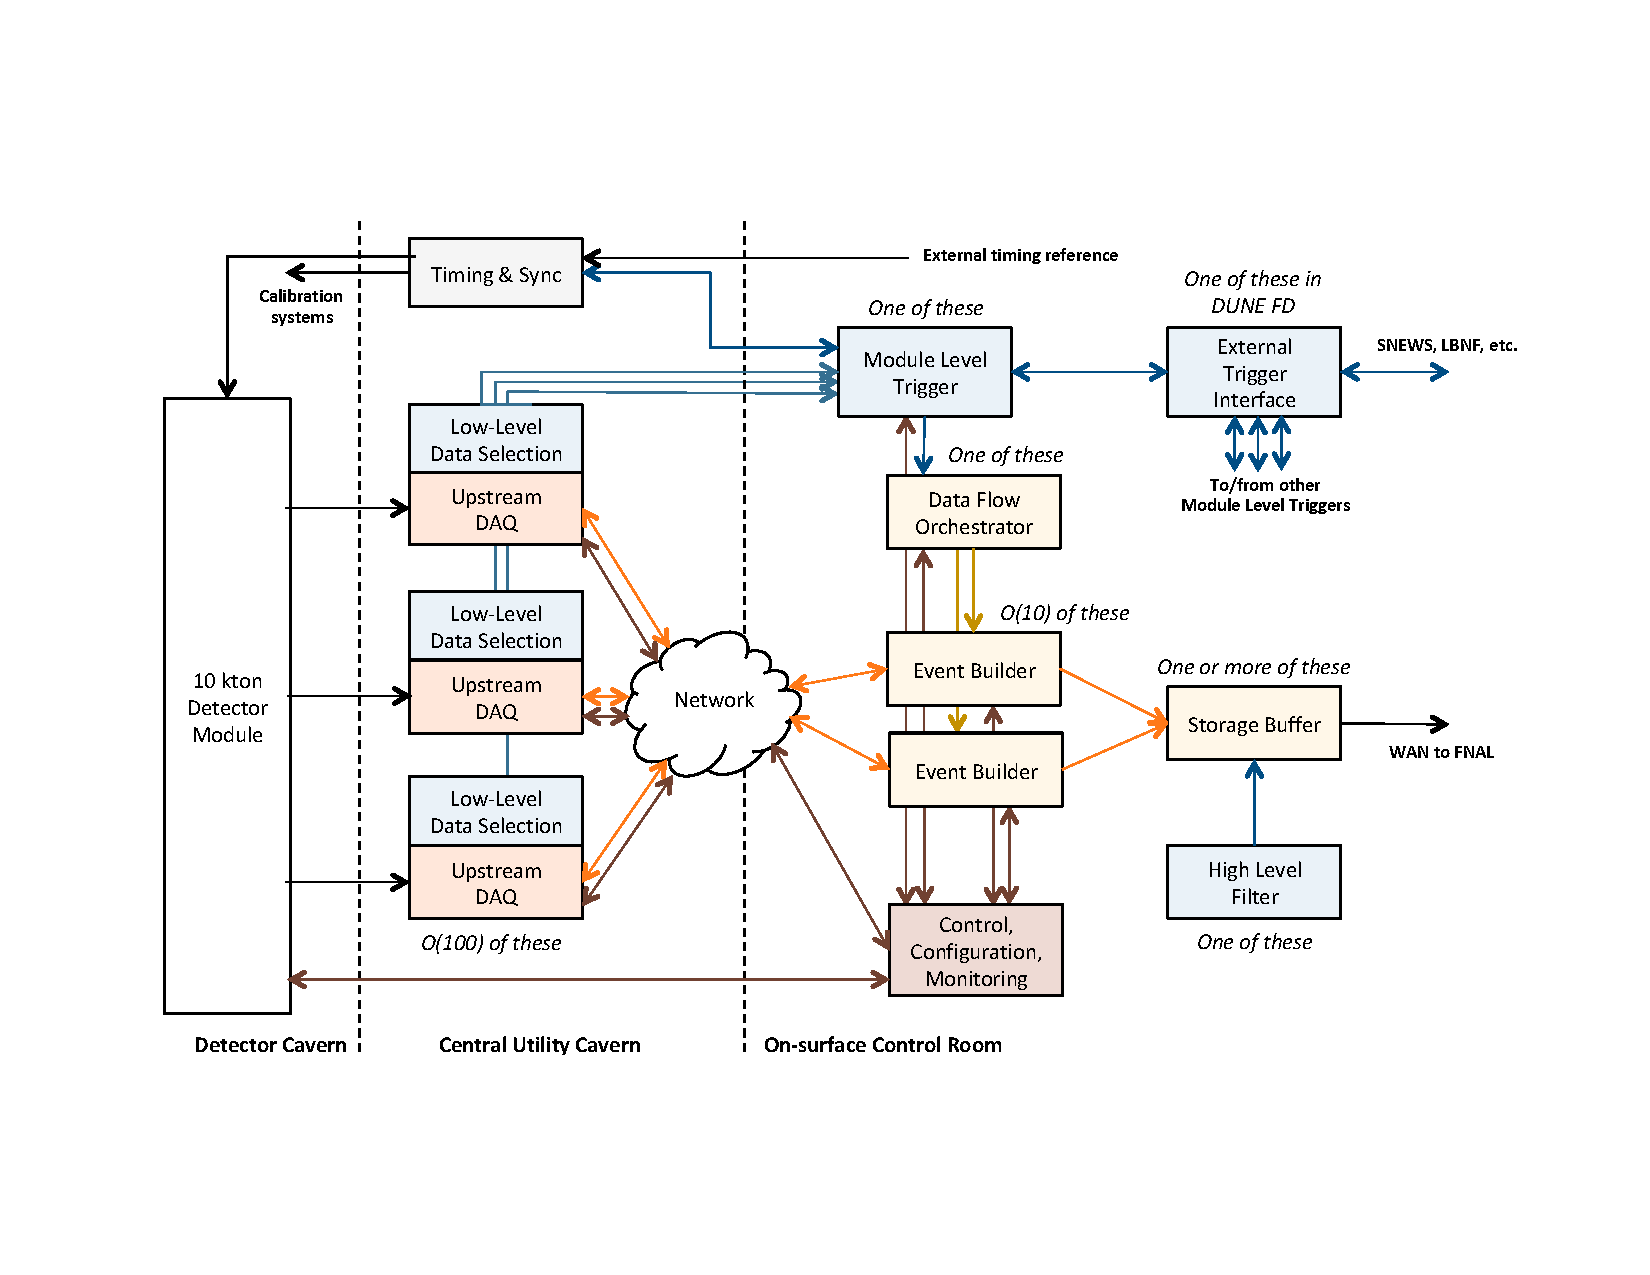
\includegraphics[width=0.8\textwidth,trim=4cm 3cm 4cm 3cm]{daq-layout-2.pdf}
\end{dunefigure}


\subsection{Requirements and Specifications}
\label{sec:daq:requirements}

The \dword{dune} \dword{fd} \dword{daq} system is designed to meet the
\dword{dune} top-level as well as \dword{daq}-level requirements
summarized in 
Table~\ref{tab:specs:DP-DAQ}. 
The \dword{daq}-level requirements ensure that the 
system
can record all necessary information for offline 
analysis of data associated with on- and off-beam physics events, as directed
by the \dword{dune} physics mission, with minimal compromise to
\dword{dune}'s physics sensitivity. The requirements must be met following the 
specifications provided in the same table.
Those specifications are
associated with trigger functionality, readout,
and operations and are described further in the following subsections.

\subsubsection{How DUNE's Physics Mission Drives the DAQ Design}

The \dword{dune} \dword{fd} has three main physics drivers: measuring neutrino \dword{cpv} and related
long baseline oscillation using the high intensity beam provided
by \fnal; measuring off-beam atmospheric neutrinos and searches
for rare processes such baryon-number-violating decays;
and detecting neutrinos from a nearby \dword{snb}. The
\dword{dune} \dword{fd} \dword{daq} system must facilitate data
readout to deliver on these main physics drivers while keeping
within physical (space, power) and resource constraints for
the system. In particular, the off-beam measurements require continuous readout of the detector, 
and the lack of external triggers for such
events requires real-time or online data processing and
self-triggering capabilities. Because the
continuous raw data rate of the far detector module, as received by
the \dword{daq} system, reaches multiple
terabits per second, significant data buffering and processing
resources are needed as part of the design, as specified in
later sections of this chapter.

The \dword{dune} \dword{fd} modules use two active detector components from which the 
\dword{daq} system must acquire data: the \dword{tpc} and the \dword{pds}. 
The two components access the physics by sensing and collecting signals associated with very different sensing time scales.

Ionization charge measurement by the \dword{tpc} for any given activity in the detector 
requires a nominal recording of data over a time window of approximately \SIrange{1}{10}{\milli\second}. 
This time scale is determined by the ionization electron drift speed in \dword{lar} and the detector 
dimension along the drift direction, nominally set to 
\dpreadout.
Early commissioning data will be used to evaluate and optimize this nominal readout time.

On the other hand, the \dword{pds} measures argon scintillation light emission,
which occurs and is detected over a timescale of multiple nanoseconds to
microseconds for any given event and/or subsequent subevent process.

Both the TPC and the PDS data are compressed by the front-end electronics prior
to input to the DAQ.
 
Figure \ref{fig:daq-rates} provides the expected activity rates in a
single far detector module as a function of true energy associated
with given types of signal.
At low energy ($<$\SI{10}{\MeV}), activity is dominated by radiological backgrounds
intrinsic to the detector and
low-energy solar neutrino interactions. Supernova burst neutrinos,
expected to arrive at a galactic \dword{snb} rate of once per century, 
would span the \SIrange{10}{30}{\MeV} range. At higher energies (generally
more than \SI{100}{\MeV}), rates are dominated by cosmic rays, beam neutrino interactions,
and atmospheric neutrino interactions. With the exception of supernova
burst neutrinos, the activity associated with any of these physics
signals is localized in space and particularly in time. Supernova burst
activity, on the other hand, is characteristically distinct, because it can
manifest as up to several thousands of low-energy neutrino interactions
arriving over multiple seconds. Supernova burst neutrinos
are thus associated with activity that extends over the entirety of the
detector and over a relatively long time.

The nature and rates of these signatures necessitate a \dword{daqdsn} strategy that handles two
distinct cases: a localized high-energy activity trigger, prompting an event record readout for
activity associated with a minimum of \SI{100}{\MeV} of deposited energy; and an extended low-energy
activity trigger, prompting an event record readout when multiple localized low-energy activity
candidates with low deposited energy each (approximately \SI{10}{\MeV}) are found over a short (less than
\SI{10}{\second}) time and over the entirety of a \nominalmodsize  module. Because of the high
granularity of the detector readout elements, a hierarchical \dword{daqdss} is used to
provide data processing and triggering and to facilitate optional data reduction and filtering. 

The \dword{daq}  system must have $>$99\% efficiency for particles
depositing $>$\SI{100}{\MeV} of energy in the detector for localized
high-energy triggers. The system's architecture must also provide a 
mechanism for triggering on galactic supernova bursts with $>$95\%
efficiency for a supernova burst producing at least 60 
interactions with a neutrino energy $>$\SI{10}{\MeV} in 12~kt of active
detector mass, during the first \SI{10}{\second} of the burst, per
\dword{dune} requirements. This requirement ensures sensitivity to the
great majority of \dwords{snb} in our galaxy as well as some bursts in small
nearby galaxies, as described in this document's \dword{snb} physics requirements
section. The \dword{daq} architecture must also provide a mechanism for recording
neutrino interactions associated with those bursts over a \SI{30}{\second}
period, with a goal of \SI{100}{\second}. During this period, the full raw
data information must be stored. The rationale for the latter is that most
models of \dwords{snb} show structure in the neutrino flux for up to
\SI{30}{\second}, and there is potential for interesting measurements to be made
up to \SI{100}{\second}.

Offline considerations require the \dword{daq} to reduce the
full \dword{fd} data volume for offline permanent storage to  \offsitepbpy.

Strategies will be developed and validated during commissioning 
and early running that will reduce the data volume through the selection
of data based on the activity in the detector (in time and geographical areas).
As highlighted earlier the DP front-end electronics already performs data compression. 

For planning, the \dword{daq} will allot an average \dword{snb} trigger rate of one per month.
Given current understanding of \dword{snb} rates and the $>$95\%
expected efficiency for a \dword{snb} with at least 60 interactions
each of minimum \SI{10}{\MeV} in true neutrino energy, most such triggers will be due to fluctuations
of low energy radiological backgrounds and, potentially, excess
noise. 
Such triggers will prompt \snbtime of data from the entire module to be read out.
At this average rate and if saved to offline storage, the \dword{snb}
triggers will produce \SI{1.8}{\peta\byte/\year} uncompressed from one
single-phase module. There is, however, no requirement to
permanently store \dword{snb}
data that is deemed, after further offline analysis, to be due to fake triggers.

The capability of recording data losslessly is built into the design
as a conservative measure.
Expected data rates from physics signals of interest that fit the
requirement of \offsitepbpy sent to permanent storage are summarized in Table~\ref{tab:daq:rates} and detailed in~\citedocdb{9240}. Potential bottlenecks are analyzed in~\citedocdb{11461}.

\begin{dunefigure}[Expected physics-related activity
    rates in one FD module]{fig:daq-rates}{Expected physics-related activity
    rates in a single \nominalmodsize module.
}
  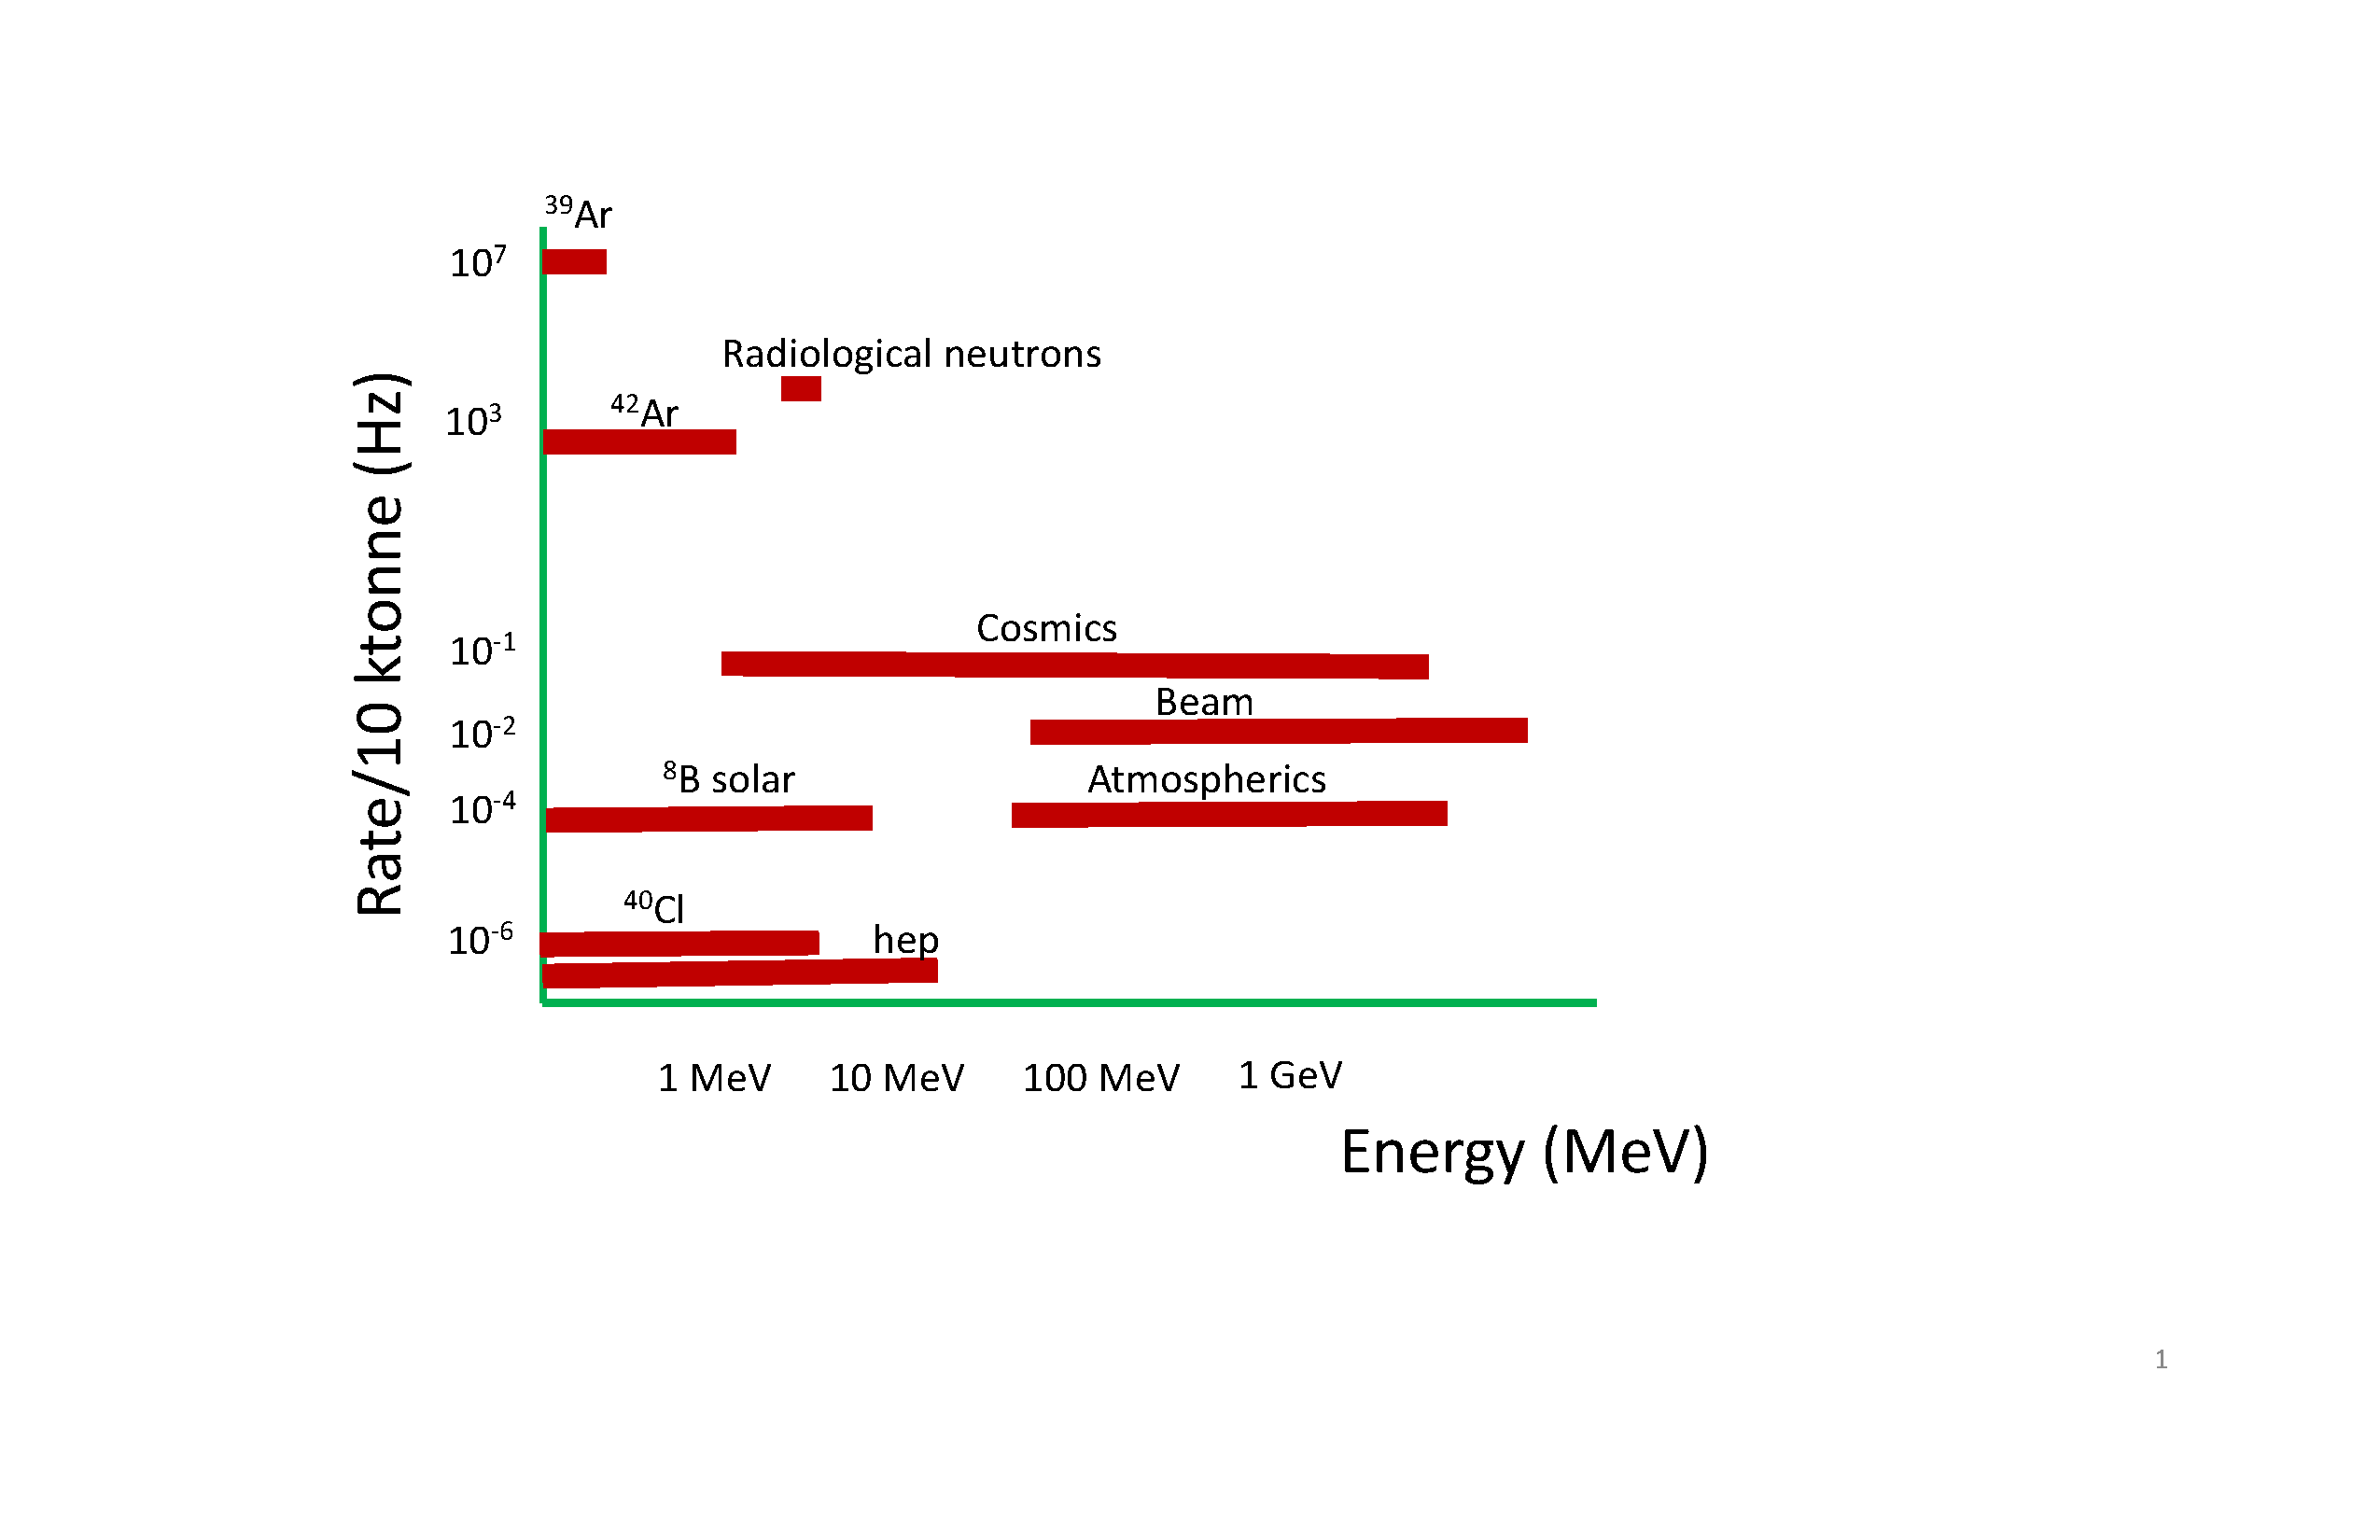
\includegraphics[width=0.7\textwidth,clip,trim=6cm 6cm 10cm 2cm]{daq-event-type-rates-vs-energy.pdf}
\end{dunefigure}

\begin{dunetable} [Expected DAQ Yearly Data Rates] {p{0.25\textwidth}p{0.1\textwidth}p{0.5\textwidth}}{tab:daq:rates}{Summary of expected data rates. The rates assume no compression and are given for a single \SI{10}{\kilo\tonne} \dword{spmod}.
    The equivalent figures for a \SI{10}{\kilo\tonne} \dword{dpmod}   for cosmics and beam data are significantly smaller.
%  \fixme{These numbers are for SP and must be replaced with DP numbers.}
}
Source  & Annual Data Volume & Assumptions \\\toprowrule
Beam interactions & 27 TB & 10 MeV threshold in coincidence with beam
time, including cosmic coincidence; \SI{5.4}{\milli\second} readout \\\colhline
$^{39}$Ar, cosmics and atmospheric neutrinos & 10 PB & \SI{5.4}{\milli\second} readout \\\colhline
Radiological backgrounds & $<2$ PB & $<1$ per month fake rate for SNB
trigger\\\colhline
Cold Electronics calibration & 200 TB & \\\colhline
Radioactive source calibration & 100 TB & $<10$ Hz source rate; single
APA readout; \SI{5.4}{\milli\second} readout \\\colhline
Laser calibration & 200 TB & 10$^6$ total laser pulses; half the
TPC channels illuminated per pulse; lossy
compression (zero-suppression) on all channels\\\colhline
Random triggers & 60 TB & 45 per day\\\colhline
\end{dunetable}

Self-triggering on \dword{snb} activity is a unique challenge for the
\dword{dune} \dword{fd}, and an aspect of the design that has never been demonstrated
in a \dword{lartpc}. The challenge of \dword{snb} triggering is two-fold. 
First, the activity of the individual \dword{snb} neutrino interactions
should be relatively low energy (\SIrange{10}{30}{\mega\electronvolt}),
often indistinguishable from pile up of radiological background activity in the
detector.  Triggering on an ensemble of \bigo{100} events expected on
average in the case of a galactic supernova burst is, therefore,
advantageous; however, this ensemble of events will likely be rare over the
entire detector and over an extended period of \bigo{10}\si{s}, so
sufficient buffering capability must be designed into the system to
capture the corresponding signals. 
Furthermore, to ensure high efficiency in collecting \dword{snb} interactions
that, individually, are below low-energy activity threshold, data from
all channels in the detector will be recorded over an extended and
contiguous period,  which is specified to \SIrange{30}{100}{\second}, around every \dword{snb}
trigger. This time has been defined in consultation with the \dword{dune}
physics groups.

% This file is generated, any edits may be lost.
\begin{footnotesize}
%\begin{longtable}{p{0.14\textwidth}p{0.13\textwidth}p{0.18\textwidth}p{0.22\textwidth}p{0.20\textwidth}}
\begin{longtable}{p{0.12\textwidth}p{0.18\textwidth}p{0.17\textwidth}p{0.25\textwidth}p{0.16\textwidth}}
\caption{Specifications for DP-DAQ \fixmehl{ref \texttt{tab:spec:DP-DAQ}}} \\
  \rowcolor{dunesky}
       Label & Description  & Specification \newline (Goal) & Rationale & Validation \\  \colhline


   
  \newtag{DP-DAQ-1}{ spec:DAQ-readout }  & DAQ readout throughput: The DAQ shall be able to accept the continuous, compressed data stream from the TPC and Photon detectors.  &  \SI{65}{GB/s} per dual phase detector module &  Specification from TPC and PDS electronics &  Modular test on test bench; overall throughput scales linearly with the number of electronics crates.  \\ \colhline
    
   
  \newtag{DP-DAQ-2}{ spec:DAQ-throughput }  & DAQ storage throughput: The DAQ shall be able to store selected data at an average throughput of 2 Gb/s, with temporary peak throughput of 100 Gb/s.  &  \SI{2}{GB/s} average storage throughput; \SI{100}{GB/s} peak temporary storage throughput per dual phase detector module &  Average throughput estimated from physics and calibration requirements; peak throughput allowing for fast storage of SNB data.  &  ProtoDUNE demonstrated steady storage at $\sim$ 40 Gb/s for a storage volume of 700 TB. Laboratory tests will allow to demonstrate the performance reach. \\ \colhline
    


\label{tab:specs:DP-DAQ}
\end{longtable}
\end{footnotesize} 

\subsubsection{Considerations for Design}
\label{sec:daq:considerations}

The \dword{daq} system is designed as a single, scalable system that can
service all \dword{fd} modules. It is also designed so the
system can record and store full detector data with zero dead
time, applying appropriate data reduction through data selection and
compression. The system should be evolutionary, taking advantage of the
staged construction of the \dword{dune} \dword{fd}, thus beginning very
conservatively for the first \dword{dune} \dword{fd} module, but aggressively reducing
the design conservatism with further experience of detector
operations. At the same time, the system is designed to be able to add capacity as required. Most processing and buffering of raw
detector data is done underground, in the upstream \dword{daq} and low
level data selection parts of the
system (see Figure~\ref{fig:daq:layout}), with only event building and data
storage on surface.

Power, cooling, and space are constrained both in the \dword{cuc} and on the surface, limited to \daqpower and \daqracks (out of \cucracks total) in the \dword{cuc}, and \surfdaqpower and \surfdaqracks on the surface for \dword{daq} for all four \dword{fd} modules.
The underground part of the DAQ servicing a DP detector module will require less than half of the active components compared to the DAQ for a SP detector \cite{bib:docdb15544}, and will thus comfortably fit into the space and power allocation foreseen for each detector module.


There are five key challenges for the \dword{dune} \dword{fd} \dword{daq} system: 
\begin{itemize}
\item First, the high overall experiment uptime goal requires \dword{daq} to be stringently designed for reliability, fault tolerance, and redundancy, criteria that aim to reduce overall downtime.

  The \dword{daq} system is fully configurable, controllable, and operable from remote locations, with authentication and authorization implemented to allow exclusive control. The \dword{daq} monitors the quality of the detector data and of its own operational status, as well as automated error detection and recovery capabilities.

\item Second, the system must be able to evolve to accommodate newly commissioned sub-components as they are installed into a detector module that is under construction. 
  The \dword{daq} must also continue to service existing modules that are operational while simultaneously accommodating subsequent detector modules as they are installed and commissioned. 
  To support this ongoing variability, the \dword{daq} will support operating as multiple independent instances or partitions.

  Partitioning will also be supported  within a single detector module for special calibration or debugging runs that are incompatible with physics data taking, while the rest of the detector remains in physics data taking mode. Partitioning, i.e., allowing several instances of the \dword{daq} to operate independently with different configurations on different parts of the detector, will also be important during the installation and commissioning, so experts can work in parallel, e.g., for \dwords{pd} and \dword{tpc}.

\item Third, the \dword{snb} physics requirements require heavy buffering in the upstream \dword{daq}. 

  Implementing a buffer element in the upstream \dword{daq} allows
  the formation and capture of delayed, data-driven data selection
  decisions:
  The trigger accumulates low energy signals over an extended period
  while carrying out the \dword{trigdecision}, thus identifying activity compatible with \dword{snb}.
  The depth of this buffer is determined in
  consultation with physics groups and driven primarily by the need
  to retain all unbiased data while processing up to \SI{10}{s} of
  data for the \dword{trigdecision} preceding a \dword{snb} trigger.
  Collecting data containing information on other types of interactions and decays does not pose additional requirements on the upstream \dword{daq} buffer because the latency required for triggers should be well below \SI{10}{s}.

\item Fourth, the \dword{daq} must support a very wide range of readout windows and trigger rates. This includes acquiring localized events in both time and space up to the very large and rare \dword{snb} detector-wide readouts over \SI{100}{s}.

\item Finally, the \dword{daq} must reduce the volume of data to be permanently stored offline to a maximum of \offsitepbpy.
  The \dword{daq} system should be able to select interesting time windows in which activity was detected, apply lossless compression to data records, and filter records to remove unnecessary data regions.

A programmable trigger priority scheme ensures that the readout for the main physics triggers is never or rarely inhibited, thus making it easy to determine the live-time of these triggers. 


\end{itemize}

Table~\ref{tab:daq:parameters} summarizes the important parameters driving the \dword{daq} design. 
These parameters set the scale of data buffering, processing, and transferring resources that must be built 
into each \dword{fd} module. 

\begin{dunetable}
[Key DAQ Parameters]
{ll}
{tab:daq:parameters}
{Summary of important parameters driving the \dword{daq} design.  
}
Parameter & Value \\ \toprowrule
TPC Channel Count per Module & \num{153600}\\ \colhline
TPC Collection Channel Count per Subdetector (CRP) & 1920\\ \colhline
PDS Channel Count per Module & \num{720}\\ \colhline
TPC \dword{adc} Sampling Rate & \SI{2.5}{\mega\hertz}\\ \colhline
TPC \dword{adc} Dynamic Range& \SI{12}{bits}\\ \colhline
PDS \dword{adc} Sampling Rate & Under study \\ \colhline
PDS \dword{adc} Dynamic Range & Under study \\ \colhline
PDS \dword{adc} Readout Length & Under study \\ \colhline
Localized Event Record Window & \dpreadout \\  \colhline
Extended Event Record Window &  \SI{100}{\second}\\  \colhline
Full size of TPC Localized Event Record per Module (uncompressed) & 4.2 GB \\  \colhline
Full size of TPC Extended Event Record per Module (uncompressed) & 56 TB\\  \colhline
\end{dunetable}


\subsection{Interfaces}
\label{sec:daq:interfaces}

The \dword{daq} system scope begins at the optical fibers streaming raw digital data from the detector active components
(\dword{tpc} and \dword{pds}) and ends at a wide-area network interface that
distributes the data from on site at \dword{surf} to offline centers off
site. The \dword{daq} also provides common computing and network services for
other \dword{dune} systems, although slow control and safety functions
fall outside \dword{daq}'s scope.

Consequently, the \dword{dune} \dword{fd} \dword{daq} system interfaces with the dual-phase TPC electronics, computing, \dword{cisc}, and calibration systems of the %\dword{dune}
\dword{fd}, as well as with facilities and underground installation. The
 interface agreements with the \dword{fd} systems 
are listed in Table~\ref{tab:daq:interfaces} and described
briefly in the following subsections. Interface agreements with
facilities and underground installation are described in Section~\ref{sec:daq:production}.

\begin{dunetable}
[\dword{daq} System Interface Links]
{p{0.3\textwidth}p{0.3\textwidth}p{0.2\textwidth}}
{tab:daq:interfaces}
{Data Acquisition System Interface Links.

% \fixme{Some of these are SP interface   documents and need to be replaced with DP versions.}
}
Interfacing System & Description & Reference \\ \toprowrule
DP Electronics  & Physical, protocol and sw interfaces & \citedocdb{6778}\\ \colhline
PDS Readout & Physical, protocol and sw interfaces &  \citedocdb{6727}{v2} \\ \colhline
Computing & Physical, protocol and sw interfaces &  \citedocdb{7123} \\ \colhline
CISC & Physical, protocol and sw interfaces & \citedocdb{6790}{v1} \\ \colhline
Calibration & Physical, protocol and sw interfaces & \citedocdb{7069} \\ \colhline
Timing and Synchronization & Physical, protocol and sw interfaces &  \citedocdb{11224} \\ \colhline
Integration Facility & Physical interfaces & \citedocdb{7042}{v0} \\ \colhline
Facilities & Physical interfaces &  \citedocdb{6988}{v1} \\ \colhline
\end{dunetable}

\begin{description}
\item[TPC Electronics] The \dword{daq} and TPC Electronics interface is
  described in \citedocdb{6778}.
  The physical interface is in the \dword{cuc}, where optical links from the
  \dword{cro} and \dword{lro} microTCA crates which transfer their compressed data to the
  \dword{daq} \dword{fe} readout (\dword{felix}; see
  Section~\ref{sec:daq:design-upstream}).
  This ensures the \dword{daq} is electrically decoupled from the detector
  cryostat.
  One \SI{10}{Gbps} link per each electronics readout is expected, and has been
  specified as 300m OM4 multi-mode fibers from sfp+ at the
    crate 
%{This is what WIBs use, what about DP crates?}
  to \dword{minipod} on \dword{felix}.

The data format employs for the charge readout lossless compression, achieved with an 
optimized version of the Huffman algorithm.  Compression on average reduces by a factor 10 
the data volume.  The typical occupancy of a 10 Gbit/s data link is then around 2 Gbit/s. 
Each charge readout crate includes ten AMC cards, each digitizing 64 channels. 
Data is compressed on the fly on the AMCs, stored on a local memory buffer and continuously streamed to the DAQ.
Data is transmitted by the AMCs to the DAQ, organized in contiguous time-windows. 
Time-windows are exactly synchronized on the entire detector front-end, thanks to the fact  
that the sampling on all AMC is absolutely aligned with respect to the UTC via the White-Rabbit system.  
At the beginning of each time window the data compression sequence is reinitialized on all AMC channels 
starting from the absolute ADC values and the UTC time-stamp of the first sample of the frame is 
transmitted in a window-header packet to the DAQ. Then each AMC performs, sequentially for its 64 channels,
the transmission of the data packets corresponding to the continuous streaming of the 
time-window. Given compression, the number of bytes used to transmit the time-window may change 
dynamically from channel to channel. An example of possible data format is described in the following,
assuming a time-window lasting \SI{3}{\ms} and containing 4k samples per channel.
The definition of the time-window length is flexible and may be further optimized.
In the given time window the AMC transmits sequentially its data from channel 1 to channel 64 by exploiting multiple data frames.
In order to achieve maximum packing per frame, data from several channels are transmitted in the same frame.
Each data frame starts with a header containing the AMC identifier, the frame number,
the number of channels included in the frame, including the last transmitted channel
which may be truncated and have its data sequence overflowing in the next frame.
Then the frame header provides the list of channel numbers included in the frame and the corresponding number of bytes to be read for each one of them.  For instance in case of a frame containing compressed data from 3 contiguous channels  (n,n+1,n+2) starting from channel number n : n,n+1,n+2,N1,N2,N3.  Where n+2 is the last channel of the frame which may have its data overflowing in the next frame. Immediately after the header the rest of the frame contains the raw compressed data:  N1 bytes for channel n,  N2 bytes for channel n+1, N3 bytes for channel n+2.  The number of channels treated in a frame may vary depending on the compression efficiency. The data format aims at the maximal  occupancy of the data frames, independently of the instantaneous compression fluctuations.

\item[Computing] The \dword{daq} and computing interface is described in \citedocdb{7123}.
 The computing consortium
 is responsible for the online areas of WAN connection between \dword{surf} and
\fnal providing \SI{100}{\Gbps} bandwidth, while the \dword{daq} consortium is responsible for disk buffering
to handle any temporary WAN disconnects and the infrastructure needed
for real-time data quality monitoring.  The computing consortium 
is also
responsible for the offline development and operation of the tools for data
transfers to \fnal. The primary
constraint in defining the \dword{daq} and offline computing interface is the
requirement to produce less than \offsitepbpy 
into final storage at
\fnal. The \dword{daq} and
computing consortia are jointly responsible for data
format definition and data access libraries, as well as real-time data
quality monitoring software. The former is specified in the form of a 
data model documented in \citedocdb{7123}.

\item[CISC] The \dword{daq} and \dword{cisc} interface is described in
\citedocdb{6790}. The \dword{daq} provides a network in the \dword{cuc} for \dword{cisc},  operation information and hardware
monitoring information to \dword{cisc}, and power distribution and
rack status units in \dword{daq} racks. The information from \dword{cisc}
feeds back into the \dword{daq} for run control operations.

\item[Calibration] The \dword{daq} and calibration interface is described in \citedocdb{7069}. 
Two calibration systems are envisioned for the \dword{fd}: a laser calibration system and a neutron generator. 
  Two-way communication between the calibration system and the
  \dword{daq} is needed.  Specifically, the calibration system must
  notify the data selection system, thus informing \dword{trigdecision}
  when activity has been induced in the detector. At the same time, 
the \dword{daq} must provide input to the calibration system, so it can avoid inducing activity in 
the detector during certain periods such as \dword{snb} readout time or during a beam spill.
This second communication will be initiated by the data selection
system and distributed via the \dword{daqeti} and
subsequently through the
\dword{daq} timing system.

\item[Timing and Synchronization] The timing system of the \dword{dune}
  \dword{fd} connects with almost all detector systems and with the calibration
  system and has a uniform interface to each of them. 
  A single interface document, \citedocdb{11224}, describes all these timing
  interfaces. 
  In particular, the DAQ timing system will interface with the White Rabbit
  implementation of IEEE1588-2008 utilized by the \dword{dpmod} electronics by providing the analog signals
1PPS and 10MHz clock derived from the GPS disciplined oscillator.

  Accuracy of timestamps delivered to detector endpoints will be
  $\pm$\SI{500}{\nano\second} with respect to UTC.
Synchronization between any two endpoints in the detector will be less than 
\SI{10}{\nano\second}. Between detector modules, synchronization will be less than \SI{25}{\nano\second}.  
\end{description}

\section{Data Acquisition System Design}
\label{sec:daq:design}

This section begins with an overview of the \dword{daq}
design followed by
descriptions of the subsystem designs and implementation specifics.

\subsection{Overview}
\label{sec:daq:design-overview}

The  \dword{daq} system comprises five distinct subsystems:
%
(1) upstream \dword{daq} (Section~\ref{sec:daq:design-upstream}),
%
(2) \dword{daqdss} (Section~\ref{sec:daq:design-data-selection}),
%
(3) \dword{daqbes} (Section~\ref{sec:daq:design-backend}), 
%
(4) \dword{daqccm} (Section~\ref{sec:daq:design-run-control}), and
%
(5) \dword{daqtss} (Section~\ref{sec:daq:design-timing}).
%
Figure~\ref{fig:daq:layout} shows the physical extent of the subsystems: the
upstream \dword{daq} and \dword{daqtss}  live underground in the \dword{cuc}; \dword{daqdss} occupies
both underground and above-ground spaces; \dword{daqbes} is above-ground
and includes data flow orchestration, event building, and buffering before distribution of data
to offline storage; and \dword{daqccm} extends throughout the entire physical layout of the
system, supported on a private network throughout the \dword{daq} system. Each of these subsystems is described in further
detail in the following subsections. 



Front-end readout is carried out by the upstream \dword{daq} using
custom \dword{fpga} based data receiver board and commodity computing hardware, 
all of which is hosted in 21 servers in the \dword{cuc}. About 40 additional servers execute
subsequent software-based low-level processing of trigger
primitives
generated in the upstream \dword{daq} for the purposes of \dword{daqdsn}. 
The trigger candidates constructed from trigger primitives are propagated to a central server responsible
for further processing and module-level triggering. The module level
trigger also
interfaces to a second server that receives and
propagates cross-module and external trigger and timing
information. The module level trigger considers trigger candidates and
external trigger inputs in issuing a \dword{trigcommand} to the \dword{daqbes}
subsystem. The \dword{daqbes} subsystem 
facilitates event building in a few servers and buffering for built
events on non-volatile storage. Upon receiving a \dword{trigcommand}, the \dword{daqbes}
 queries
data from the upstream \dword{daq} buffers and builds that into an event
record, which is temporarily stored in (a number of) files. Event records are optionally processed in a high-level
filter/data reduction stage, which is part of overall data selection,
 before event records are shipped to \dword{dune} offline. Pervasively,
 the  \dfirst{daqccm} orchestrates data taking 
 (Section~\ref{sec:daq:design-run-control}), and the
 \dfirst{daqtss} provides synchronization and synchronous command distribution
 (Section~\ref{sec:daq:design-timing}). Figure~\ref{fig:daq-conceptual-overview}
 provides a conceptual illustration of the overall \dword{daq} system
 functionality.



\begin{dunefigure}[DAQ system overview]{fig:daq-conceptual-overview}{Conceptual
   Overview of \dword{daq} system functionality for a single \nominalmodsize module}
  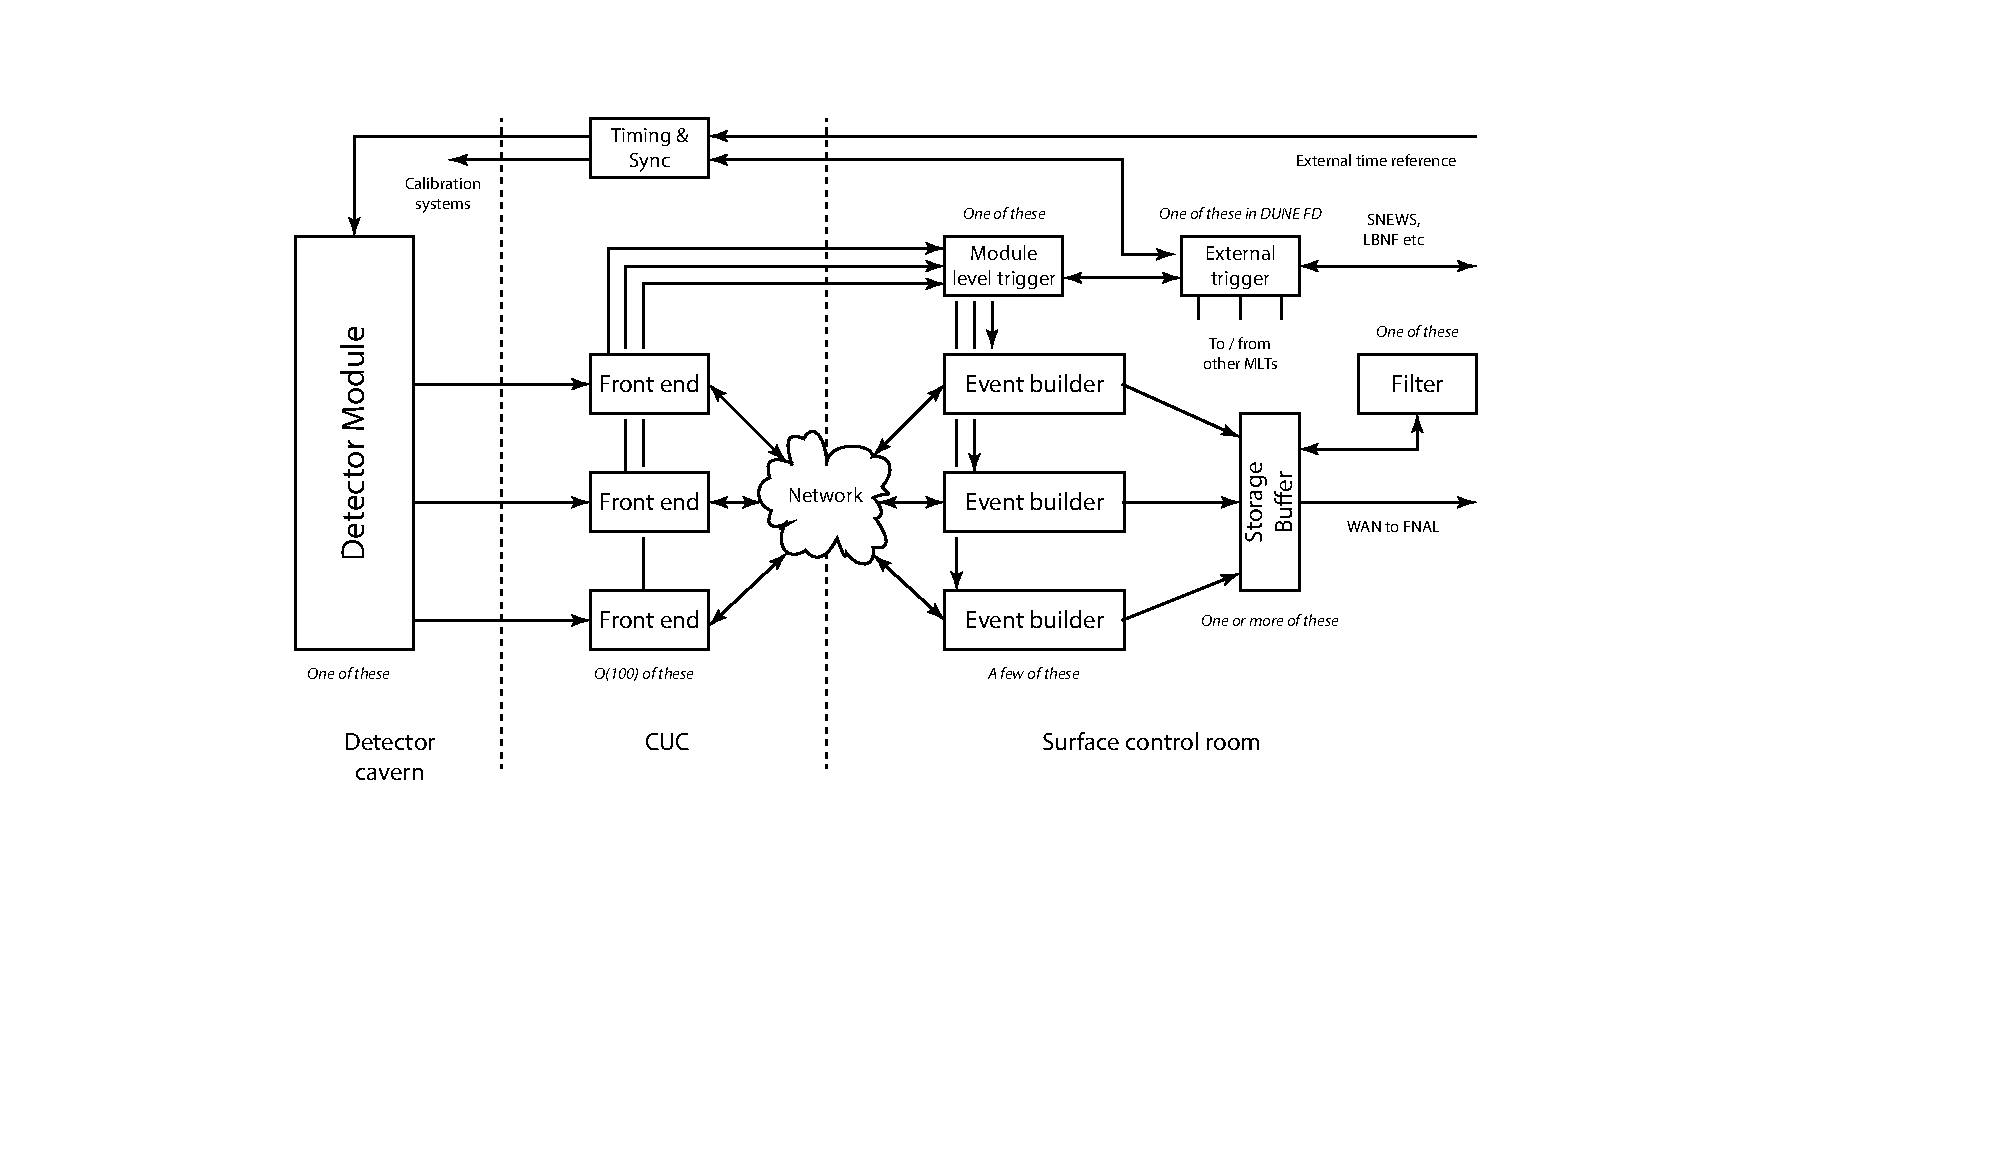
\includegraphics[width=0.9\textwidth]{daq-overview.pdf}
\end{dunefigure}

Key to implementing the \dword{daq} design is the requirement that
the system can be partitioned. Specifically, the system can operate in
as multiple independent \dword{daq} instances, each 
executed across all \dword{daq} subsystems and uniquely mapped among subsystem components. 
More specifically, a given partition may span the entire 
\dword{detmodule} or some subset of it; its extent is configurable at
run start. This ensures continual readout of most of the detector in normal physics data-taking run mode, while
enabling simultaneous calibration or test runs of small portion of the
detector without interrupting normal data taking. 

\subsection{Upstream DAQ}
\label{sec:daq:design-upstream}

The upstream \dword{daq} provides the first link in the data flow chain of
the \dword{daq} system; it receives raw, compressed data from detector electronics.
The upstream \dword{daq} implements a receiver, buffer, and a portion of low-level data
selection (trigger primitive generation; see Section~\ref{sec:daq:design-data-selection}) as detailed in Figure~\ref{fig:daq:readout}.
It is physically connected to the detector electronics via optical
fiber(s) and buffers and serves data to other \dword{daq} subsystems,
namely the \dword{daqdss} and the \dword{daqbes}.

\begin{dunefigure}[DUNE upstream DAQ subsystem and connections]{fig:daq:readout}{\dshort{dune} upstream \dshort{daq} subsystem and its connections.}
  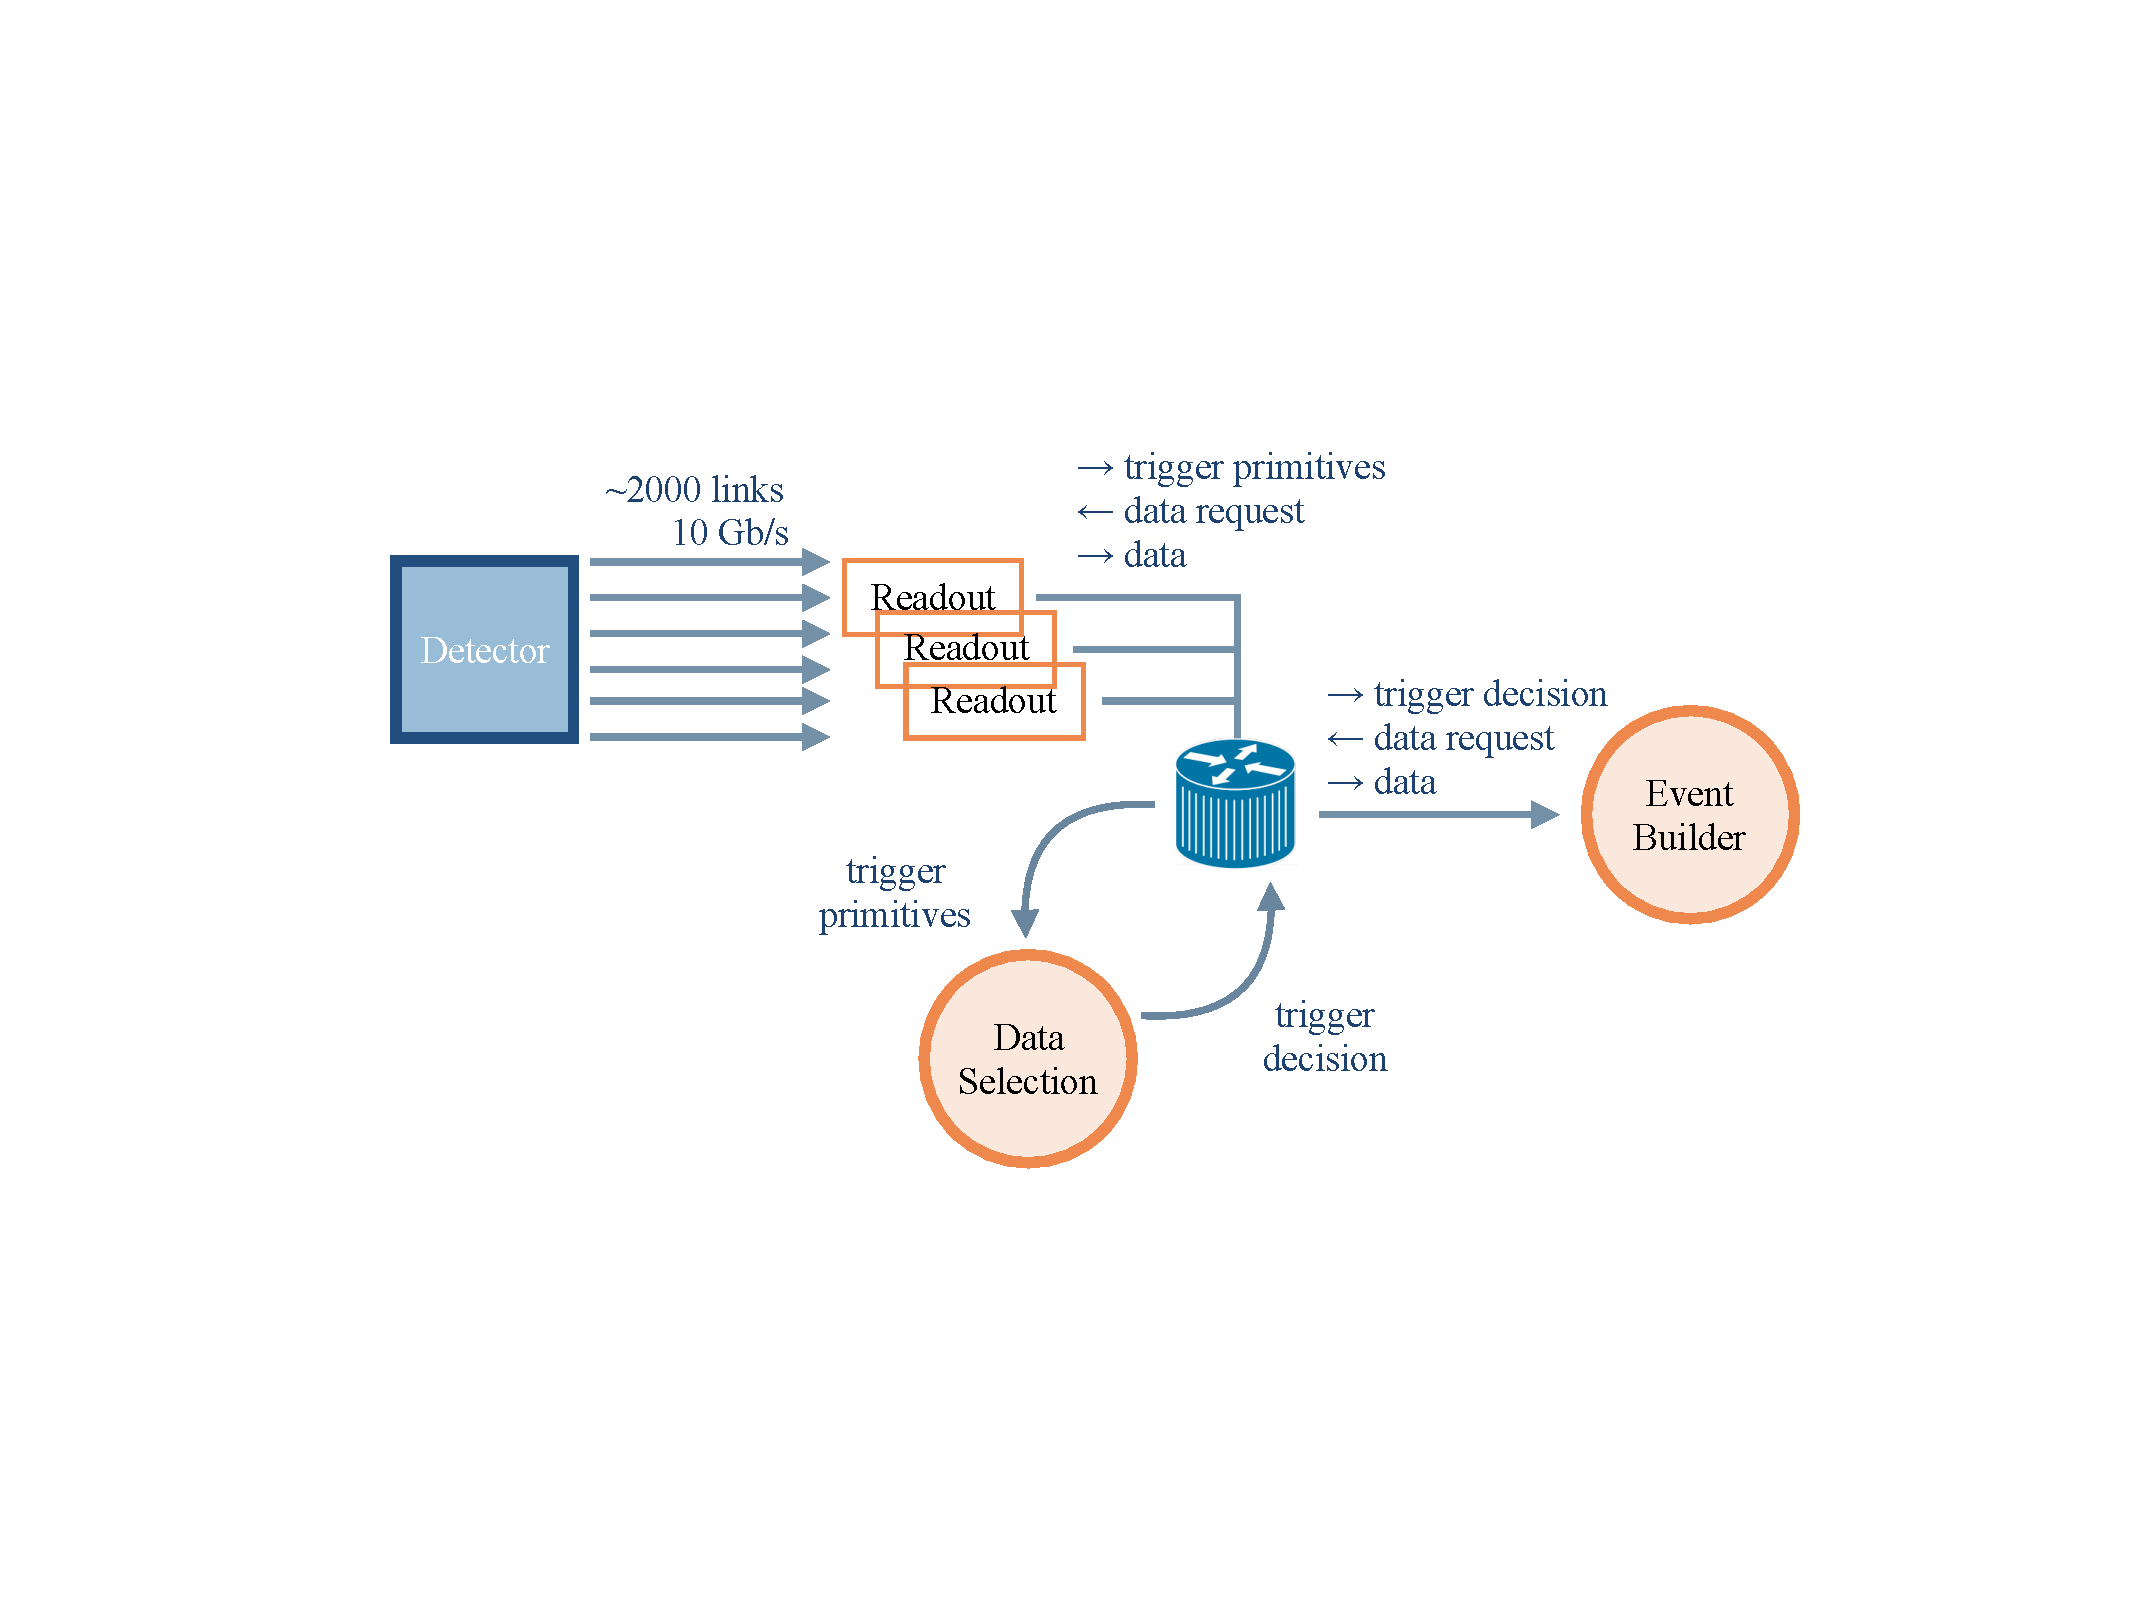
\includegraphics[width=0.8\textwidth]{daq-readout}
\end{dunefigure}

\begin{dunefigure}[Flow diagram of the DUNE upstream DAQ subsystem.]{fig:daq:readout-blocks}{\dword{dune} upstream
    \dword{daq} subsystem functional blocks.}
 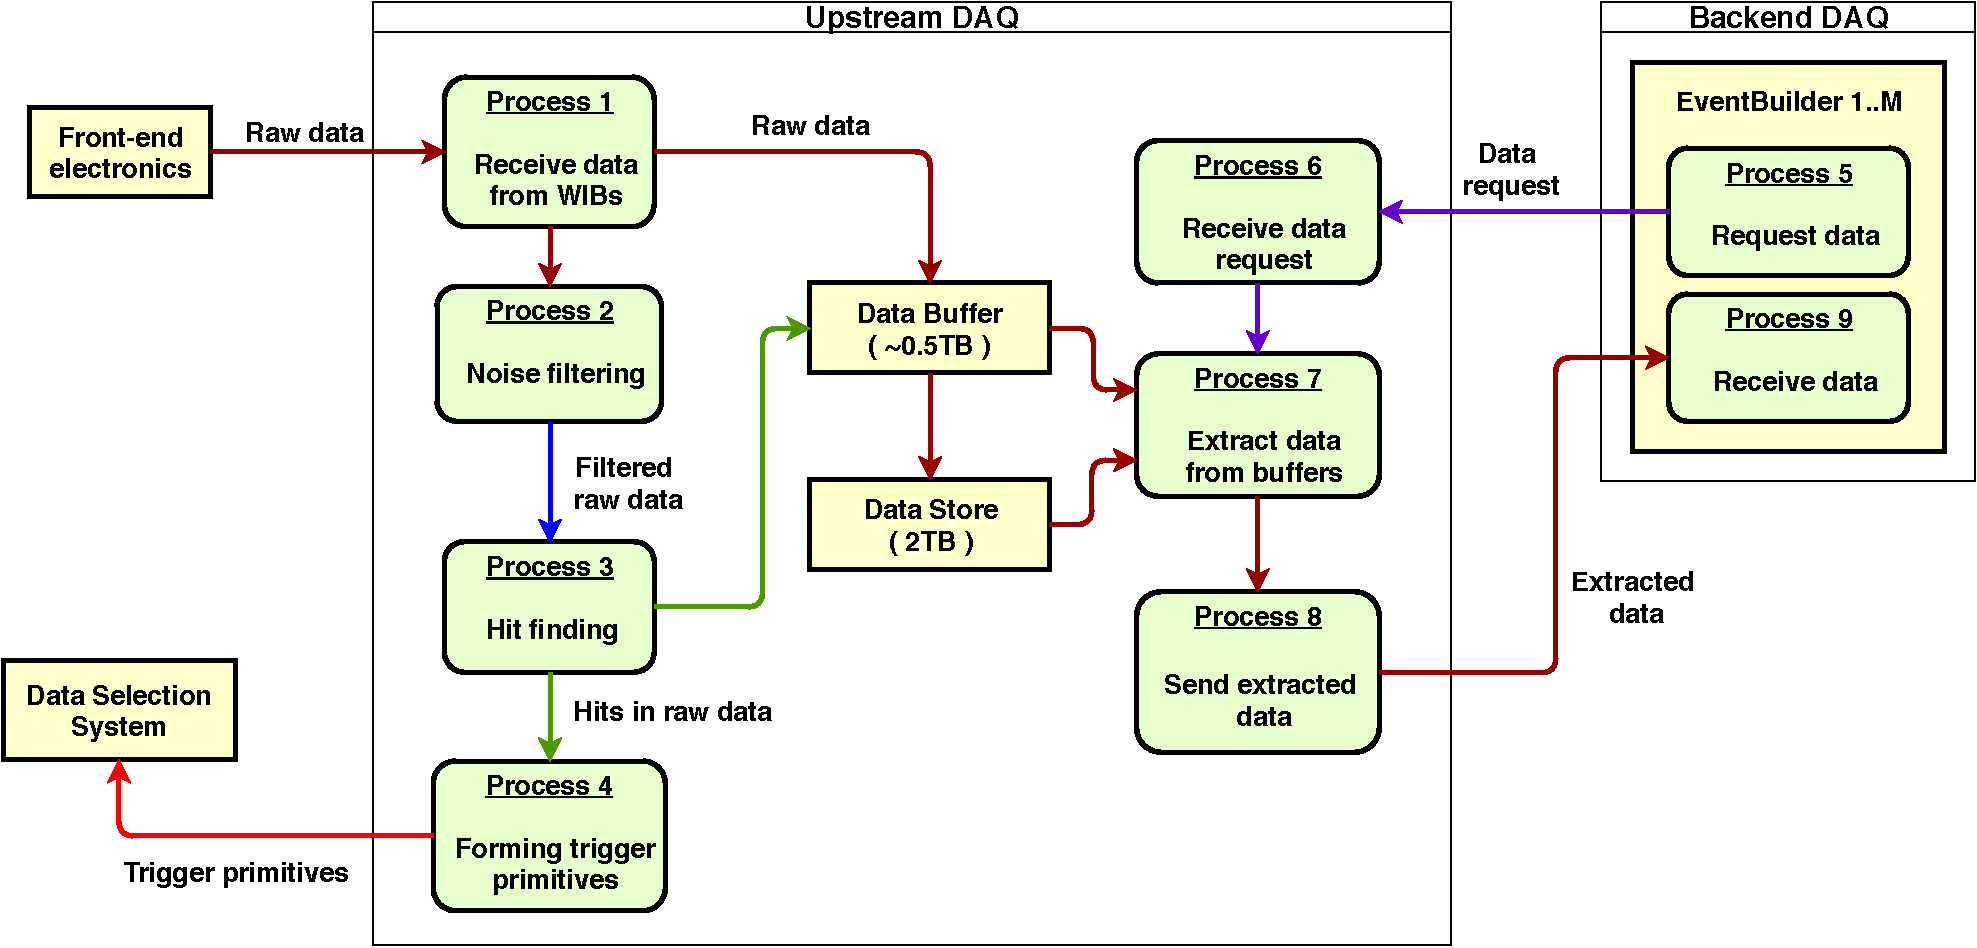
\includegraphics[width=0.8\textwidth]{daq-ud-func-blocks}
\end{dunefigure}

The upstream \dword{daq} system comprises many similar \dwords{daqrou}, each
connected to a subset of electronics from a detector module and
interfacing with the \dword{daq} switched network. In the case of the
\dword{tpc}, 20 functionally identical \dword{daqrou} are each responsible for the readout. In the case of the \dword{pds}, one \dword{daqrou} is responsible for the
readout of raw data from the \dword{pds} subdetectors. 
Each \dword{daqrou} consists of a \dword{fec}, commodity server that hosts a
collection of custom hardware, 
firmware, and software that collectively implement a set of functional blocks.

\begin{enumerate}
\item one dual socket multicore 2U server, with two \SI{10}{\Gbps} and two \SI{1}{\Gbps} ethernet ports for redundant data transmission and control, with at least \SI{128}{\GB} of DDR4 RAM, and \SI{256}{\GB} of persistent storage (e.g. SSD);
\item one \dword{felix} card~\cite{atlas-felix}, each with a PCIe 3.0 x16 interface and supporting ten \SI{9.6}{\Gbps} bidirectional serial optical links;
%\item only for the \dword{tpc} readout, four custom-designed co-processor cards mounted onto the two \dword{felix} cards for additional processing power and data buffering.

\end{enumerate}

The main functional blocks of the upstream \dword{daq} are described below:

\begin{itemize}

  \item The physical interface between the dual-phase detector electronics and the \dword{daq} to
transmit data consists of 10 Gbps point-to-point optical links.
The number of links per dual-phase  \dword{dune} module is 240 for the charge readout system and 5 for the
the light readout system.

To minimize the space and power consumption footprint of the \dword{daq}, 12
links are aggregated into \dword{felix} boards hosted in commercial,
off-the-shelf RU computers.
\dword{felix} is an \dword{fpga}-based PCIe board developed initially for ATLAS
and now proposed or already used in several experiments, including
\dword{protodune}. 
Existing firmware has been adopted and is being adapted to ensure
decoding, format checking of incoming data and online decompression and generation of the trigger primitives
and then to marshal the trigger primitives and compressed data to other blocks of
the upstream DAQ subsystem.

 \item The upstream \dword{daq} subsystem provides access to the
\dword{daqdss} and \dword{daqbes} through a commodity switched network as
illustrated in Figure~\ref{fig:daq:readout}. The network communication
protocol is described in Section~\ref{sec:daq:design-ipc}. The data flow
is handled by the \dwords{daqrou} via software. Dedicated hardware or firmware
development is not required.

\item The data processing functional block is tasked with identifying and forming \dwords{trigprimitive} (see
Section~\ref{sec:daq:design-trigger-primitives}), after a stage of data
reorganization and noise filtering for both the \dword{tpc} and \dword{pds}. \Dwords{trigprimitive} summarize time periods on a channel where the digitized waveform is no longer consistent with noise.
These regions of interest are then used as input to the \dword{daqdss} where they begin the process of forming a \dword{trigdecision}.

In the baseline design, this functional block is implemented in \dword{fpga}.
R\&D studies are ongoing to evaluate alternative implementations (in GPUs or CPUs) that may have advantages in flexibility or cost.

\item In \dword{dune}, the upstream \dword{daq} system is in charge of buffering all
detector data until the \dword{daqdss} has issued a \dword{trigcommand}
(see Section~\ref{sec:daq:design-data-selection}) and until the
\dword{daqbes} (Section~\ref{sec:daq:design-backend}) has requested
and received the corresponding selected data. 
In addition, in the case of a \dword{snb} trigger, data received after
the issuing of the trigger must be buffered for longer to
avoid loss of data due to any possible downstream
bottlenecks. Localized and extended trigger activity are associated
with two rather different time scales and data throughput metrics, and
those collectively dictate the temporary storage technology and scale. 

A \dword{trigdecision} based on localized
activity should require buffering the full data stream for no more than one second.
Extended triggers present a far more challenging set of buffering
requirements; 
early activity from a \dword{snb} may occur at a rate near that of radiological activity.
Theoretical estimates indicate \snbpretime of integration time may be needed for the
\dword{snb} interaction rate to be deemed significantly enough above
background rate to form a trigger decision.
In order to locate interactions in this low-rate period, the full data rate must be buffered until an \dword{snb} trigger may be formed.
The throughput and endurance required by this buffer is satisfied by RAM technology like DDR4.

A second challenge in recording data during an \dword{snb} is to assure
essentially 100\% efficiency for collecting the individual, low-energy
interactions during any given \dword{snb} burst. 
To achieve this, the full-stream of data is recorded for a time duration that should cover the time envelope of the burst.
Guided by \dword{snb} models, this duration is set to \snbtime.
This requires extracting as much as \SI{6}{\tera\byte} (data come into the DAQ already compressed and a factor of ten compression is expected) from the \dword{tpc} upstream \dword{daq} across one 
detector module.
Those data will be temporarily stored in the \dwords{daqrou}. The recorded data will be transferred compatibly with the concurrent traffic on the network to the \dword{daqbes} system in less than a day.

\end{itemize}

Figure~\ref{fig:daq:readout-blocks} shows
the flow diagram of data and control messages within the upstream \dword{daq} 
as well as the main interaction of the upstream \dword{daq} with other subsystems.

\subsection{Data Selection}
\label{sec:daq:design-data-selection}

The \dword{daqdss}  is a hierarchical, online, primarily
software-based system. It is responsible for immediate and continuous processing of a substantial fraction of the entire input data stream. 
This includes data from 
%
\dword{cro} and \dword{lro} subdetectors.
%
From that input, as well as external inputs provided by
the accelerator and detector calibration systems, the \dword{daqdss} must form a \dword{trigdecision},
which in turn produces a \dword{trigcommand}.
This command summarizes the observed activity that led to the decision
and provides addresses (in channel-time space) of the data in the
upstream \dword{daq} buffers that capture raw data
corresponding to the activity.
This command is sent to, then consumed, and executed by the \dfirst{daqbes} as described in Section~\ref{sec:daq:design-backend}. 
It may also be propagated to an \dword{etl} stage, and from there, it may be
distributed to other \dwords{detmodule} or other detector systems
(e.g., calibration) for further consideration.

To facilitate partitioning, the \dword{daqdss}  can be instantiated several times, 
and multiple instances can operate in parallel. Within any
given partition, the \dword{daqdss} will also be
informed and aware of current detector configuration and conditions and
apply certain masks and mapping on subdetectors or their fragments in
its decision making. This information is delivered to the
\dword{daqdss} by the \dword{daqccm} system (Section~\ref{sec:daq:design-run-control}).

Following \dword{dune} \dword{fd} and \dword{daq} requirements, the
\dword{daqdss} must select, with sufficiently high ($>$99\%) efficiency, data associated with calibration
signals, as well as beam interactions,
atmospheric neutrinos, rare baryon-number-violating events, and cosmic
ray events that deposit visible energy in excess of \SI{100}{\MeV}. 
It must also select data associated with potential
\dwords{snb} producing 60 neutrino interactions over a span of \SI{10}{\second} in 12~ktons of active
liquid argon mass each with \SI{10}{\MeV} in neutrino energy, with $>$95\% efficiency. 
Furthermore, to meet the requirement that the \dword{dune} \dword{fd} maintain
$<$\offsitepbpy to permanent storage, the \dword{daqdss}
must make \dword{daqdsn} decisions in a way that allows the \dword{daq} 
system to effectively reduce its input data by almost four orders of magnitude,
without compromising the above efficiencies.

To meet its requirements, the \dword{daqdss} design follows a hierarchical data selection strategy, 
where low-level decisions are fed forward into higher-level ones until a module-level trigger is activated. 
The hierarchy is illustrated in
Figure~\ref{fig:daq:data-selection-hierarchy}. 
At the lowest level, trigger primitives are formed on a per-channel basis, and represent, for the baseline design, a hit on a wire/channel activity summary. 
\Dwords{trigprimitive} are aggregated into \dwords{trigcandidate}, which represent information associated with higher-level constructs derived from trigger primitives, for example ``clusters of hits''. 
\Dword{trigcandidate} information is subsequently used to inform a
module-level \dword{trigdecision}, which generates a \dword{trigcommand};
this takes the form of either a localized high energy trigger or an
extended \dword{snb} trigger, and each prompts the corresponding readout of an
event record. Details on the
exact algorithm implementation for \dword{trigprimitive}, \dword{trigcandidate}, and \dword{trigcommand} generation can be found
in~\citedocdb{11215} and~\citedocdb{14522} and references therein. 
After event-building, further data selection is carried out in the form
of down-selection of event records through a high level
filter. Details on a possible post-event-building filtering algorithm
implementation can be found in~\citedocdb{11311}.

This data selection strategy is applicable to both the \dword{pds} and
the \dword{tpc}, operating in parallel up to the module level trigger stage, where \dword{pds} and \dword{tpc} information can be combined to form a module level \dword{trigdecision}. 
Data selection design efforts have taken the approach of validating
and demonstrating a \dword{tpc}-based data selection. Nevertheless,
the data selection design by construction allows an additional
\dword{pds}-based data selection component to be accommodated within
the same design, which will augment data selection capabilities, efficiency, and robustness.

The \dword{daqdss} subsystem structure is illustrated in
Figure~\ref{fig:daq:data-selection}. The structure
reflects the three stages of \dword{daqdsn}: (1) low level trigger, which consists of
\dword{trigprimitive} generation (facilitated in upstream \dword{daq}; see
Section~\ref{sec:daq:design-upstream}) and subsequent
\dword{trigcandidate} generation; (2) module level trigger; and (3)
high level filter. Each stage is described in further detail in subsequent
sections. An additional subsystem component is the \dword{daqeti},
which serves as a common interface for the
module level trigger of each of the \dword{fd} \dwords{detmodule} and between
the module level trigger and other systems (calibration,
accelerator, and timing system) within a single
\dword{detmodule}. An additional responsibility of the
\dword{daqeti} is to send \dword{snb} triggers
to global coincidence trigger recipients like \dword{snews}
\cite{snews} after sufficient confirmation of trigger quality.

\begin{dunefigure}[Data selection strategy and hierarchy]{fig:daq:data-selection-hierarchy}{Data selection
    strategy and hierarchy.}
 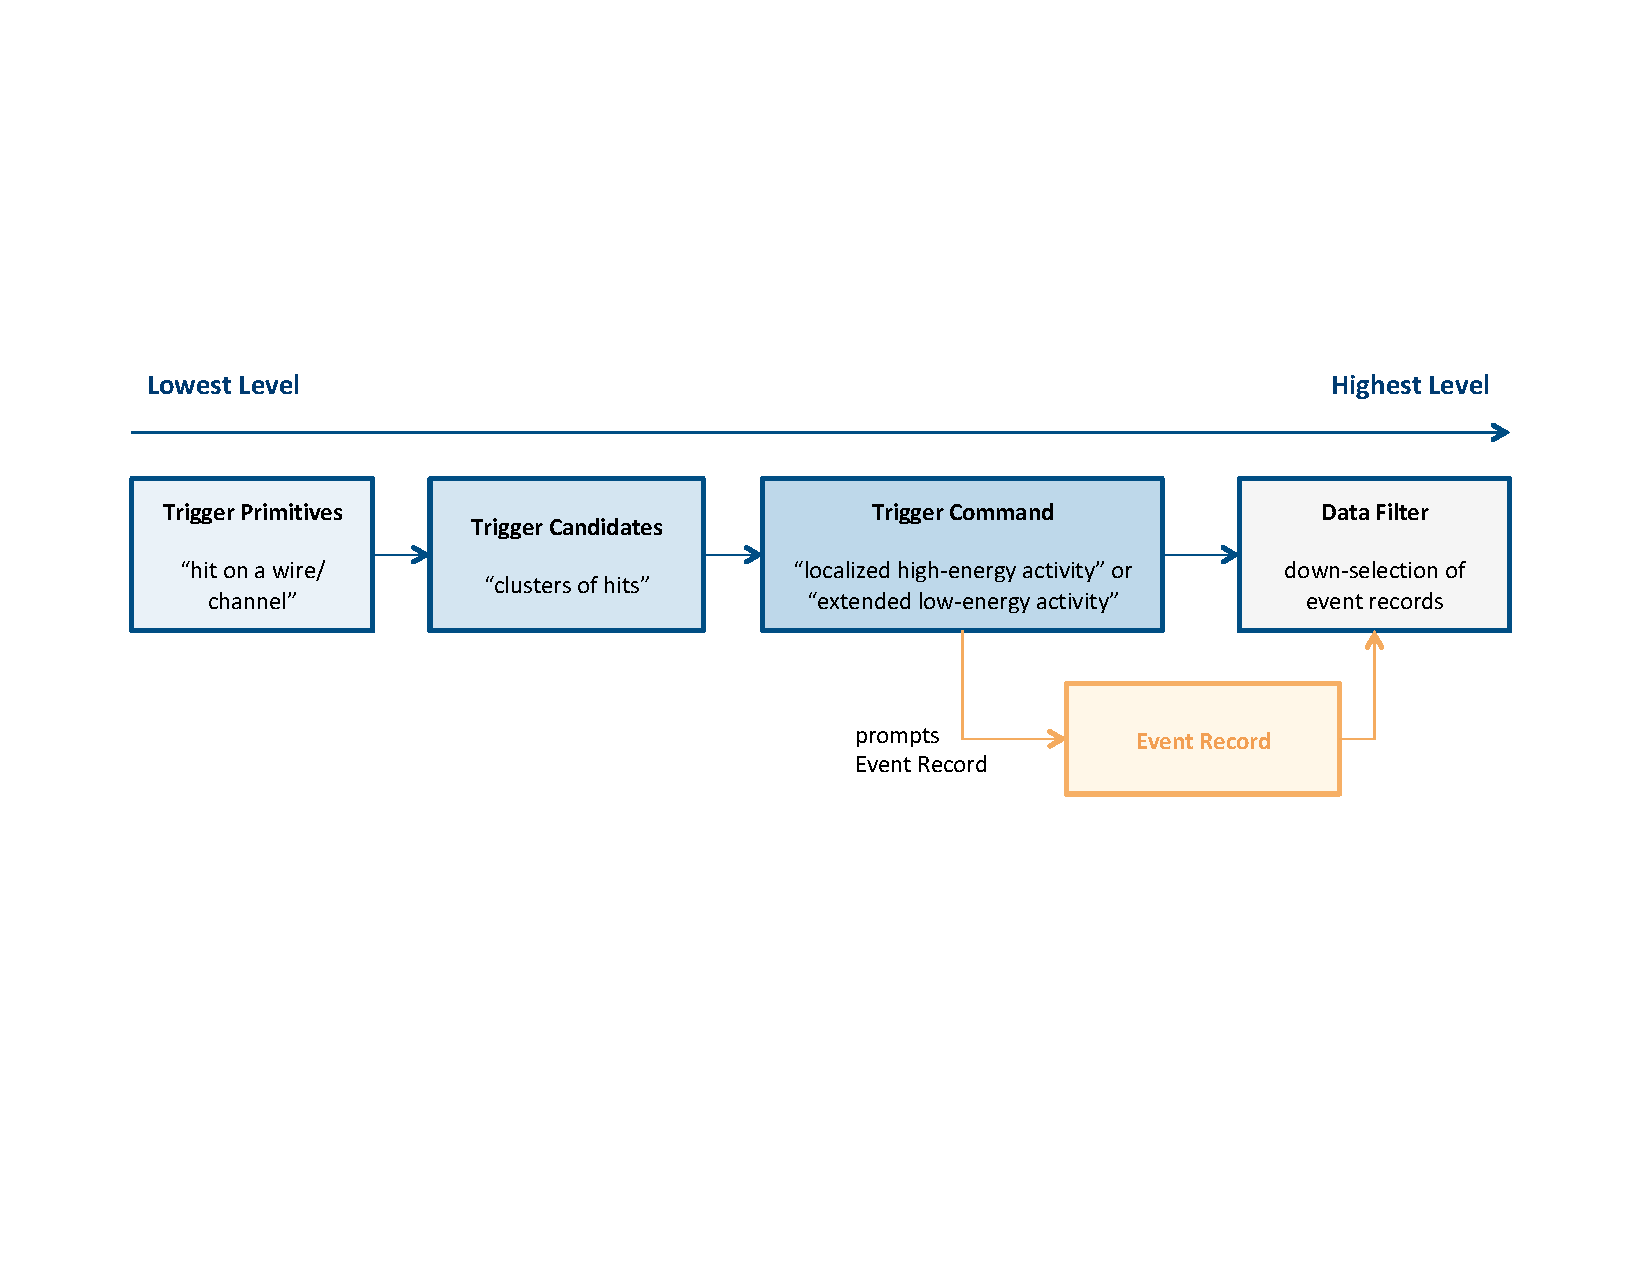
\includegraphics[width=0.9\textwidth, trim=0cm 0cm 0cm 0cm]{DS_hierarchy.pdf}
\end{dunefigure}

\begin{dunefigure}[DUNE DAQ data selection
  subsystem]{fig:daq:data-selection}{Block diagram of the \dword{dune} \dword{daq}
    \dword{daqdss} illustrating hierarchical structure of
    subsystem design, subsystem functionality, and data flow.}
  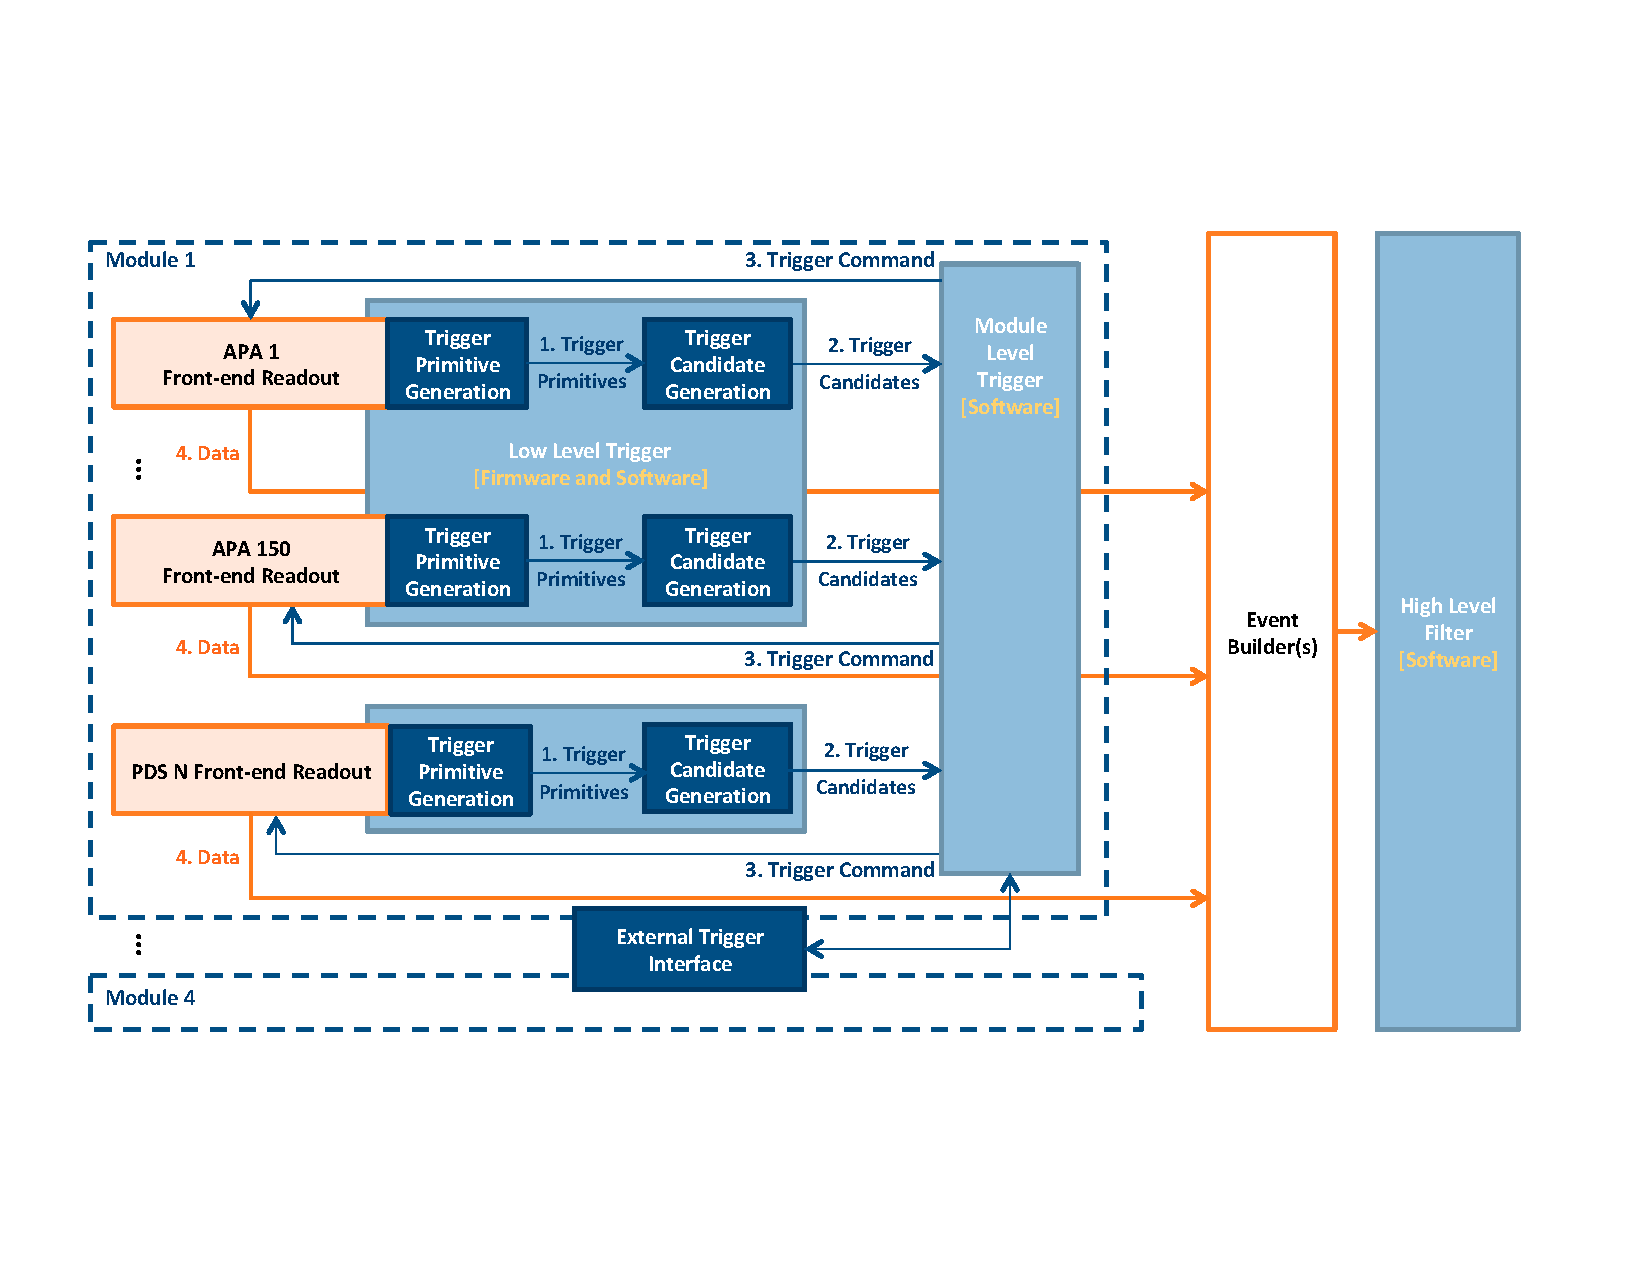
\includegraphics[width=0.95\textwidth, trim=0 2cm 0 0]{DS_summary_2.pdf}
\end{dunefigure}

The first stage of \dword{dune} \dword{fd} operations will trigger on two general
classes of physics, each handled differently at the trigger level:

\begin{description}
\item[High-energy interactions] High-energy interactions include cosmic muons, neutrino beam interactions, atmospheric neutrinos, and nucleon decays. 
  The trigger efficiency for these interactions must be $>$99\% for any given particle type (electron, muon, photon, etc.) that has a localized (confined to a limited number of neighboring channels) visible energy deposition above \SI{100}{\MeV}.
  To achieve this requirement, algorithms for creating high-energy trigger candidates  target a trigger efficiency of 50\% at \SI{10}{\MeV} visible energy, thus ensuring $>$99\% efficiency or higher at \SI{100}{\MeV}.
  This type of trigger is referred to as localized high energy trigger.
  Pushing the high-energy threshold down could enable detection of diffuse supernova neutrinos and solar neutrinos if radiological and neutron backgrounds are low enough.

\item[Low-energy interactions] The primary physics target for
  low-energy interactions is a neutrino burst from a nearby supernova. 
  Low-energy trigger candidates (with thresholds at or below
  \SI{10}{\MeV} visible energy) are generated and are input to an
  extended low-energy trigger data selection algorithm that looks for bursts inconsistent with fluctuations in low-energy background events. 
  The time window for detecting such bursts is tuned to ensure
  nearly 100\% efficiency out to the galactic edge, and the pre-burst
  buffers are sized to handle the associated latency for detection.

\end{description}

\noindent Each trigger type prompts readout
of the entire module but over significantly different time
ranges: localized triggers prompt readout of \dpreadout event records; extended
triggers prompt readout of \SI{100}{\second} event records. 

Ultimately, each \dword{trigdecision} culminates in a command sent to
the \dword{daqbes} subsystem. 
This command contains all logical detector addresses and time ranges
required, so an \dword{eb} can properly query the upstream \dword{daq}
buffers and finally collect and output the corresponding detector data
and the corresponding trigger data. The details for forming this
command are described next, while the operation of the \dword{daqbes} is
described in Section~\ref{sec:daq:design-backend}.

Viable data selection algorithms for the low level and module level triggers already exist, including
algorithms for a module level \dword{snb} trigger.  Monte Carlo simulations have demonstrated that the resulting
\dword{snb} trigger efficiency reaches $>$99\% for any \dwords{snb}
occurring within our galaxy, and efforts to extend this reach to the
Large Magellanic Cloud using refined algorithms are currently under way \cite{bib:docdb11215,bib:docdb14522}. At the same time, the
pipelines of processing required 
for \dword{daqdsn} can be executed using different firmware and software
implementations. Development is actively ongoing to demonstrate
and compare performance of different implementations. In satisfying
the philosophy and strategies of the \dword{daq} design, there is built-in
flexibility in defining whether each element of a pipeline executes on
\dword{fpga}, CPU, GPU, or, in principle, some other future hardware
architecture. A purely software implementation of data selection
(including \dword{trigprimitive} generation) is being
implemented for demonstration at \dword{protodune}; it will be then
modified to match the baseline design in which \dwords{trigprimitive} are
generated in upstream \dword{daq} \dword{fpga}.


\subsubsection{Low Level Trigger: Trigger Primitive Generation}
\label{sec:daq:design-trigger-primitives}

A \dword{trigprimitive} is defined nominally on a per-channel basis. In the case of
the \dword{spmod} \dword{tpc}, it is identified as a
collection-channel signal rising above a (configurable) noise-driven
threshold for a (configurable) minimum period of time (here called a
hit).
A \dword{trigprimitive} takes the form of an information packet that 
summarizes the above-threshold waveform information in terms of its
threshold crossing times and statistical measures of its \dword{adc} samples. 
In addition, these packets carry a flag indicating the occurrence of any
failures or other exceptional behavior during \dword{trigprimitive} processing.


Algorithms for generating \dwords{trigprimitive} are under development
\cite{bib:docdb11275}.  \Dword{trigprimitive} generation proceeds
by establishing a waveform baseline
for a given channel, subtracting this baseline from each sample, maintaining
a measure of the noise level with respect to the baseline, and searching for the waveform to cross a
threshold defined in terms of the noise level.
The  \dword{trigprimitive} or hit is said to span the time period when the waveform is above the noise threshold.
Such algorithms ( e.g.,~\cite{bib:docdb11236}) have been validated
using both Monte Carlo simulations and 
real data from \dword{protodune}. 
\Dword{trigprimitive} generation performance is summarized in
Section~\ref{sec:daq:design-validation}.

The format and schema of \dwords{trigprimitive} are subject to further
optimization because they are further tightly coupled with the generation of
\dwords{trigcandidate}, discussed in the following subsection. Nominally,
each \dword{trigprimitive} comprises the channel address (\SI{32}{\bit}), hit
start time (\SI{64}{\bit}), the time over
threshold (\SI{16}{\bit}), the integral \dword{adc} value (\SI{32}{\bit}),
an error flag (\SI{16}{\bit}), and possibly also
the waveform peak (\SI{12}{\bit}) associated with the hit. 
Thus, \SIrange{20}{22}{\byte} provides a generous data
representation of \dword{trigprimitive} information. 
The \dword{trigprimitive} rate will be dominated by the rate of decay of naturally occurring
$^{39}$Ar, which is about \SI{10}{\mega\hertz} per module. Radioactive
isotopes of krypton may also contribute to the trigger primitive rate,
but based on results from dark matter experiments, this rate is much
smaller than the intrinsic $^{39}$Ar rate. 
This leads to a detector module \dword{trigprimitive} aggregate rate of
\SI{200}{\mega\byte/\second}.
The subsequent stage of the \dword{daqdsn} must continuously absorb and process this
rate providing \dwords{trigcandidate} as described next.

\subsubsection{Low Level Trigger: Trigger Candidate Generation}

At the \dword{trigcandidate} generation stage of the low level trigger,
\dwords{trigprimitive} from individual, contiguous fragments of the
detector 
module are cross-channel and time correlated, and further selection
criteria are applied. This may result in the
output of \dwords{trigcandidate}. 
More specifically, once activity is localized in time and channel
space, we can apply a rough energy-based threshold based on the combined
metrics carried by the cross-correlated \dwords{trigprimitive};
satisfying this criteria defines a \dword{trigcandidate}. 

A \dword{trigcandidate} packet carries information about all the \dwords{trigprimitive}  used in its formation. 
In particular, the packet provides a measure of the total activity represented
by these primitives, as well as a measure of their collective time, channel
location, and extent within the module.
These measures are used downstream by the module level trigger, 
as described more in the next section.

While the selection applied in the previous stage (\dword{trigprimitive}
generation) is driven by a measure of noise, at the \dword{trigcandidate}
generation stage, before applying any thresholds, the rate is driven by
background activity.  
In particular, $^{39}$Ar decays would provide \SI{50}{\kilo\hertz} of
\dwords{trigcandidate} per \dword{apa} face if the threshold was set very low, i.e., at
\SI{0.1}{\MeV}.
Next, activity from the $^{42}$Ar decay chain would be substantial for a
threshold below \SI{3.5}{\MeV}.
Nominally, individual candidates, or groups of candidates nearby in
detector space and time, with measures of energy higher than these two
types of decays, will be passed to the module level trigger. 

This stage of data selection is implemented 40 servers, which receive the \dword{trigprimitive} stream from the upstream \dword{daq} and distribute \dwords{trigcandidate} to the module level trigger
stage, described next, via the \SI{10}{\Gbps} \dword{daq} network. Studies are underway to demonstrate CPU
resource use and latency, as are efforts to demonstrate online \dword{trigcandidate} generation
at \dword{protodune}. \Dword{trigcandidate} generation performance is summarized in
Section~\ref{sec:daq:design-validation}. 


\subsubsection{Module Level Trigger}
\label{sec:daq:mlt}

Data selection is further facilitated as \dwords{trigcandidate} are consumed
by the module level trigger in order to form the ultimate \dword{trigdecision} that prompts the readout of data records from buffers kept by the upstream \dword{daq}. 
The physical (channel and time) location, extent, and energy measure of the
candidates are used at this stage to categorize the activity in terms
of a localized high energy trigger or an extended low energy trigger. 
Specifically, a suitable number of isolated, low energy candidates found in coincidence
over the integration period of up to \SI{10}{\second} across the full \dword{detmodule}
indicate the latter; individual high energy candidates, found
otherwise, indicate the former.

When a particular condition in a category is satisfied, the \dword{trigdecision} is made and a \dword{trigcommand} is formed. 
The \dword{trigcommand} packet includes information about the candidates (and primitives)
that were used to form it. 
The decision also provides direction as to what set of detector subcomponents
should be read out and over what time period (localized or extended as described above). 
The module level trigger publishes a stream of \dwords{trigcommand} and the primary subscriber should be the \dword{daqdfo} of the \dword{daqbes} as described in Section~\ref{sec:daq:design-backend}.

The module level trigger is implemented in \bigo{1} CPU server (with 100\%
redundancy), which
receives the \dword{trigcandidate} stream from the low level trigger stage
of the data selection and distributes \dwords{trigcommand} to the
\dword{daqbes} via the \SI{10}{\Gbps} \dword{daq} network. Studies are
underway to demonstrate CPU resource use and latency, as are
efforts to demonstrate online \dword{trigcommand} generation at \dword{protodune}.
\Dword{trigcommand} generation performance is summarized in
Section~\ref{sec:daq:design-validation}.

\subsubsection{External Trigger Interface}

The \dword{daqeti} provides a loose coupling between the
\dwords{mlt}, sources of external information such as beam spill times
and information to or from components of \dword{dune} \dword{fd}
calibration systems. As an interface between \dwords{mlt}, the \dword{daqeti} receives and distributes information about module-level \dword{snb} \dwords{trigcommand}.
This allows any detector module, which alone may not have satisfied a \dword{snb} trigger requirement, to nonetheless perform an \dword{snb} readout.
The \dword{daqeti} is also responsible for forming a coincidence between module-level \dword{snb} \dwords{trigcommand} and publishing the results, e.g.,~for consumption by the \dword{snews}.

The \dword{daqeti} also receives information about beam spill times from the accelerator.
These times can drive a model of the beam timeline to predict when
beam spills, and consequently beam-related interactions, should occur. 
These predictions can then be sent to the \dwords{mlt}, so they
can either alter \dword{trigdecision} criteria or merely include the
information in contemporaneous \dwords{trigdecision}. The beam time information can also be distributed to components of the calibration system to avoid producing activity in the detector that may interfere with activity from beam neutrinos.

The external trigger interface is implemented in \bigo{1} CPU server (with 100\%
redundancy), with \SI{10}{\Gbps} networking and interfacing hardware
components (to \dword{wr} and \dword{dune} timing system) for timing and external trigger signal I/O.

\subsubsection{High Level Filter}
\label{sec:daq:design-data-reduction}

The last processing stage in the \dword{daqdss} is the
high level filter, which resides in the \dword{daqbes}, and physically,
on the surface at \dword{surf}.
The high level filter acts on triggered, read out, and aggregated data. 
It therefore serves primarily to down-select and thus
limit the total triggered data rate to offline storage, thereby keeping 
efficiency high in collecting information on activities of interest,
while maintaining low selection and content bias, reducing the output data
rate. It may do so using 
further filtering, lossy data reduction, and/or further event
classification.
Because it benefits from operating on relatively low-rate data, it can accommodate a higher level of
sophistication in algorithms for \dword{daqdsn} decisions.

More specifically, the high level filter may further reduce the rate of data output to offline storage by
applying refined selection criteria that may otherwise be impossible
to apply to the pre-trigger data stream.  For example, instrumentally-generated signals (e.g.,~correlated noise)
may produce \dwords{trigcandidate} that cannot be rejected by the module
level trigger and, if left unmitigated, may lead to an undesirably high
output data rate. 
Post processing the triggered data may reduce this unwanted
contamination.
Furthermore, the high level filter can also reduce the triggered data set by further identifying
and localizing interesting activity. A likely candidate hardware
implementation of this level of \dword{daqdsn} is a GPU-based system
residing on surface at \dword{surf}.

To fully understand how much and what type of data reduction may be
beneficial, simulation studies are ongoing \cite{bib:docdb11311},
summarized in Section~\ref{sec:daq:design-validation}, and will
must be
validated with initial data analysis after the
first \dword{dune} \dword{fd} operation. Development efforts are also ongoing to determine the scale of 
processing required by the \dword{fd}.


\subsection{Back-end DAQ}
\label{sec:daq:design-backend}

The  \dword{daqbes} moves data of interest identified by the data-selection system from the readout \dword{daq} buffers, 
serving them to the high level filter and storing the filtered data into the output buffer. From there, 
data will be transferred to permanent storage off-site.

The \dword{daqbes} system accepts \dwords{trigcommand} produced by the \dword{daqdss} as described
in Section~\ref{sec:daq:design-data-selection}.  It queries the upstream \dword{daq} buffers and
accepts returned data as described in Section~\ref{sec:daq:design-upstream}. Finally, it records
\dwords{trigcommand} and the corresponding detector data to the output storage buffer.

The principal components of the \dword{daqbes} are the \dfirst{daqdfo}, \dfirst{eb} and the output
storage buffer (OB) in Figure~\ref{fig:daq:layout}.

\subsubsection{Data Flow Orchestration}

The \dword{eb} stage is implemented as a pool of redundant \dword{eb} processes to maximize the system tolerance to faults and to handle the readout of long SNB events in parallel to nominal readout requests. This asynchronous, parallel readout will be coordinated by a \dword{daqdfo}.  Its operation is illustrated in Figure~\ref{fig:daq:backend} and is discussed here:


\begin{dunefigure}[DUNE DAQ back-end operation]{fig:daq:backend}{Illustration of \dword{dune} \dword{daqbes} operation.}
  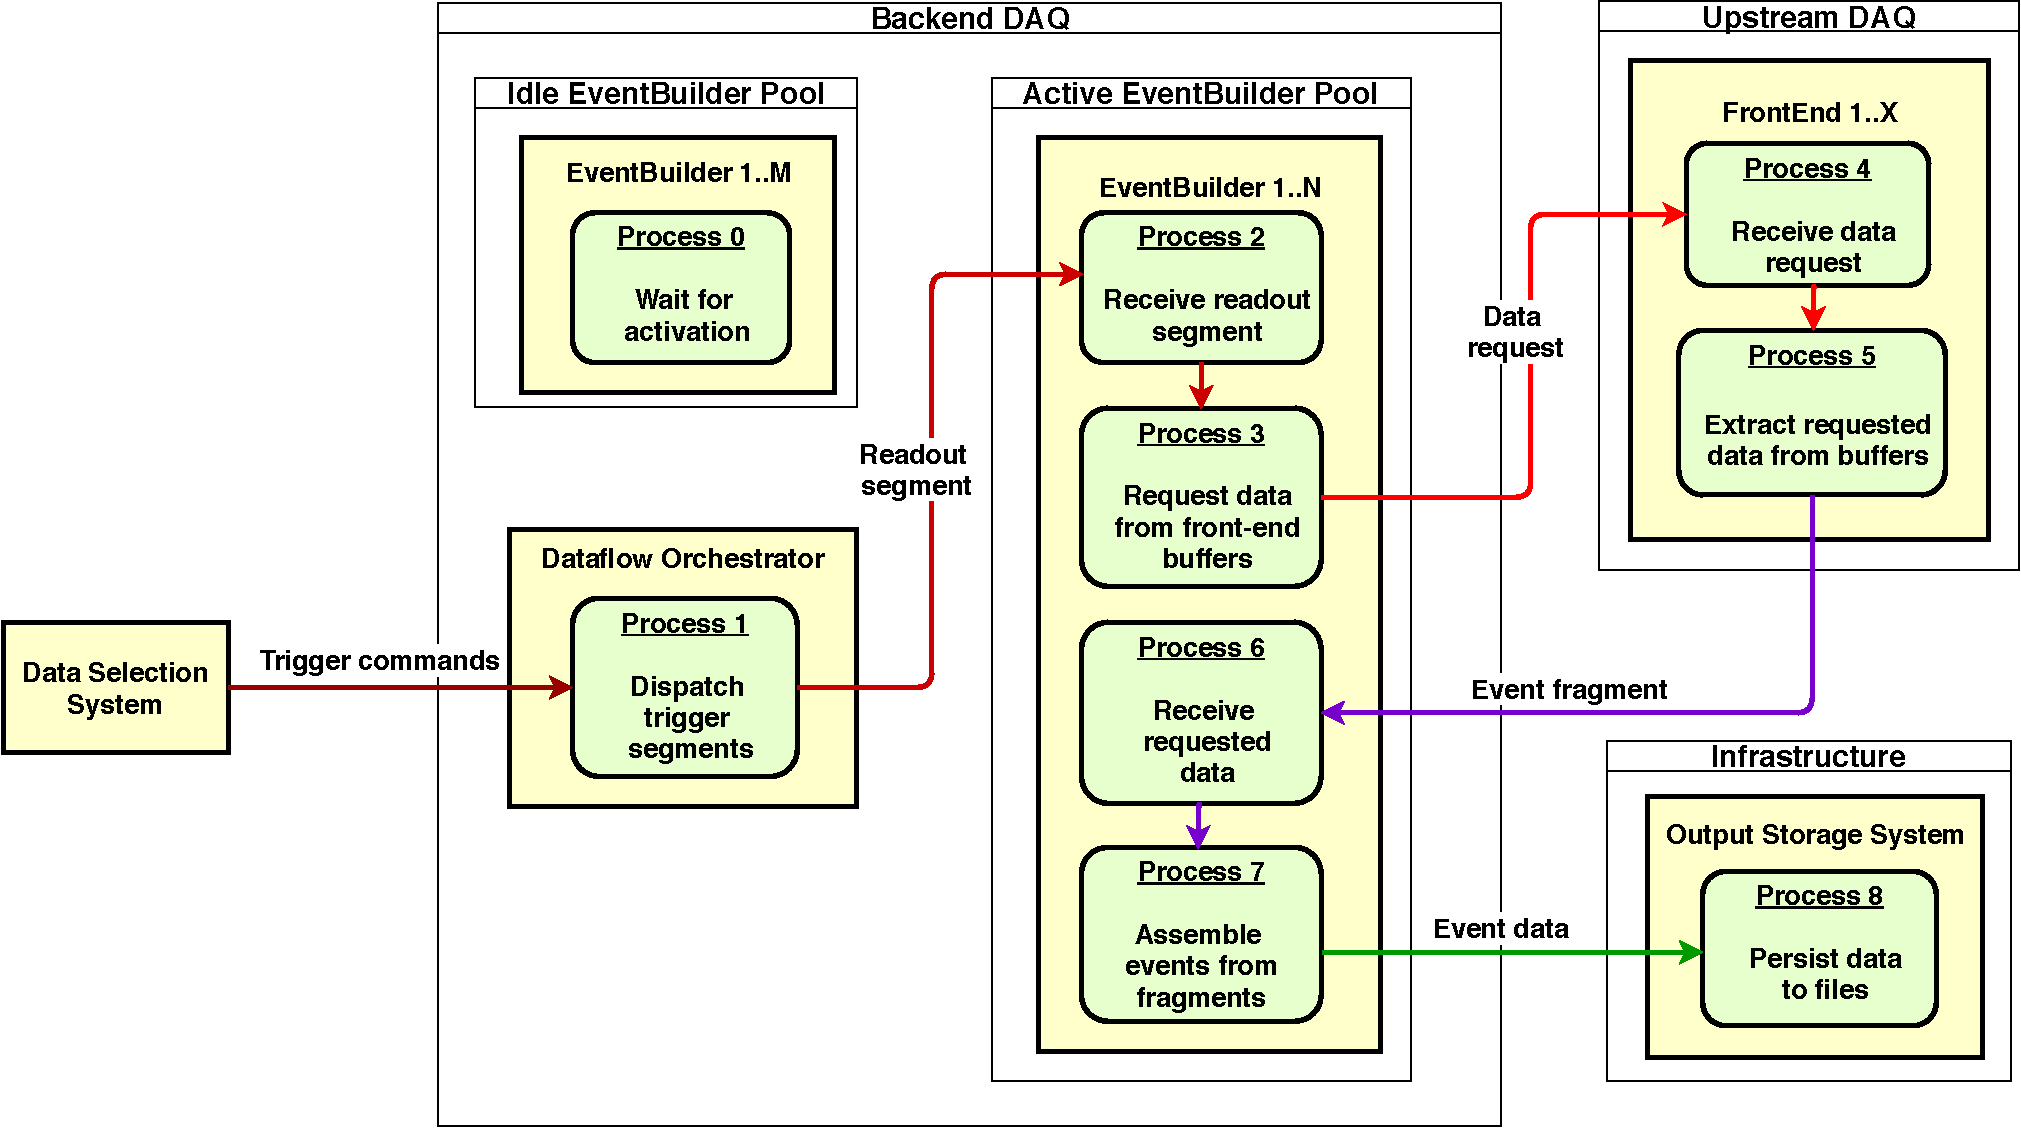
\includegraphics[width=\textwidth]{daq-backend.pdf}
\end{dunefigure}

\begin{itemize}
\item \dword{daqdfo} accepts a stream of \dwords{trigcommand} and dispatches each to an available \dword{eb} process as described in Section~\ref{sec:daq:design-event-builder} for execution.
\item In atypical situations in which there are insufficient event builder resources available to handle the rate of triggers produced by the data selection subsystem, the DFO will alert the DS subsystem that the rate of triggers needs to be reduced.  When such reductions are requested, the \dword{daqdss} will update the calculation of the module-level \dword{daq} livetime appropriately.
\item The DFO will provide relevant data flow status and statistics information to the monitoring processes that are described in Section~\ref{sec:daq:design:ccm:monitoring}. Given its central role and knowledge of the state of available event builder buffers, it will be able to provide important information about the health and performance of the system.
\end{itemize}

\subsubsection{Event Builder}
\label{sec:daq:design-event-builder}

The \dword{daqbes} will provide the instances of the \dfirst{eb} most likely as
\dword{artdaq}~\cite{artdaq} components of the same name. 
As described above, each EB instance will:

\begin{itemize}
  \item Receive a readout segment for execution. Execution entails interpreting the \dword{trigcommand} segment and querying the appropriate upstream \dword{daq} units to request data from the period of time. 
  \item Requests and their replies may be sent synchronously, and replies are expected even if data has already been purged from the upstream \dword{daq} units. (In that case, and empty fragment will be generated with appropriate error flags set).
  \item The received data then processed and aggregated, is finally saved to one or more files on the output storage system before it is transferred offline.
\end{itemize}

As part of this, the EB subsystem will provide book-keeping functionality for the raw data.  This will include the documenting of simple mappings, such as which trigger is stored in which raw data file, as well as more sophisticated quality checks. For example, it will know which time windows and geographic regions of the detector are requested for each trigger, and in the unlikely event that some fraction of the requested detector data can not be stored in the event record, it will document that mismatch.

\subsubsection{Output Buffer}

The output buffer system is composed by the physical hardware resource
to host the incoming data and by the software services handling the
final processing stages through the High Level Filter and the transfer off-site to permanent storage.

It has two primary purposes.  First, it decouples the production of data from filtering and the
transfer of filtered data offline. It provides the elasticity needed by the \dword{daq} to deal with
perturbations in the flow of data, therefore minimizing the impact of temporary loss in filtering
performance due to hardware or software issues. Second, it provides local storage sufficient for
uninterrupted \dword{daq} operation in the unlikely event that the network connection between the
\dword{fd} and \fnal is lost.  A capacity of at least a few \si{\peta\byte} is envisioned,
sufficient to buffer the nominal output of the entire \dword{fd} for about one week even in the case of SNB events. Based on prior experience of the consortium with unusual losses of  connectivity at
other far detector experiment sites, this is a conservative storage capacity value.

The output buffer system will provide the relevant data flow status and statistics information to the monitoring processes that are described in Section~\ref{sec:daq:design:ccm:monitoring}. The knowledge of the health and performance of the of the buffer system will enable the monitoring system to promptly identify and address developing faults before they can have an impact on data taking.


\subsubsection{Data Network}
Upstream \dword{daq}, \dword{daqdss} and \dword{daqbes} \dword{daq} are interconnected by a \SI{10/100}{\Gbps} ethernet network for data exchange.
In particular the upstream \dword{daq} and \dword{daqdss} servers are connected through redundant \SI{10}{\Gbps} links to top-of-rack switches with \SI{10}{\Gbps} uplinks.
The \dword{eb} and Output buffer hardware will support \SI{100}{\Gbps} directly.
The \dword{daq} data network is connected to the \fnal network via a WAN interface.

\subsubsection{Data Model}
\label{sec:daq:design-data-model}

The data model for the DUNE far detector describes the format and characteristics of the triggered data at each stage in the analysis chain, the grouping of the data into logical units such as runs, and the characteristics of ancillary data such as detector configuration parameters and calibration results.

The requirements that these place on the \dword{daq} are primarily in the areas of flexibility and traceability.  The \dword{daq} will have the flexibility to handle the readout of triggers that have a time window that is on the order of a single TPC drift time (for example a trigger associated with a beam gate window), triggers that have a time window of many seconds (such as for a supernova burst trigger), and windows between those two extremes (for detector and electronics studies).  In the area of traceability, the \dword{daq} system will provide the necessary level of detail regarding the conditions that triggered each event, the expected and actual regions of the detector that contributed raw data to each event, the conditions of the detector and electronics during data taking, the version and configuration of the software components used in the \dword{daq} chain, etc.

\subsection{Control, Configuration, and Monitoring}
\label{sec:daq:design-run-control}

The \dfirst{daqccm}, illustrated in Figure~\ref{fig:daq-ccm-subsys}, consist of the software
subsystems to control, configure, and monitor the \dword{daq} system, as well as the detector components
participating to data taking. It provides a central access point for the highly distributed \dword{daq}
components, allowing them to be treated and managed as a single, coherent system, though their
corresponding subsystem interfaces. It is responsible for error handling and recovery, which is
achieved by designing a robust and autonomous fault-tolerant control system. The main goal is to
maximize system up-time, data-taking efficiency and data quality when the system faces programmatic
(i.e. calibrations) and unforeseen (hardware failures or software faults) change of data-taking
conditions. The \dfirst{daqccm} provides an access point, which is delegating user's actions to the
corresponding interfaces. The detector components and infrastructure elements access the \dfirst{daqccm}
subsystems through their provided interfaces. 

\begin{dunefigure}[DAQ CCM subsystem interaction]{fig:daq-ccm-subsys}{Main interaction among the three \dword{daqccm} subsystems.}
 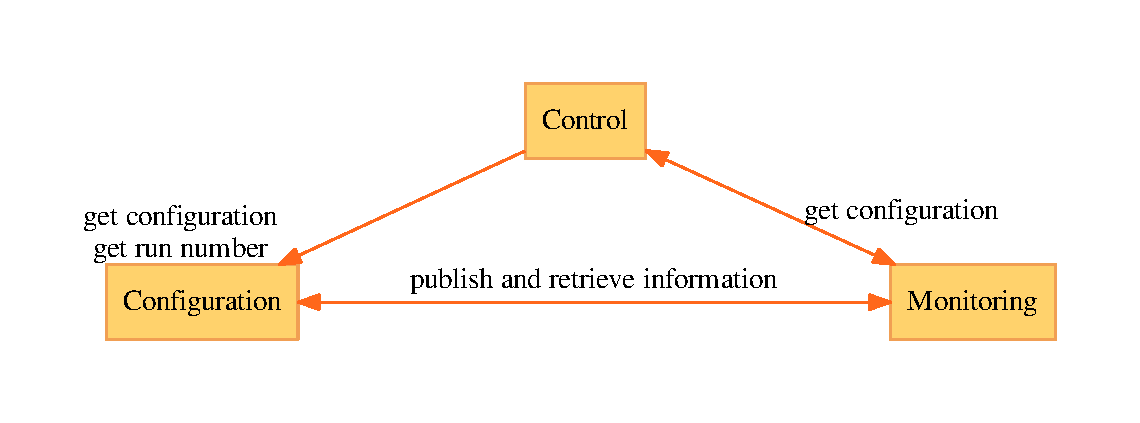
\includegraphics[width=0.9\textwidth]{daq-ccm-subsys.pdf}
\end{dunefigure}

The following sections describe each \dfirst{daqccm} subsystem, covering internal functions and dependencies between each other.

\subsubsection{Access}
\label{sec:daq:design:ccm:access}
Actions are defined as any kind of human interaction with the \dfirst{daqccm}. The access subsystem is responsible for the action delegation to internal function calls and procedures. It's implementation is driven by the control, configuration and monitoring interface specifications, and protects the direct access to detector and infrastructural resources. It also controls authentication and authorization, which locks different functionalities to certain actor groups and subsystems. As an example, only the detector experts can modify front-end configuration through the configuration interfaces, or only an expert user can exclude an APA's readout from data taking. 


\subsubsection{Control}
\label{sec:daq:design:ccm:control}

The control subsystem consists of several components and utilities, and also has additional subsystems to carry out dedicated roles. It enforces the implementation of required interfaces and actively manages \dword{daq} process lifetimes. It operates in a distributed, fault-tolerant manner due to protocols that will drive the FSM for state sharing. 

\begin{dunefigure}[DAQ control subsystem roles and services]{fig:daq-ccm-control}{Roles and services that compose the \dword{daq} control subsystem.}
  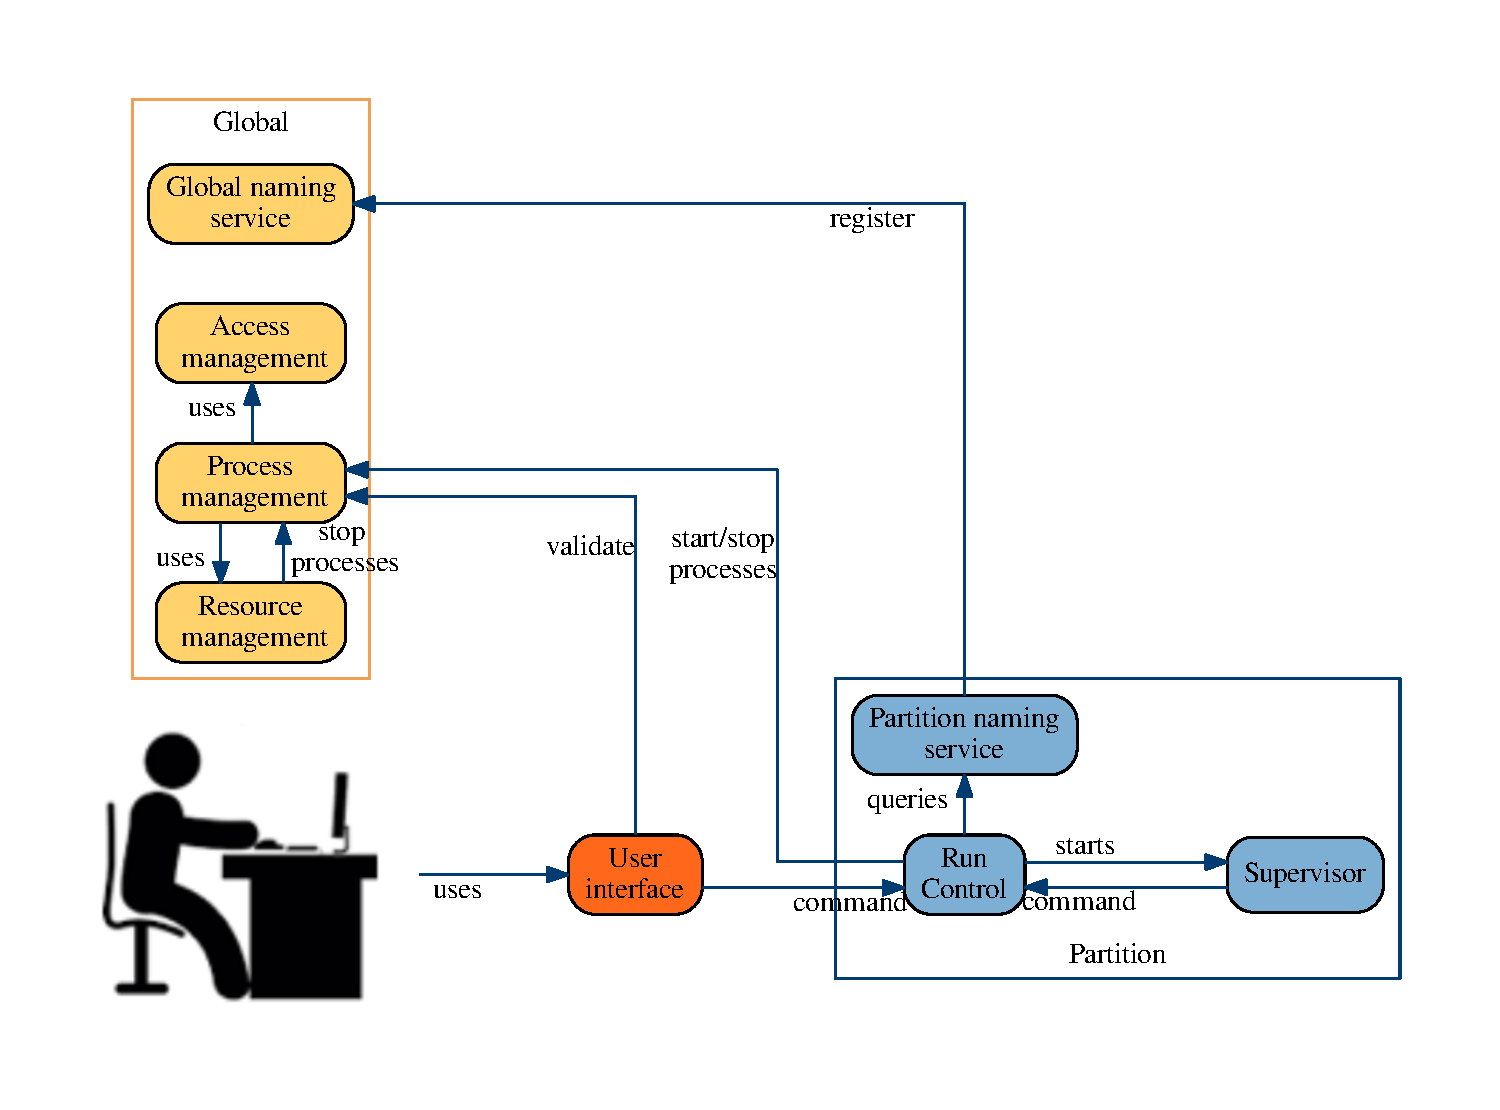
\includegraphics[width=0.8\textwidth]{daq-ccm-control.pdf}
\end{dunefigure}

It contains the following core components:
\begin{itemize}
\item Supervision System - It is responsible for manual and automated control and supervision of \dword{daq} components at any given time. In autonomous mode, the system makes attempts for fault-recovery, failover to backup instances of subsystems, and isolation of problematic regions of the control tree. This is carried out by a hierarchical rule-based planning or fuzzy logic system.
\item \dword{daq} Application - The CCM provides interfaces in order to communicate with processes of the \dword{daq}, and the ability to control and communication with the CCM. The Inter Process Communication (IPC) supports a mechanism to interact with all actors participating to data taking. The Finite State Machine (FSM) enforces the possible states and transitions that are specific to the experiment's components, and also describes them in a uniform way.
\item Run Control - This part of the control subsystem coherently steers the data taking operations. It interacts with all actors participating to data taking in a given partition. It consists of a hierarchical control tree, which can subdivide the \dword{daq} components into separated regions that may be acted upon independently.
\item Resource Management - It provides a global scope of available resources for the \dword{daq} components. This includes the mapping between the detector front-end readout units, processes, servers where they are spawned and required resources for the processes.
\item Process Management - It is responsible for managing process lifetime.
\end{itemize}

\subsubsection{Configuration}
\label{sec:daq:design:ccm:configuration}

The configuration subsystem provides several key elements for the configuration management of \dword{daq} components and detector front-end electronics. It provides a description of system configurations, the ability to define and modify configurations, and graphical user interfaces for the human user to access the data. Data access libraries will hide the technology used for the databases implementation. The subsystem is also responsible for the serialization, persistency, and bookkeeping of configurations. 

\begin{dunefigure}[DAQ CCM subsystem interaction]{fig:daq-ccm-config}{Main components of the \dword{daqccm} configuration subsystem.}
  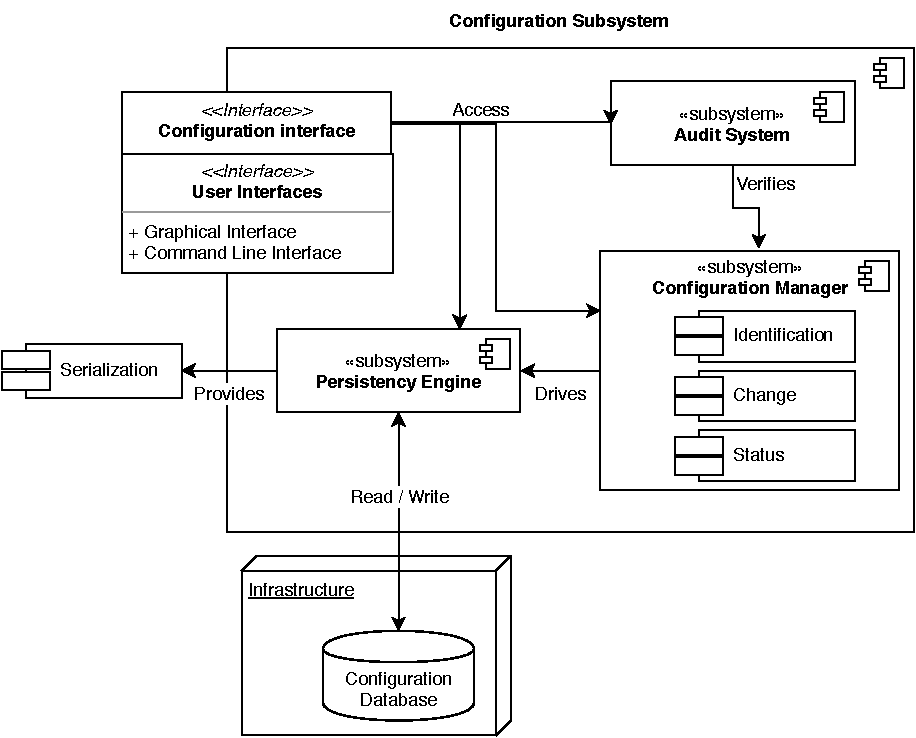
\includegraphics[width=0.8\textwidth]{daq-ccm-config.pdf}
\end{dunefigure}

The main components of the configuration subsystem are the following:
\begin{itemize}
\item Configuration Manager - It consists of the three main components of configuration management systems. The Identification Engine is a set of functionalities that are responsible for the definition of \dword{daq} components and their corresponding configuration specification. The Change Manager is responsible for providing control over altering the configuration specifications of components. The Status Engine is providing status and information about configuration specifications of individual, or set of \dword{daq} elements.
\item Audit System - This important subsystem is supporting the experts and decision making systems to verify the consistency of configuration specifications against the \dword{daq} and detector components. It provides results on mis-configurations and potential problems on configuration alignment and dependencies between components.
\item Persistency Engine - This component provides a single and uniform serialization module, which is strictly followed by every \dword{daq} component. Also responsible for configuration schema evolution and communication with the configuration database. The storage engine privileges will be only read and write operations, not allowing updates and removal of configurations. It also provides a redundant session layer for high-availability and load distribution.
\end{itemize}

The configuration system will mainly consist of standard configuration management components, with a high emphasis on the audit system, in order to verify that the global configuration of the \dword{daqccm} complies with the detector, physics and operational requirements.

\subsubsection{Monitoring}
\label{sec:daq:design:ccm:monitoring}

\begin{dunefigure}[DAQ monitoring subsystem roles and services]{fig:daq-ccm-monitoring}{Roles and services that compose the \dword{daq} monitoring subsystem.}
  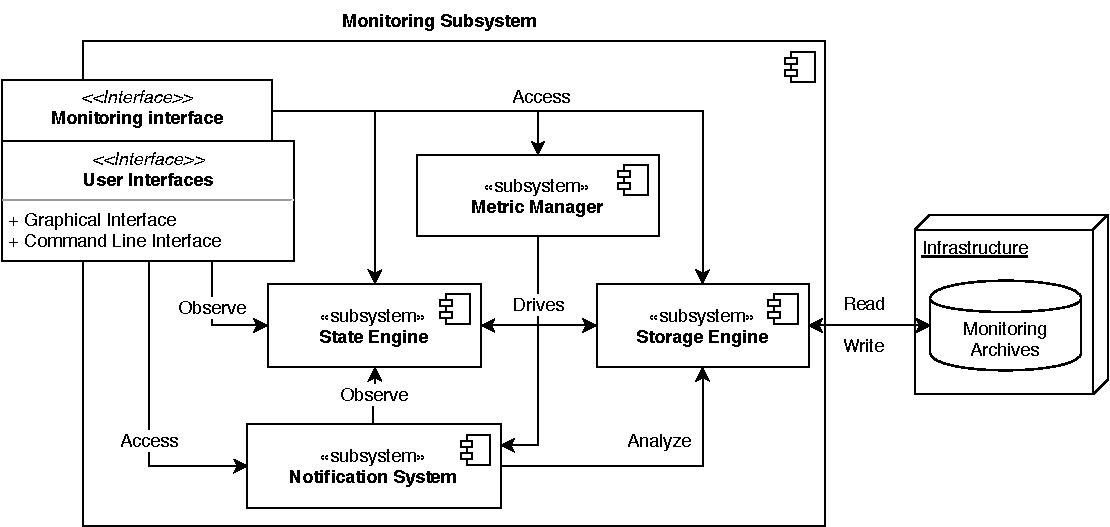
\includegraphics[width=0.8\textwidth]{daq-ccm-monitoring.pdf}
\end{dunefigure}

Highly-scalable and efficient operational monitoring is essential during data-taking periods. Any malfunctioning component of the experiment must be identified and reported as soon as possible. Therefore, the aim of the monitoring subsystem is probing and notifying the status of \dword{daqccm} components, services, and resources. There is also a requirement of \dword{daqccm} infrastructure monitoring and log aggregation. The types of monitoring information vary greatly depending on operational complexity, which require flexibility from the monitoring infrastructure for seamless additions, modifications and aggregated view on service degradation.
It consists of the following main components, also shown in Figure~\ref{fig:daq-ccm-monitoring}:


\begin{itemize}
  \item Metric Manager - It is responsible for the registration of metric data streams and corresponding aggregator functions. This central element is the collection of features and services that provides support for configurable operational monitoring of \dword{daqccm} services. \dword{daqccm} components and services that are registered via the Metric Manager, are reporting monitoring data to the State and the Storage Engines in a publish-subscribe fashion. 
  \item State Engine - This engine is responsible for providing the global state of the system at the current time. It subscribes to a set of registered metrics in the Metric Manager, and records the actual global state of the set for decision making systems (supervision, notification, and visualization).
  \item Storage Engine - Metrics may have different persistency requirements, for which the engine is responsible for archiving the data with the settings of interval, smoothing, etc. It also provides an implementation for the most common communication protocols for the database back ends (SQL, REST, etc.).
  \item Notification System - It is a rule-based system of scheduled and aimed notifications that occur in the case of state combinations. It defines soft and hard states of events and grace periods of alarms.
  \item User Interfaces - Provides graphical and command line user interfaces for monitoring configuration management and visualization of metric data.
\end{itemize}

Monitoring being a key requirement in the industry for computer clusters and their applications, the proposed solution is the adaptation of mature, robust, and open-source third party tools, with the extension of DUNE \dword{daqccm} specific interface implementations and configurations of these monitoring systems. 


\subsubsection{Inter-Process Communication}
\label{sec:daq:design-ipc}

The DUNE FD \dword{daq} is an asynchronous, parallel distributed data processing system. 
It is composed of many independent processes which ingest and produce messages. 
The mechanisms of such message passing are generally called \dword{ipc}. 
Referring to Figure~\ref{fig:daq:layout}, \dword{ipc} is used for both in-band detector data flow between upstream \dword{daq} and back-end \dwords{eb} and for out-of-band messages as part of \dword{daqccm}.  The \dword{ipc} used by the \dword{daqdss} spans both descriptions as it passes derivations of a subset of detector data (trigger primitives, candidates) and culminates in a source of out-of-band message (\dwords{trigcommand}) to direct the readout by \dword{eb} and other components of detector data that is held in the upstream \dword{daq} buffers.

The ZeroMQ~\cite{zeromq} smart socket library is 
the basis of a system being developed and evaluated for parts of both in-band and out-of-band \dword{ipc}. 
As part of the \dword{daqccm}, this includes the issuing of control and reconfiguration commands to and receiving of monitoring messages from essentially all \dword{daq} components. 
As part of \dword{daqdss}, this includes the transfer of \dword{trigprimitive}, candidate and command messages. 
In the upstream \dword{daq} this includes the \dfirst{daqubi} that  provides access to the upstream \dword{daq} primary buffers for queries by \dword{eb} and other components. 
\dword{ipc}  must be implemented broadly across many \dword{daq} systems and ZeroMQ allows their problems to be solved in common, shared software.  As \dword{daqccm} has the most complex \dword{ipc}  needs, this work is organizationally considered part of this system.

As described in~\ref{sec:daq:design-backend}, \dword{artdaq}~\cite{artdaq} utilizes \dword{ipc}  between its back-end components. 
It has been well tested with \dword{protodune} and other experiments. 
\dword{artdaq} may be used for some portions of the \dword{ipc}  described above. 
For example, if the \dword{daqubi} is implemented as an \dword{artdaq} Board Reader it would necessarily use \dword{artdaq} \dword{ipc} . 
This would limit the types of clients that could query for data in the buffers to be \dword{artdaq} modules. 
Understanding how to optimally select an \dword{ipc}  for such parts of the \dword{daq} connection graph is an area of ongoing R\&D effort.

\subsubsection{Hardware}
\label{sec:daq:design:ccm:hardware}

The \dword{daqccm} software suite will run on approximately 15 servers interconnected by a \SI{1}{\Gbps} ethernet network to upstream \dword{daq}, \dword{daqdss}, \dword{daqbes} as well as detector and calibration daq interface elements. While this network has a lower throughput compared to the data network, it has many more endpoints O(2000).

\subsection{Data Quality Monitoring}
\label{sec:daq:design-data-quality}

While the \dword{daqccm} contains an element of monitoring (Section~\ref{sec:daq:design:ccm:monitoring}), here \dfirst{dqm} refers to a subsystem that quickly analyzes the data in order to determine the general quality of the detector and \dword{daq} operation.
This is in order to allow operators to promptly detect and respond to any unexpected changes and assure high exposure times for later physics analyses. 
A \dword{daq} \dfirst{dqm} 
will be developed (including necessary infrastructure, visualization,
and algorithms), which will process a subset of detector data in order
to provide prompt feedback to the detector operators. 
This system will be designed to allow it to evolve as the detector and its data is understood during commissioning and early operation and to cope with any evolution of detector conditions.


\subsection{Timing and Synchronization}
\label{sec:daq:design-timing}

The \dfirst{daqtss} provides synchronous time services to the DAQ and the detector electronics.
All components of the \dword{fd} use clocks derived from a single
\dfirst{gps} disciplined source, and all module components are
synchronized to a common \SI{62.5}{MHz} clock.
%
This rate is chosen in order for this common clock to satisfy the requirements of the detector electronics of both the single-phase and the dual-phase far detector modules.
%
To make full use of the information from the \dword{pds}, the common clock must be aligned within a single detector 
module with an accuracy of \bigo{\SI{10}{\nano\second}}. 
For a common trigger for a \dword{snb} between modules, the timing must have an accuracy of order \SI{1}{\milli\second}.
However, a tighter constraint is the need to calibrate the common clock to universal time derived from \dword{gps} so the \dword{daqdsn} algorithm can be adjusted inside an accelerator spill, which again requires an absolute accuracy of order \SI{1}{\micro\second}. The design of the timing system allows for an order-of-magnitude better synchronization precision than these requirements, allowing a substantial margin of safety and the possibility for future upgrades to front-end electronics.


The \dword{dune} \dword{fd} uses a improved version of the \dword{protodune} timing
system, where a design principle is to transmit synchronization messages over
a serial data stream with the clock embedded in the data. The format
is described in \citedocdb{1651}. The timing system design is
described in detail in \citedocdb{11233}.

Central to the timing system are four types of signals:
\begin{itemize}
\item a \SI{10}{\mega\hertz} reference used to discipline a stable master clock,
\item a \dfirst{pps} from the GPS,
\item a \dword{ptproto} signal providing an absolute time for each \dword{pps}, and
\item an \dfirst{irig} time code signal
  used to set the timing system \SI{64}{\bit} time stamp.
\end{itemize}

The timing system synchronization codes are distributed to the \dword{daq} readout components in the \dfirst{cuc} and the readout components on the cryostat via single mode fibers and passive splitters/combiners.
All custom electronic components of the timing system are contained in two \dword{utca} shelves; at any time, one is active while the other serves as a hot spare.
The \SI{10}{MHz} reference clock and the \dword{pps} signal are received through a single-width \dword{amc} at the center of the \dword{utca} shelf.
This master timing \dword{amc} is a custom board and produces the timing system signals, encoding them onto a serial data stream.
This serial data stream is distributed over a backplane to a number of fanout \dwords{amc}.
The fanout \dword{amc} is an off-the-shelf board with two custom \dwords{fmc}.
Each \dword{fmc} has four \dword{sfp} cages where fibers connect the timing system to each detector component (e.g., \dword{apa}) or where direct attach cables connect to other systems in the \dword{cuc}.

To provide redundancy, two independent GPS systems are used,
one with an antenna at the surface at the Ross shaft, and the other
with an antenna at the surface at the Yates shaft. Signals from either
GPS are fed through single-mode optical fibers to the \dword{cuc}, where
either GPS signal can act as a hot spare while the other is active. 
Differential delays between these two paths are resolved by a second pair of
fibers, one running back from the timing system to each antenna, 
allowing closed-loop delay estimation.
%
The GPS receiver at the  \dword{cuc} generated the 1PPS and 10MHz analog signals which are used to feed
the White Rabbit Grand Master switch of the DP electronics timing system.



\section{Design Validation and Development Plans}
\label{sec:daq:validation}


This section starts with a description of the generic DAQ validation efforts and ends with those specific to interfacing the DAQ with DP
electronics.  As described above, the majority of design elements of the DUNE FD DAQ
are intentionally independent from details of the detector, its electronics and the form and content of the data they provide as input
to the DAQ. 
The differences are accommodated by the thin, custom hardware boundary layer composed of FELIX boards. 
This boundary provides the first and primary translation or ``type
erasure'' so that more generic data forms may then by processed by the DAQ internals.
As it happens, the \dword{pdsp} experiment has been used as a vehicle to validate many solutions to challenges common to servicing both DP and SP
detector technology.

While FELIX absorbs technical differences in formats, rates, etc, some validations described below are sensitive to the information content of
their input data. 
Specifically, the fraction, form and type of the data that is input to
self-triggering studies determines to some extent the performance of the DAQ element being validated.
It can be argued in many cases that a successful validation performed with SP data ensures a successful outcome with equivalent DP data.
The reasons for this become obvious given the following facts which
compare DP \dword{cro} data to SP TPC equivalents:
\begin{itemize}
\item larger signal-to-noise ratio allows thresholds used in
  self-triggering to be more effective.
\item all channels provide unipolar ``collection'' waveforms which may
  be compared immediately and without costly deconvolution to noise
  levels (although, it must be said that both DP and SP cover their
  entire sensitive area with ``collection'' electrodes).
\item the sensitive electrodes are grouped as to provide localized 2D
  segmentation which is at least as effective for self-triggering as
  that which is provided by SP ``collection wires''.
\end{itemize}


Given this practical adaptation of SP data in the validation of DAQ elements for servicing DP detector technology, the following strategy
governs the general validation and development of the \dword{dune}
\dword{fd} \dword{daq} design:
\begin{itemize}
\item Use of \dword{protodune} as a design demonstration and
  development platform. 
\item Use of vertical slice teststands for further development and testing of
  individual \dword{daq} subsystems and for key aspects of the
  overall \dword{daq}
\item Use of horizontal slice tests to demonstrate scaling the design
  where the multiplicity of components in subsystem layers is important.
\item Use of \dword{fd} MonteCarlo simulations and emulations in order
  to augment actual hardware demonstrations at \dword{protodune} and teststands.
\item Benefit from developments and measurements from other ongoing
  LArTPC experiments, including MicroBooNE, SBND, and ICARUS.
\end{itemize}

This strategy reflects the current \dword{daq} project schedule,
provided in Section~\ref{sec:daq:schedule}, which
comprises several phases, including an intense development phase
through 2020 that culminates in an engineering design
review (EDR) in Q1 of 2021. At this milestone, the system design will be
finalized and demonstrated to be capable of meeting the requirements of the
final \dword{daq} system. After the development phase, a
pre-production phase will begin and will end with a production readiness
review (PRR). By then, final designs of all components
will be complete.

The following subsections summarize past, ongoing, and planned development and validation studies and identify how anticipated outcomes will be used to finalize the \dword{daq} design.

\subsection{Design Validation and Development at ProtoDUNEs}


\label{sec:daq:protodune}

The \dword{fd} \dword{daq} consortium constructed and operated a
\dword{daq} system for \dword{protodune} single-phase based on \dword{felix},
develped by ATLAS~\cite{pdsp-felix} which largely represents the general
design for DUNE FD DAQ.
\dword{daq} design and construction for \dword{protodune} began in Q3 of
2016, and the system became operational at the start of the beam data
run in Q4 of 2018.
The detector is continuing to run as of the writing of this document,
recording cosmic ray activity, and providing further input for
\dword{daq} development toward \dword{dune}. 

Besides the differences in horizontal scale between \dword{protodune}
and \dword{dune} FD, their \dwords{daq} exhibit these key differences. 
\begin{itemize}
\item The \dword{protodune} \dword{daq} is externally triggered while
  DUNE FD must be capable of self-triggering. 
\item The \dword{protodune} detectors are on the surface of the Earth
  with minimal overburden. 
  Regardless of trigger mechanism, every readout contains substantially
  more signal activity than expected from an ``average'' readout of DUNE
  FD.
\item The trigger rate of \dword{protodune} detectors is more than two
  orders of magnitude larger than expected at DUNE FD.
\end{itemize}

The first difference illustrates that the production \dword{protodune}
DAQ does not test self-triggering thus validating this ability is of a
prime intereste.
As described in Section~\ref{sec:daq:design-data-selection}, it is the
\dword{daqdsn} which provides self triggering and is a central component
in validation and development plans.
 
On the other hand, the latter two items illustrate that
\dword{protodune} DAQ has in some ways solved harder challenges (at its
given horizontal scale) than will be seen in the DUNE FD. 
The instantaneous rate, per unit of detector is far higher in
\dword{protodune} than DUNE FD. 
The information (signal) content of the data is also higher. 
Thus, local validations on \dword{protodune} assures good performance at
DUNE FD. 
What remains is the relatively ``mechanical'' demonstration that the
required horizontal scaling can be achieved.  

\subsubsection{\dword{pdsp} Outcomes}

Despite being designed for a much more limited horizontal scale than
DUNE, the successful operation of the \dword{protodune} \dword{daq} has
provided several key demonstrations for \dword{dune} FD \dword{daq}, in
particular data flow architecture, run configuration and control, and
back-end functionality.
More specifically, \dword{protodune} has demonstrated

\begin{itemize}
\item Front-end Readout: successful front-end readout hardware and data
  flow functionality for the readout of two out of the six APAs employed
  in protoDUNE.
  This was achieved with two TPC RU's, without co-processor boards, and
  only one APA read out per FELIX board.
  The \dword{dune} DAQ design will ultimately accommodate readout of two
  APAs per FELIX board.
  This readout poses a higher per-fiber data throughput challenge than
  needed for reading out DP crates. 
  However, this tests a synchronous, uncompressed data stream. 
  Testing the receiving of compressed data over UDP from DP crates by
  FELIX will be demonstrated in future validations.

  In addition to data flow functionality, ProtoDUNE Front-end readout
  has been demonstrated to interface to (SP) front-end electronics for
  the purpose of control and configuration. 
  Future validation effort will evaluate what elements need to be
  developed to likewise interface with DP electronics in an equivalent
  manner.

\item Back-end DAQ and Software Infrastructure: successful back-end
  DAQ implementation, including event builder farm and disk buffering.
  This has allowed the development and exercising of system
  partitioning, and provides a basis for scalability to DUNE.
  ProtoDUNE also serves as a platform for further system development

\item Data Selection and Timing: successful operation of the timing
  distribution system, and external trigger distribution to the
  front-end readout.
  Although protoDUNE was externally triggered, the system serves as a
  development platform for data-driven data selection.
\end{itemize}

Besides demonstrating end-to-end data flow, an important outcome of
\dword{protodune} DAQ has been the delineation of interfaces, i.e.~understanding
the exact \dword{daq} scope and the interfaces to TPC, \dword{pds}, and
offline.
The use of commercial off-the-shelf solutions where possible, and
leverage of professional support from CERN IT substantially expedited
the development and success of the project, as did the strong on-site
presence of experts from within the consortium during early installation
and commissioning. 

Outcomes specific to \dword{protodune} subsystems are discussed in
greater detail
in~\cite{Hennessy:CDRReview}. Figure~\ref{fig:daq:protodunedaqpic} shows the
ProtoDUNE DAQ hardware as used during beam data taking.

\begin{dunefigure}[ProtoDUNE DAQ hardware as used during beam data taking]{fig:daq:protodunedaqpic}{ProtoDUNE DAQ hardware as used during beam data taking.}   %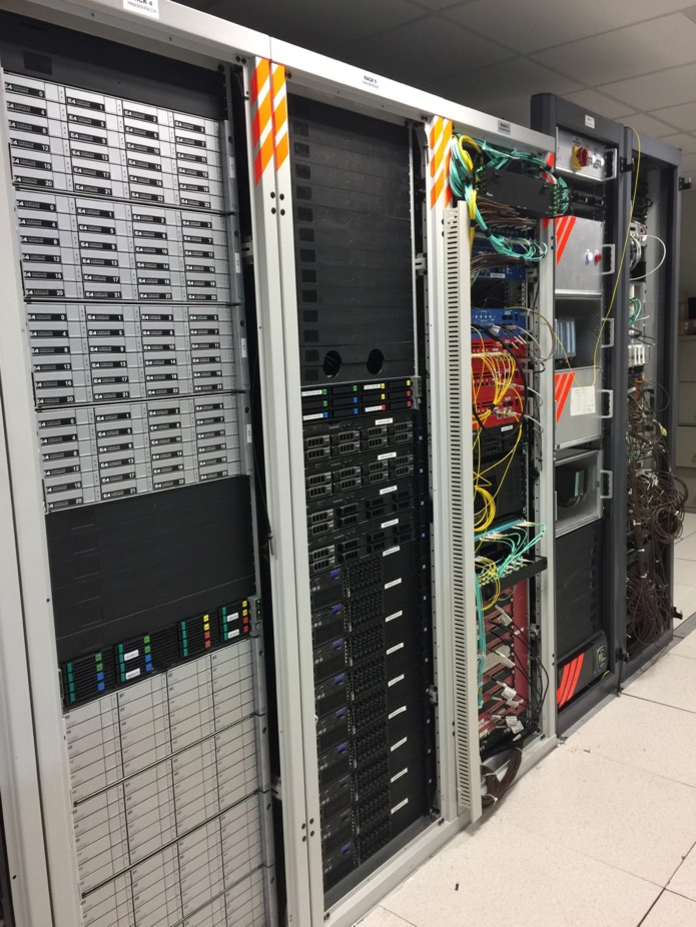
\includegraphics[height=0.5\textheight]{DAQ_hardware_NP04.pdf}
\end{dunefigure}

\subsubsection{\dword{pddp} DAQ architecture}

The \dword{pddp} \dword{daq} system is a Ethernet network based \dword{daq} system which can acquire data at high bandwidth (up to 20 GB/s).
It includes exactly the same Front-End  (FE) elements design as the system foreseen for the 10 kton dual-phase module and similar back-end (BE) architecture.  

The front-end digitization units (AMCs) are contained in uTCA crates. Each charge readout crate, located in front of the corresponding signal feedthrough chimney on the cryostat roof can include up to 10 AMC reading each 64 channels for a total of 640 channels per crate digitized at 2.5 MHz. A uTCA crate is a 10 Gbit/s network system connecting the AMC with its own switch included in the crate controller (MCH). The MCH of each crate is connected with a dedicated 10 Gbit/s to a Level 1 (L1) event builder.  The back-end  \dword{daq} system of \dword{pddp}  consists of two levels of event builder machines Level 1 and Level 2 (L2)  plus the network infrastructure and the online storage/processing facility.  The L1 event builders are connected via several links at 40 Gbit/s to the Level 2 (L2) event builders and to a high bandwidth distributed storage system (EOS), the network infrastructure ensures total 20 GB/s bandwidth.  
The task of the event builders is to receive in input the data flow from the front-end system, to build the events and cluster them in data files. Eventually these data files are written on the distributed EOS file system of the local storage servers.

A global sketch of  the network architecture of \dword{pddp} is shown in picture \ref{fig:BE_network}

\begin{figure} [h!]
 \centering
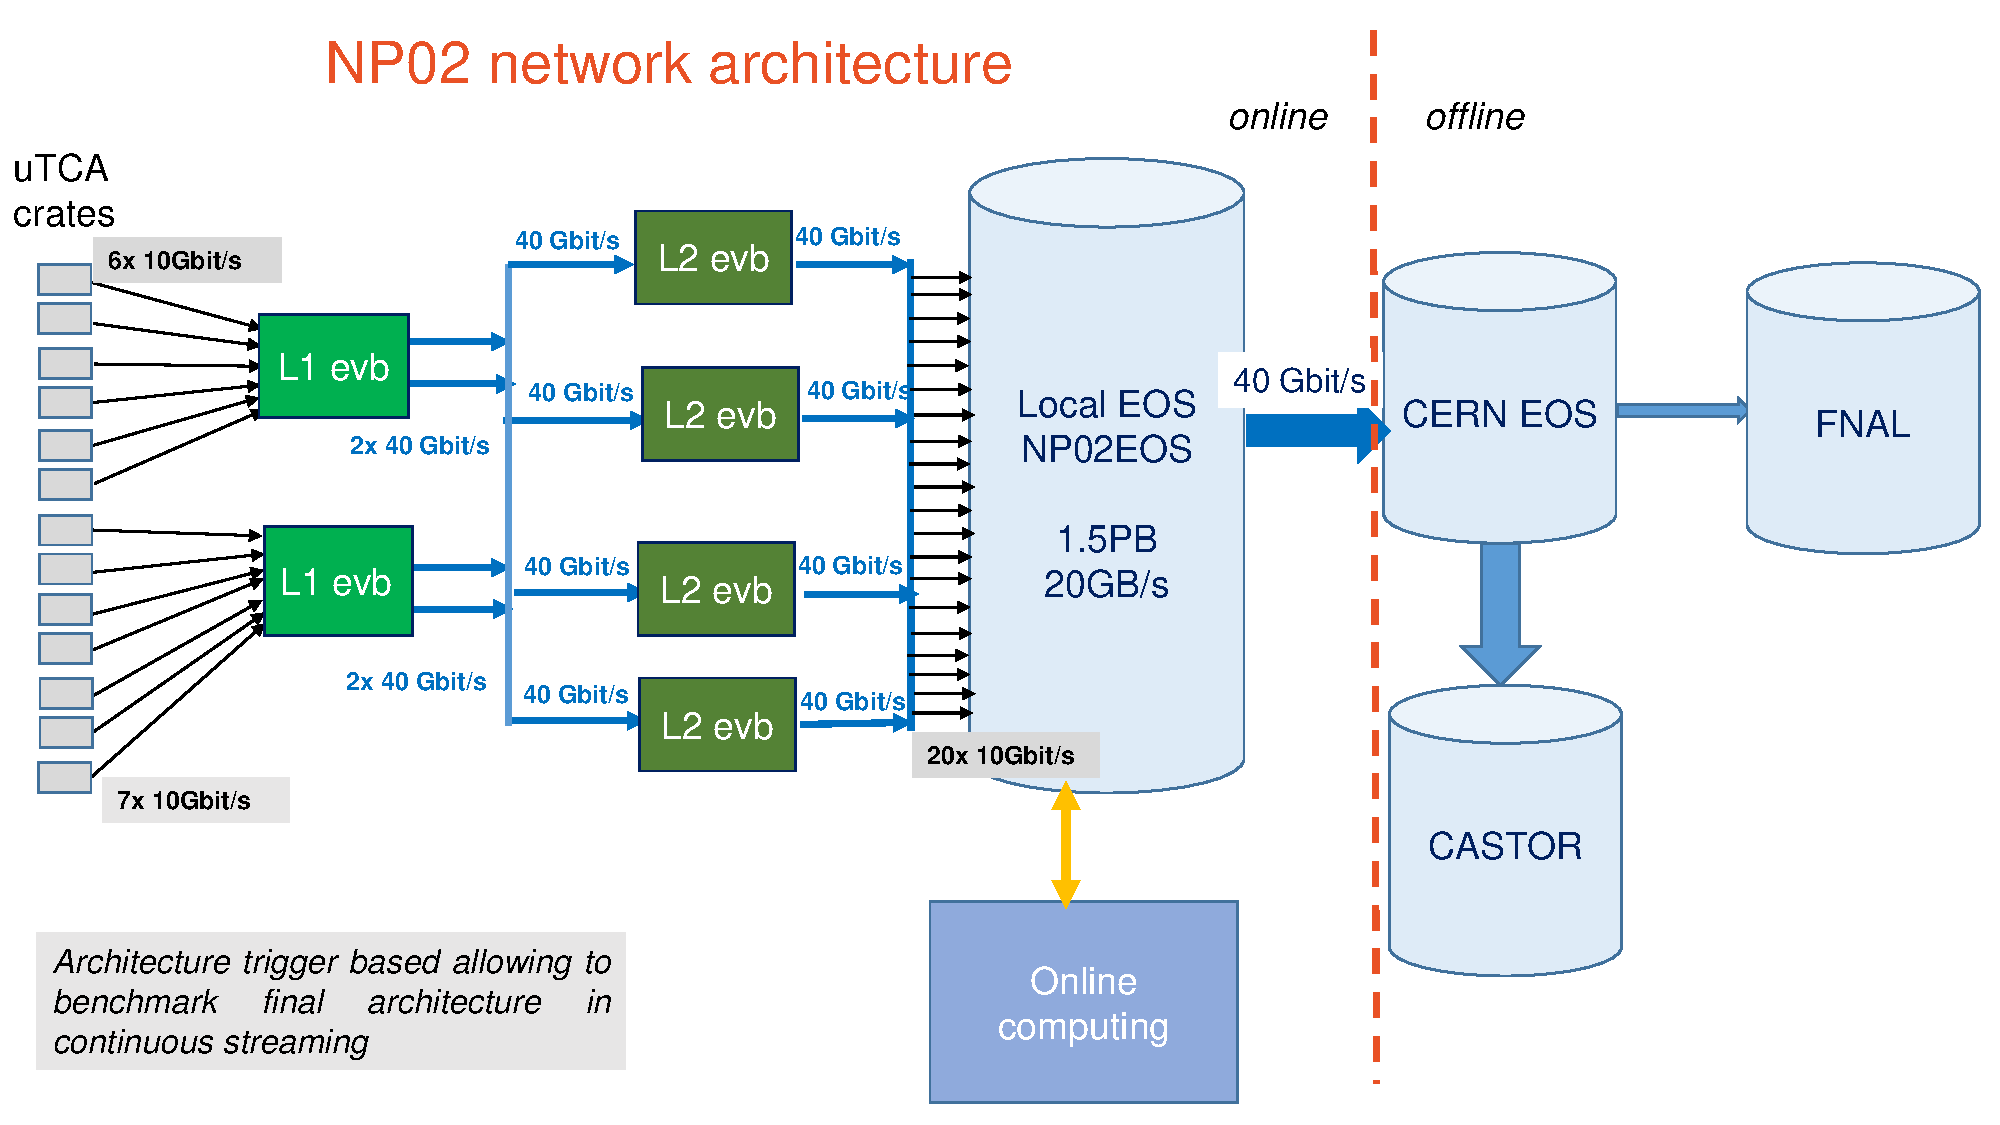
\includegraphics[width=.7\textwidth]{graphics/network.pdf} 
 \caption{ Sketch of the network architecture of the \dword{pddp} DAQ system}
 \label{fig:BE_network} 
 \end{figure}

The data acquisition in \dword{pddp} is currently trigger based. The \dword{daq} front-end transmits the data of the drift window corresponding to each trigger. The FE system consists of 12 uTCA crates for the charge readout and one crate for the light readout.  All these crates are connected to the back-end system with Ethernet optical links operating at 10 Gbit/s. A trigger server handles the white-rabbit time-stamping of external trigger signals (beam counters, cosmic counters, PMTs trigger, calibration triggers, random triggers) and the transmission of these time-stamps to the AMCs via the White-Rabbit network and of the trigger information to the L1 event builders via a dedicated Ethernet network. The White-Rabbit network ensures also the timing and synchronization of the AMC digitization units. 

Data are acquired via the the network and assembled in events in the RAM memories of the two L1 event builders {\it(np02evbl1a, np02evbl1b)}.
The task of the L1 event builder is to put together data from the uTCA crates for the same drift widow. Each event builder deals with the data corresponding to half of the detector and its architecture is based on a DELL R730 machine (384 GB RAM, 2 Intel cards R710, 2 Mellanox
Connect X3 2 ports, 40Gb/s Ethernet QSFP +, CPU type Intel XEON Gold 5122 3.6 GHz, 4 cores, 8 threads). Drift windows of events belonging to the same run are attributed the same progressive event number by the two event builders.

Data from the two L1 event builders are then sent via the network to the four L2 event builders working in parallel {\it(np02evbl2a, np02evbl2b, np02evbl2c, np02evbl2d)}. DELL R730 machines are used for this task. They have similar specifications as the L1 machines but with less network connectivity (since there is no need for the x 8 10 Gbit /s links in input). They also require less RAM memory. The configuration of these 4 machines includes: 192 GB RAM, 2 Mellanox Connect X3, CPU type Intel XEON Gold 5122 3 6 GHz, 4 cores. 

The task of the L2 event builders is to read the events halves assembled on the RAM disks of the L1 event builders and merge them to in order to  assemble the full event. The L2 event builders eventually pack together several full events in data files (run sequence data files) of 3GB size, containing up to a maximum number of triggers. These tasks are all performed on the RAM disks of the L2 machines. Each L2 event builder runs a merging process continuously selecting and copying the event halves to be included in sequence data files from the LV1 RAM disks. In order to guarantee a even sharing of the workload on the four L2 machines, the selection is performed on the basis of the progressive event number by using a fixed arithmetic events allocation rule, based on the division module: 

\begin{itemize}
 \item np02evbl2a builds event 1,5,9,13,17,...
 \item np02evbl2b builds event 2,6,10,14,18,...
 \item np02evbl2c builds event 3,7,11,15,19,...
 \item np02evbl2d builds event 4,8,12,16,20,..
 \end{itemize}

The halves of the same event available on the two L1 RAM disks are continuously merged in a single events on the L2 RAM disk. Events are then added, one after the other to the sequence data file, which is still temporary written on the L2 RAM disk.  Once the maximum number of events for a sequence file is reached, the data file is closed and its checksum value is computed. The file is immediately transferred to the online storage facility (NP02EOS), which is based on a distributed file system. The online storage facility includes and 20x24 disk units running in parallel (20  DELL R 510 machines, each one with 72 TB of available disk space, and a dedicated link of 10 Gbit/s) and operates a total disk space of 1.5 PB under the EOS distributed file system. 

In order to fully exploit the available bandwidth (20GB/s), several files may be copied in parallel simultaneously from the same event builder.  Metadata files are generated as well during the copy from the L2 RAM disk to NP02EOS. The time needed to write a single 3 GB data file is $\approx$ 4 seconds.

As soon as a sequence data file has been transferred to NP02EOS:

\begin{itemize}
\item{The file is  processed by the online processing farm: 30 servers Poweredge C6620 II, corresponding to 9270 HES06 computing units, are available. This online fast reconstruction ($\approx$ 15 seconds/event) aims at providing an online data quality monitoring}
\item {The file is copied to CERN, where it becomes available for transfer to CASTOR and FNAL}
\end{itemize}

 A MySQL database has been designed and set up in order to log the \dword{daq} activity and the  handling and processing of the online data files. In order to avoid any possible locks, each step in the files handling has its own database table: every L2 event builder  writes information about its sequence data files in a dedicated table, which is different from the table used to store information about the data transfer from the RAM disk to NP02EOS.

The overall activity of the online storage and processing farm is monitored with grafana dashboards. A run control interface ensures the control and monitoring of all the components of the system in order to start and stop runs, and check the data transfer to the local EOS. The  \dword{pddp} back-end system is shown in picture \ref{fig:BE_machines}

\begin{figure} [h!]
 \centering
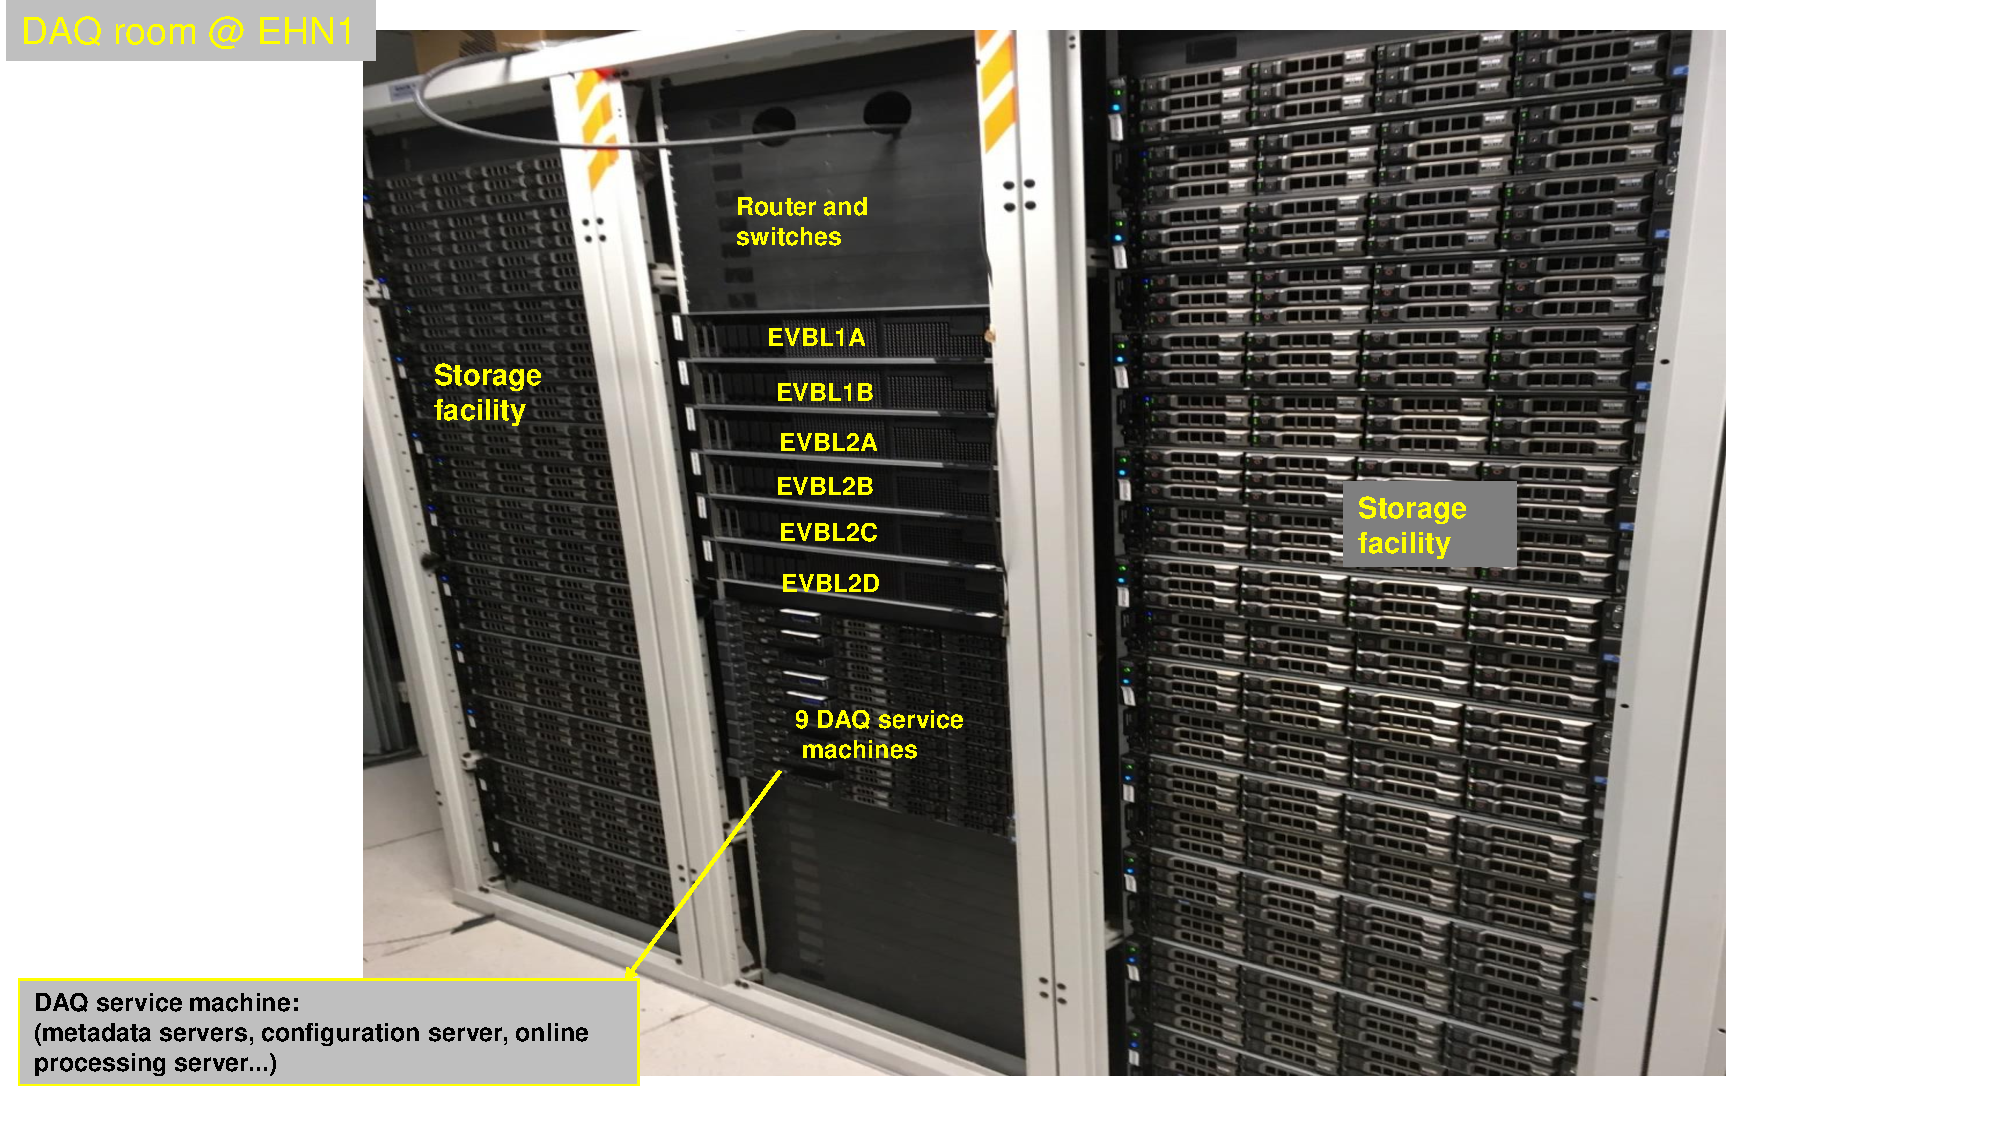
\includegraphics[width=.7\textwidth]{graphics/daqroom.pdf} 
 \caption{ Picture of the \dword{pddp} DAQ back-end system including the event builders and the online storage system, the online processing farm is not visible in this picture}
 \label{fig:BE_machines} 
 \end{figure}

The FE AMC digitization cards have also a data acquisition mode in continuous streaming with data compression which is foreseen for the trigger-less operation in \dword{dune} 10 kton. The \dword{pddp} back-end can also support this operation mode in which the trigger is defined as back-end by using the L1 event builders for memory buffering and definition of the trigger primitives, interconnected to a trigger definition node deciding which data have to be dumped on disk. The L2 machines will be then still used in order to assemble the files to be written on the distributed storage system. In this operation mode data are supposed to be decompressed on the fly by the L1 network cards in order to perform the search for the trigger primitives. A dedicated R\&D is being performed in order to optimize the decompression and trigger primitives search firmware by using Bittware FPGA cards. This firmware can be then implemented on other network cards with FPGA processing capabilities such as the \dword{felix} cards. It is foreseen in a second phase to replace the Mellanox network cards connecting the L1 event builders to the uTCA crates with \dword{felix} cards in order to have the operation mode of \dword{pddp} compatible with both the trigger based mode which has been designed for beam application and the possibility of performing full scale trigger-less tests of the \dword{dune} operation mode.

\subsubsection{\dword{pddp} Outcomes}

The installation of the \dword{daq} system of \dword{pddp} was completed in March 2019 with the installation of the digital front-end and timing systems. The \dword{daq} system was immediately operational without having to implement any configuration changes and since then it  has been constantly collecting  noise data, until August 2019 when the TPC started operating. The data taking for cosmic events started on August 29th 2019, after the Charge Readout Planes commissioning period. Since then more than 1.2 millions of cosmic events have been collected, corresponding to 130 TB. The data taking has been mostly performed with random triggers at a few 10 Hz rate given the fact that the scintillator panels in order to tag cosmic rays were not available yet. This running mode based on random triggers also allowed to stress and test the system at higher rate with respect to the one (<1 Hz) which would have been provided by the cosmic trigger panels.  Events have been also systematically been reconstructed by the online storage facility on real time.

The \dword{daq} system has shown to be very stable with no issues encountered at the level of the event builders and the associated software. The only problems occurred were related to some sporadic cooling failures of the \dword{daq} room (in common for both \dword{pdsp} and \dword{pddp}) which hosts the network infrastructure and the event builders and the storage facility. These cooling failures obliged to shut down the machines for a few hours until when the chilled water re-circulation was properly restarted by the CERN infrastructure. The back-end system implemented for \dword{pddp} is equivalent to the system which will be implemented for a dual-phase 10 kton module, it is fully interfaced with the same front-end electronics foreseen for the 10 kton module and it has shown to be working with no issues, guaranteeing a smooth detector data taking.
The online storage system of \dword{pddp} has already the capabilities to satisfy the storage needs of a \dword{dune} far detector module.


\subsection{Ongoing Development}
\label{sec:daq:design-validation}

\dword{daq} subsystem development is ongoing at \dword{protodune} at the time of
writing. A detailed schedule for 2019 is available
in \cite{bib:docdb14095}. Major development plan milestones, a number
of which have already been achieved at the time of this writing, are:
\begin{itemize}
\item optimization and tuning of the front-end readout
\item optimization and tuning of the \dword{artdaq} based dataflow software
\item enhancement of monitoring and troubleshooting capabilities
\item introduction of CPU-based hit finding (necessary for \dword{pds} readout)
\item introduction of \dword{fpga}-based hit finding (for \dword{tpc} readout)
\item implementation of online software data selection beyond trigger
primitive stage (introduction of trigger candidate generation, and
\dword{trigcommand} generation), and tests on well identified interaction
topologies (e.g. long horizontal tracks, or Michel electrons from muon decay)
\item integration of online \dword{trigcommand} and modified data flow to event
builder to facilitate self-triggering of detector
\item implementation of extended \dword{fpga}-based front-end functionality
(e.g., compression)
\item prototyping of fake \dword{snb} data flow in front end and the back end.
\end{itemize}

Below, we focus on ongoing developments related to upstream \dword{daq},
data selection, and \dword{daqccm} prototyping, which is relevant to all \dword{daq} subsystems. These are the key areas where new technologies, beyond \dword{protodune}, remain to be designed and tested.

\subsection{Plan for Future Development}
\label{sec:daq:design-plans}

As mentioned in the introduction of this section, at present, the development model chosen for the \dword{daq} system is the one of iterative prototyping.
This model is widely used in projects in which requirements are still
being refined and particularly for systems relying on rapidly evolving technologies, such as today's information and computing sector. 
This model will be used throughout 2019, making use of the \dword{protodune} setup to explore architectural options, software solutions, etc.
At a later stage, the \dword{daq} development will move to a more streamlined incremental model, ensuring that careful design precedes the final implementation of individual components.
Most of the development will be carried out emulating the data inputs.
On the other hand, the \dword{daq} will be validated regularly via test stand integration with detectors, such as \dword{protodune} or pre-installation sites.
The overall development schedule with the main \dword{daq} milestones is shown in Section~\ref{sec:daq:schedule}.

A complete demonstration system in order to test the DUNE dual-phase DAQ has been put in operation at IPNL. This system includes a charge readout uTCA crate with 10 AMC cards and a DAQ server including a FPGA network card (Bittware A10P3S with Altera Arria 10 FPGA,
4 x 40 GbE QSFP interfaces which can support  x16 10 GbE channels). The purpose of this system is to test the firmware developments in the AMCs for the DUNE continuous streaming DAQ operation and  to develop the back-end firmware for data reception, decoding, decompression and generation of trigger primitives. The data reception and real time decompression have already been implemented with a high degree of parallelism in the Arria 10 FPGA and are already operational. The implementation of the generation of the trigger primitives at the FPGA level after decompression is in progress. The digital front-end electronics at the level of the AMCs can operate in both trigger based mode (\dword{pddp}) or continuous streaming mode (\dword{dune}). This test chains allows performing all the demonstration and benchmarking steps without interfering with the ProtoDUNE-DP DAQ operation which is trigger based. This benchmarking phase is in particular useful in order to correctly dimension the DUNE DAQ for the dual-phase far detector module. The algorithms and the firmware developed on the Arria 10 FPGA could be then transported at the level of the \dword{felix} card or other DAQ elements of the DUNE DAQ. It is also foreseen to plug in the Bittware A10P3S  in \dword{pddp} by replacing or working in parallel with one of the Mellanox ethernet cards of the level 1 event builders in order to provide a direct demonstration with real data. The following step in \dword{pddp} would be to replace the Mellanox network cards which connect the L1 event builder machines to the uTCA crates with \dword{felix} cards. The FPGA in the \dword{felix} could be then used to implement the decompression and trigger primitives firmware developed in the current test bench activities.


%%%%%%


\section{Production, Assembly, Installation and Integration}
\label{sec:daq:production}

The \dword{daq} system relies largely on commercial off-the-shelf components, with the exception of the timing system and the first stage of the upstream \dword{daq}.
Therefore, the production and assembly aspects are simpler than for other systems, while of course the installation and integration stages are very important and have to be planned carefully, due to the large number of interfaces of the \dword{daq} system with other parts of the experiment.

\subsection{Production and Assembly}
\subsubsection{Timing System}


A full scale implementation of timing system for the  \dword{dune} dual-phase module has been put successfully in operation for \dword{pddp} where each \dword{utca} crate contains a \dword{wrmch} for time synchronization of the digital electronics. This timing slave unit is connected via \SI{1}{Gbit/s} optical fiber to a master node that serves as a synchronization reference for all connected slave nodes on the network. This is the same system which is foreseen for \dword{dune} where the integration with the timing for the single phase modules is foreseen by having a common high stability time source (GPS-disciplined oscillator) providing the 1PPS and 10 MHZ clock signals.

This system for \dword{pddp} time synchronization is built around the commercially available components from the \dword{wr} project\footnote{\url{https://www.ohwr.org/projects/white-rabbit}.} with custom hardware and firmware development. The system performs automatic and continuous self-calibration to account for any propagation delays and can provide sub-\si{\nano\s} accuracy for timing synchronization.

The \dword{wr} network combines the synchronous \SI{1}{Gbit/s} Ethernet (SyncE) technology with the exchange of PTPV2 packets  to synchronize clocks of distant nodes to a common time. A high-stability GPS disciplined oscillator (GPSDO) with  accuracy similar to an atomic clock provides a clock reference signal to be distributed over the physical layer interface of the \dword{wr} Ethernet network. The network topology uses specially designed switches that have standard IEEE802.1x Ethernet bridge functionality with additional \dword{wr}-specific extensions to preserve clock accuracy. Time and frequency information are distributed to the nodes on the \dword{wr} network via optical fibers. The \dword{wr} protocol automatically performs dynamic self-calibrations to account for any propagation delays and keeps all connected nodes continuously synchronized to sub-\si{\nano\second} precision. 

In the implementation specific to \dword{pddp}, a GPS-disciplined clock unit (Meinberg LANTIME M600\footnote{Meinberg\texttrademark{}, \url{https://www.meinbergglobal.com/english/products/advanced-1u-ntp-server.htm}.}) feeds \SI{10}{MHz} and \num{1}\,PPS reference signals to a commercial \dword{wr} switch (Seven Solutions WRS v3.4\footnote{Seven Solutions\texttrademark{}, \url{http://sevensols.com/index.php/products/white-rabbit-switch/}.}). The switch acts as grandmaster of the \dword{wr} network connected via \SI{1}{Gbit/s} optical links to both the dedicated \dword{wr} timestamping node (\dword{wrtsn}) and the \dword{wr} end-node slave cards present within each \dword{utca} crate (\dword{wrmch}), keeping these synchronized to its reference time. The \dword{wrgm} also communicates through a standard Ethernet port with the LANTIME unit for its date and time synchronization via \dword{ntp}. The \dword{wrtsn} module receives analog TTL-level trigger signals, generates their timestamps, and transmits them over the \dword{wr} network to the connected \dword{wrmch} units. This timestamp information is then used by \dwords{amc} to find the data frame corresponding to the trigger.  


The \dword{wrmch} card  enables clock/timing/trigger distribution to \dwords{amc}. It communicates with them via dedicated lines in the backplane of the \dword{utca} crate using a customized data-frame protocol. The module contains a commercial \dword{wr} slave node card, the \dword{wr} Lite Embedded Node (Seven Solutions OEM \dword{wr}-LEN\footnote{Seven Solutions\texttrademark{}, \url{http://sevensols.com/index.php/products/oem-wr-len/}.}), as mezzanine card. \dword{wr}-LEN runs on customized firmware that also enables it to decode the trigger timestamp data packet received over the \dword{wr} network.










\subsubsection{Upstream DAQ}
The readout part of the upstream DAQ relies on FPGA based PCIe cards (FELIX) receiving detector data. Prototype cards implementing parts of the required functionality exist already, but more prototypes are planned before the production readiness review planned in December 2022. 
While the hardware design will be done at the institutions working in this area, the production of prototypes and final cards will be outsourced, allowing for early identification of those companies that can guarantee a high quality cards production. 


\subsubsection{Racks, Servers, Storage and Network}
While commercial devices do not need to be produced or assembled, enough time has to be planned, once the proper devices are identified, for the tendering and procurement procedures. Racks and fibers will be procured in order to be available early in 2023; servers and switches will be purchased in two batches, one to be ready for supporting the installation and commissioning of the detector components and \dword{daq} infrastructure and one to reach nominal performance, in time for the start of data taking.

\subsection{Installation and Integration}


The \dword{daq} will be installed in an enclosure in the west end of the Central
Utilities Cavern (\dword{cuc}) (Figure~\ref{fig:cavern-layout}).  Roughly
half of this space will be office space (including control
workstations) and the other will be a computer room to hold the \dword{daq}
front-end computing and network equipment (Figure~\ref{fig:install-cuc}). Further details of the interface of \dword{daq} with underground facilities
may be found in \citedocdb{6988}, and the installation interface document for \dword{daq} in \citedocdb{7015}.

Infrastructure in the \dword{cuc} will be installed starting in Q4~2022
(Figure~\ref{fig:high-level-schedule}).  At that point, CF will have
handed the \dword{daq} group an empty room with cooling water and power
connections.  Over the next nine months, racks for the \dword{daq} computing
will be installed, plumbed into cooling water, and connected to power
and networking.  The network connection from this data room to the fiber
trunks going up the shaft will also be made, as will preparations to
receive the multi-mode fiber connections from the \dword{wib} to the
\dword{felix} cards housed in servers in these racks. There is space
for \cucracks racks, with 4 set aside for other consortia, 12 per
module for upstream \dword{daq} electronics, and the remaining space for
networking and other \dword{daq} computing needs. An initial engineering design of the computer room is shown in Figure~\ref{fig:daq-room}, which meets all requirements for capacity, cooling, safety and installation schedule.

\begin{dunefigure}[DAQ counting room in the CUC]{fig:daq-room}{Initial engineering design for the \dword{daq} counting room in the CUC}
 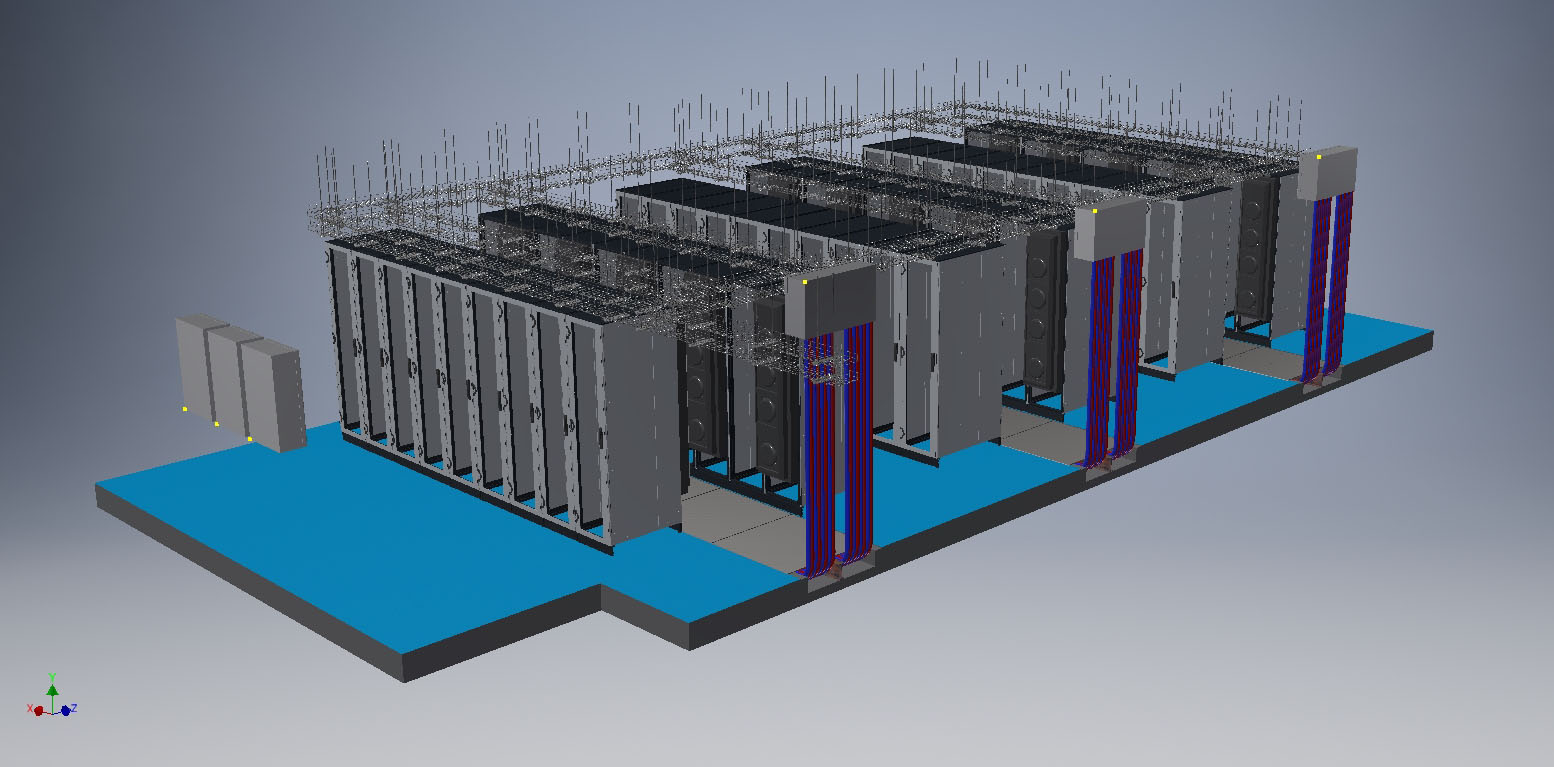
\includegraphics[width=0.9\textwidth]{daq-room.jpg}
\end{dunefigure}

Starting in Q3~2023, the data room will be ready for the installation of
the \dword{daq} servers servicing the first module described in
Section~\ref{sec:daq:considerations}.  This will proceed over the
next year, with servers being installed, cabled up, and tested.
As much configuring and commissioning work as possible will be done over
the network from the surface (or home institutions), to limit the number
of people underground.  Note that this data room is sized for all four
modules of \dword{daq} computing, so one quarter will be installed at this
point.  If more computing power is needed for the commissioning of the
first module (for example, to deal with unexpected noise levels), space
and power will be borrowed from the provision for future modules until the problems are
alleviated. 
Additional space for eight racks will be on the surface in the Ross Dry
Room. This will house the back-end computers, high level filter servers, and associated network equipment.

Starting in Q3~2025, the \dword{daq} will be ready to connect fibers to the electronics of the second detector module, to allow their commissioning.

The underground installation phase of the \dword{daq} system has the largest safety
implications, which are discussed in Section~\ref{sec:daq:safety}.

\section{Organization and Project Management}
\label{sec:daq:organization}


\subsection{Consortium Organization}

The \dword{daq} consortium was formed in 2017 as a joint single and
dual phase consortium, with a consortium leader and a technical
leader. The current organization of the consortium is shown in
Figure~\ref{fig:daq-org}. The \dword{daq} institution board currently comprises
representatives from 34 institutions as shown in Table~\ref{tab:daq-ib}. The consortium leader is the spokesperson for the consortium and responsible for the overall scientific program and management of the group. The technical leader of the consortium is responsible for
managing the project for the group. The leadership is assisted in its duties by the Project Office, populated by the Resource Manager, the Software and Firmware coordinator and the Integration and Support Coordinator, providing support in the corresponding areas. 
The consortium is organized into working groups addressing the design,
R\&D, integration, and, in the future, construction, commissioning and installation of the key \dword{daq} systems. The Physics Performance and Facility working groups are not associated to a specific system but provide oversight of the general \dword{daq} performance in the physics context and the on the interface with the facility infrastructure. The \dword{daq} working group mandates are detailed in~\citedocdb{14938}.

\begin{dunefigure}[DAQ consortium org chart]{fig:daq-org}{Organizational chart for the \dword{daq} Consortium
 }
  %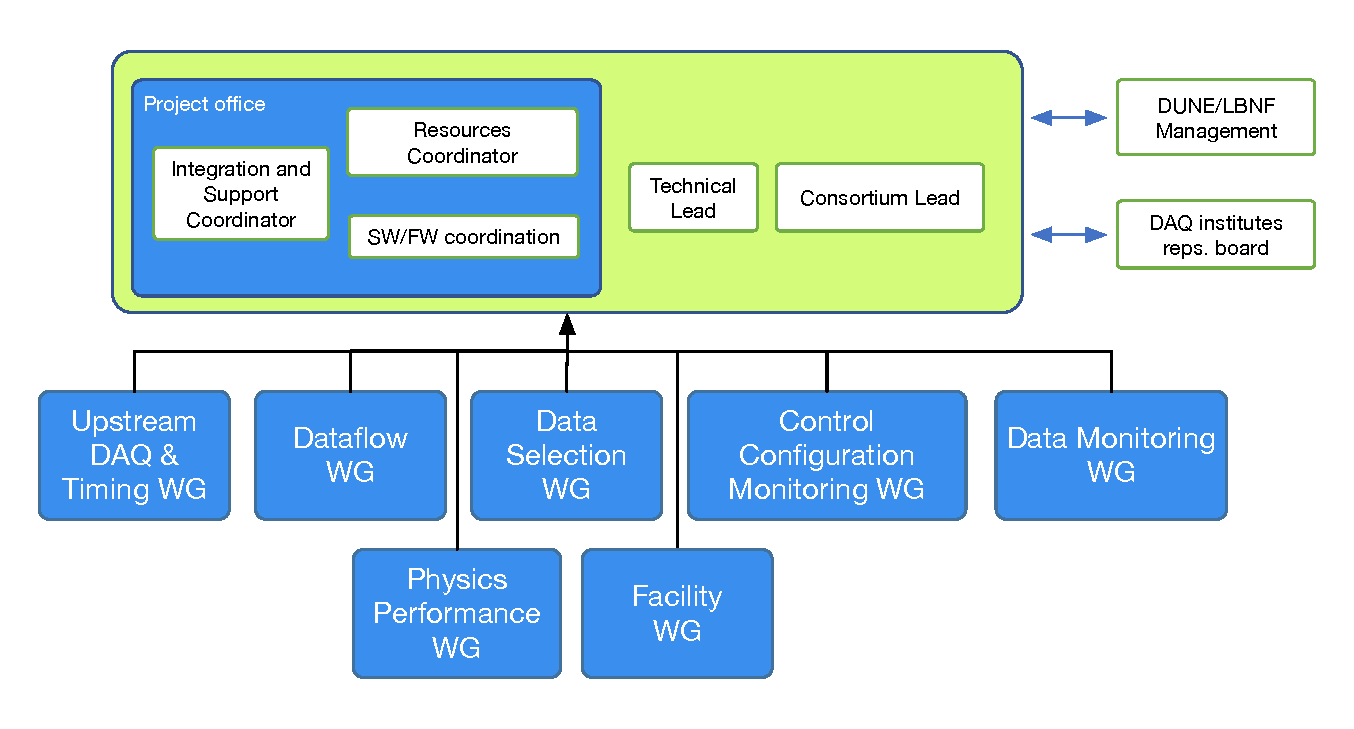
\includegraphics[width=0.9\textwidth]{daq-organogram.pdf}
\end{dunefigure}

\begin{dunetable}
[DAQ Consortium Board institutional members and countries]
{p{0.65\textwidth}p{0.25\textwidth}}
{tab:daq-ib}
{DAQ Consortium Board institutional members and countries.}   
Member Institute & Country  \\ \toprowrule
CERN & CERN     \\ \colhline
Universidad Sergio Arboleda (USA) & Colombia     \\ \colhline
Czech Technical University & Czech Republic \\ \colhline
Lyon & France \\ \colhline
INFN Bologna & Italy \\ \colhline
Iwate & Japan     \\ \colhline
KEK & Japan     \\ \colhline
NIT Kure & Japan     \\ \colhline
NIKHEF & Netherlands    \\ \colhline
University of Birmingham & UK     \\ \colhline
Bristol University & UK     \\ \colhline
University of Edinburgh & UK     \\ \colhline
Imperial College London & UK     \\ \colhline
University College London (UCL) & UK     \\ \colhline
University of Liverpool & UK     \\ \colhline
Oxford University & UK     \\ \colhline
Rutherford Appleton Lab (RAL) & UK     \\ \colhline
University of Sussex & UK     \\ \colhline
University of Warwick & UK     \\ \colhline
Brookhaven National Lab (BNL) & USA     \\ \colhline
Colorado State University (CSU) & USA     \\ \colhline
Columbia University  & USA     \\ \colhline
University of California, Davis (UCD) & USA     \\ \colhline
Duke University & USA     \\ \colhline
University of California, Irvine (UCI) & USA     \\ \colhline
Fermi National Accelerator Laboratory (Fermilab) & USA     \\ \colhline
Iowa State University & USA     \\ \colhline
University of Minnesota, Duluth (UMD) & USA     \\ \colhline
University of Notre Dame & USA     \\ \colhline
University of Pennsylvania (Penn) & USA     \\ \colhline
South Dakota School of Mines and Technology (SDSMT) & USA     \\ \colhline
Stanford Linear Accelerator Lab (SLAC) & USA     \\ \colhline
\end{dunetable}

\subsection{Schedule and Milestones}
\label{sec:daq:schedule}

The high-level \dword{daq} milestones are listed in Table~\ref{tab:daq-sched}, interleaved with the top-level DUNE project milestones, and illustrated in Figure~\ref{fig:daq:schedule}. Since the \dword{daq} project is largely based on commercial off-the-shelf components, it can be seen in the overall timeline that many of the components are procured relatively late in the project schedule.

\begin{dunetable}
[DAQ Consortium Schedule]
{p{0.65\textwidth}p{0.25\textwidth}}
{tab:daq-sched}
{\dword{daq} Consortium Schedule}   
Milestone & Date (Month YYYY)   \\ \toprowrule

Upstream \dword{daq} Architecture Technology Decision & June 2020 \\ \colhline
Engineering Design Review for Timing System &  June 2020   \\ \colhline
\rowcolor{dunepeach} Start of \dword{pdsp}-II installation& \startpduneiispinstall      \\ \colhline
Production Readiness Review for Timing System & June 2021 \\ \colhline
Preliminary Software Design Review & January 2022 \\ \colhline
Engineering Design Review for Hardware/Firmware & March 2022 \\  \colhline
\rowcolor{dunepeach} Start of \dword{pddp}-II installation& \startpduneiidpinstall      \\ \colhline
 \dword{prr} dates &      \\ \colhline
Start of  (component 1) production  &      \\ \colhline
Start of (component 2) production  &      \\ \colhline
Start of  (component 3) production  &      \\ \colhline
\rowcolor{dunepeach}South Dakota Logistics Warehouse available& \sdlwavailable      \\ \colhline
Start of Racks Procurement & July 2022  \\ \colhline
Start of \dword{daq} Server Procurement (I) & September 2022  \\ \colhline
\rowcolor{dunepeach}Beneficial occupancy of cavern 1 and \dword{cuc}& \cucbenocc      \\ \colhline
Production Readiness Review for Readout Hardware/Firmware & December 2022  \\ \colhline
End of Racks Procurement & March 2023  \\ \colhline
Start of  \dword{daq} Custom Hardware Production &  March 2023    \\ \colhline
\rowcolor{dunepeach} \dword{cuc} counting room accessible& \accesscuccountrm      \\ \colhline
End of \dword{daq} Server Procurement (I) & May 2023  \\ \colhline
Start of \dword{daq} Installation & May 2023 \\ \colhline
\dword{daq} Software Final Design Review & June 2023  \\ \colhline

End of  \dword{daq} Custom Hardware Production &  December 2023    \\ \colhline
\rowcolor{dunepeach}Top of \dword{detmodule} \#1 cryostat accessible& \accesstopfirstcryo      \\ \colhline
End of  (component 1) production  &      \\ \colhline
... & ...                       \\ \colhline
\rowcolor{dunepeach}Start of \dword{detmodule} \#1 TPC installation& \startfirsttpcinstall      \\ \colhline
Start of \dword{daq} Server Procurement  (II) & September 2024  \\ \colhline
\rowcolor{dunepeach}Top of \dword{detmodule} \#2 accessible& \accesstopsecondcryo      \\ \colhline

End of \dword{daq} Server Procurement  (II) & May 2025  \\ \colhline
End of \dword{daq} installation & May 2025 \\ \colhline
\rowcolor{dunepeach}End of \dword{detmodule} \#1 TPC installation& \firsttpcinstallend      \\ \colhline
\rowcolor{dunepeach}Top of \dword{detmodule} \#2 accessible& \accesstopsecondcryo      \\ \colhline
 \rowcolor{dunepeach}Start of \dword{detmodule} \#2 TPC installation& \startsecondtpcinstall      \\ \colhline
End of \dword{daq} Standalone Commissioning & December 2025 \\ \colhline
\rowcolor{dunepeach}End of \dword{detmodule} \#2 TPC installation& \secondtpcinstallend      \\ \colhline
\dword{daq} Server Procurement  (III) & July 2026  \\ \colhline
End of \dword{daq} Commissioning & December 2026  \\ 
\end{dunetable}

\begin{dunefigure}[DAQ schedule for first \SI{10}{\kilo\tonne} module]{fig:daq-schedule}{\dword{daq} schedule for first \SI{10}{\kilo\tonne} module. \label{fig:daq:schedule}}
  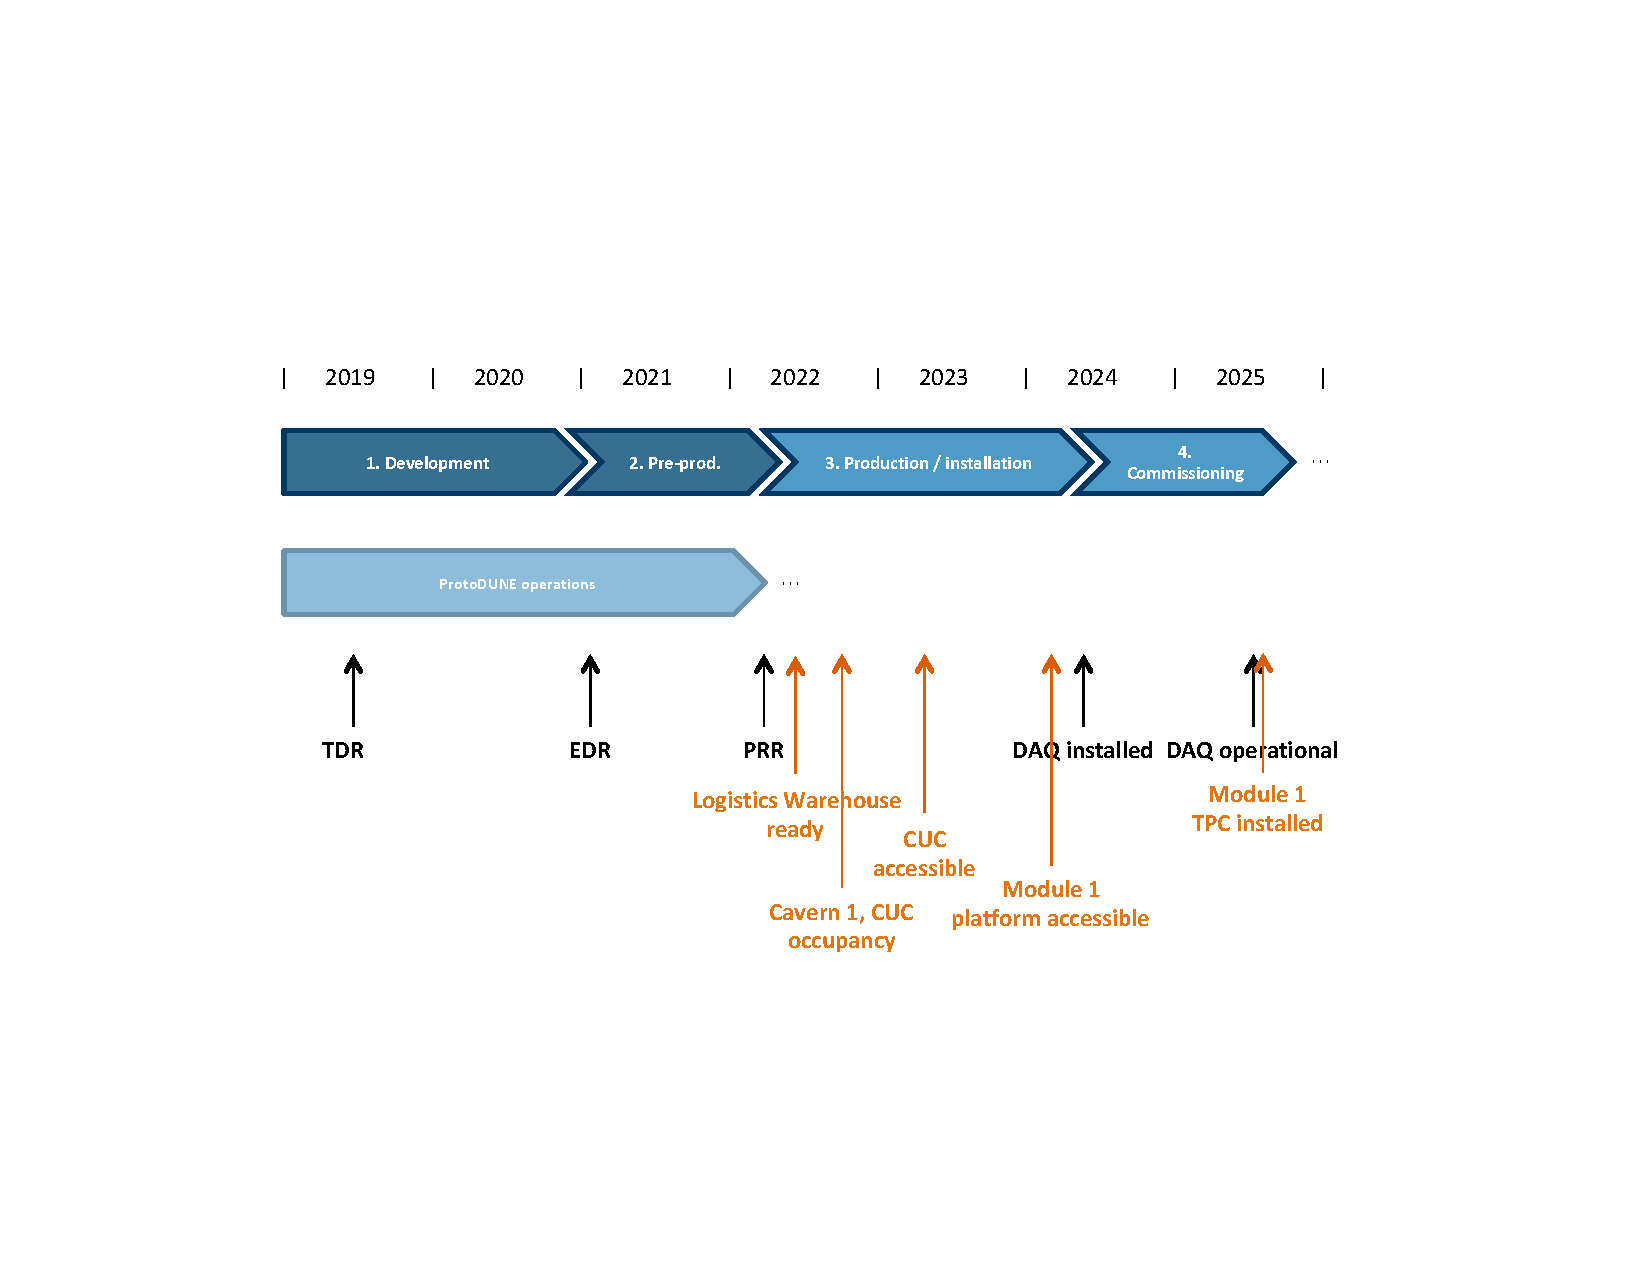
\includegraphics[width=0.95\textwidth,clip,trim=1cm 2cm 1cm 2cm]{daq-schedule.pdf}
\end{dunefigure}


\subsection{Safety and Risks}
\label{sec:daq:safety}

Personnel safety during design, construction, testing, installation, and
commissioning of the system is crucial for the success of the
project. Detector safety during installation,
commissioning and operations is also key to project success.
The consortium will strictly follow ES\&H guidelines for the
project as well as follow the safety rules of the institutions where
the work is performed, including national laboratories, SURF, and
participating universities.  

Two overall safety plans will be followed by the FD \dword{daq}. General work underground will comply
with all safety procedures in place for working in the detector
caverns and in the \dword{cuc} underground at
SURF. \dword{daq}-specific procedures for working with racks full of
electronics or computers, as defined 
at Fermilab, will be followed, especially with respect to electrical safety and the fire suppression
system chosen for the counting room. For example, a glass wall between the server room space and
the other areas in the CUC will be necessary to prevent workers in the server room from being
unseen if they are in distress, and an adequate hearing protection
regime must be put in place.

There are no other special safety items for the \dword{daq} system not already covered by the more general safety plans. The long-term emphasis is on remote operations capability from around the world, limiting the need for physical presence at SURF, and with underground access required only for urgent interventions or hardware replacement. 

A set of risks to the successful construction and operation of the \dword{daq} system has been
identified by the consortium, and is provided,
together with mitigation strategies and pre-mitigation risk level, 
in Table~\ref{tab:risks:SP-FD-DAQ}. Post-mitigation risk levels are
currently being re-evaluated. Risk is quantified with respect to
probability, cost impact, and schedule impact. High (H), medium (M), and low (L)
probability is identified as
$>25$\%, $10-25$\%, and $<10$\%, respectively; high (H), medium (M), and low (L)
cost impact is identified as
$>20$\%, $5-20$\%, and $<5$\% cost increase, respectively; and high
(H), medium (M), and low (L) schedule impact is identified as 
$>6$ months, $2-6$ months, and $<2$ months delay, respectively.


% risk table values for subsystem SP-FD-DAQ
\begin{longtable}{p{0.18\textwidth}p{0.20\textwidth}p{0.32\textwidth}p{0.02\textwidth}p{0.02\textwidth}p{0.02\textwidth}} 
\caption{Risks for SP-FD-DAQ \fixmehl{ref \texttt{tab:risks:SP-FD-DAQ}}} \\
\rowcolor{dunesky}
ID & Risk & Mitigation & P & C & S  \\  \colhline
RT-SP-DAQ-01 & Detector noise specs not met & ProtoDUNE experience with noise levels and provisions for data processing redundancy in DAQ system (upstream DAQ FPGA/CPU and high level filter) & H & M & H  \\  \colhline
RT-SP-DAQ-02 & Externally-driven schedule change & Provisions for standalone testing and commissioning of production DAQ components, and schedule adjustment & H &  & M \\  \colhline
RT-SP-DAQ-03 & Lack of expert personnel & Resource-loaded plan for DAQ backed by institutional commitments, and schedule adjustment using float & H &  &  \\  \colhline
RT-SP-DAQ-04 & Power/space requirements exceed CUC capacity & Sufficient bandwidth to surface and move module 3/4 components to an expanded surface facility & H & M & H \\  \colhline
RT-SP-DAQ-05 & Excess fake trigger rate from instrumental effects & ProtoDUNE performance experience, and provisions for increase in event builder, high level filter, and upstream DAQ processing capacity, as needed & M & M & H  \\  \colhline
RT-SP-DAQ-06 & Calibration requirements exceed acceptable data rate & Provisions for increase in event builder and high level filter capacity, as neeed & M & L & M \\  \colhline
RT-SP-DAQ-07 & Cost/performance of hardware/computing excessive & Have prototyping and pre-production phases, reduce performance using margin or identify additional funds & M &  &  \\  \colhline
RT-SP-DAQ-08 & Optical components obsolete before production & Market survey, commercial standards, and design changes & H  &  &  \\  \colhline
RT-SP-DAQ-09 & Insufficient FPGA processing resources & ProtoDUNE and simulation experience, FPGA replacement, or sustain increased data rates & H  & H  & H  \\  \colhline
RT-SP-DAQ-10 & Insufficient throughput in computing system & Design allows for expansion; expand system capacity for throughput before commissioning & H  & M & H  \\  \colhline
RT-SP-DAQ-11 & Event builder throughput insufficient & Design allows for expansion; expand system capacity for throughput before commissioning & H  & M & M \\  \colhline
RT-SP-DAQ-12 & Additional data reduction steps required after event building & Provisions for increase in high level filter capacity, as needed & H  & L & M \\  \colhline
RT-SP-DAQ-13 & PDTS fails to scale for DUNE requirements & Hardware upgrade & M & L & H  \\  \colhline
RT-SP-DAQ-14 & Full remote operation of DAQ proves non-viable & Pre-production operation testing and allocation of surface or underground space for on-site operations & M &  & M \\  \colhline
RT-SP-DAQ-15 & DAQ system does not meet overall DUNE uptime specification & Extensive QA and exercise of failure mode recovery in extended ProtoDUNE runs, and replacement of components & H  &  & M \\  \colhline
RT-SP-DAQ-16 & External services do not allow reliable operation of DAQ system & Performance specifications for external services, prior to construction. & H  & L & H  \\  \colhline

\label{tab:risks:SP-FD-DAQ}
\end{longtable}
%\fixme{anne to uncomment}

The following risks and mitigation strategies have been identified:

\begin{description}
\item[Detector noise specs not met] Excessive noise will make it
  impossible for the \dword{daqdss} to meet physics goals while
  generating reasonable data volumes. Prior (to construction) mitigation includes
  studying noise conditions at \dword{protodune}, and leaving provisions in the
  system for additional front-end filtering (in the form of the
  upstream \dword{daq} upgradable processing resources) and/or post-event builder processing (in
  the form of the high level filter). Mitigation (post-construction) includes augmenting
  filtering resources using a larger computing system for the high
  level filter.

\item[Externally-driven schedule change] The \dword{daq} has schedule links during
  testing, construction, and installation phases with most other
  subsystems. Schedule slip elsewhere will potentially cause
  delay to the \dword{daq}. Prior mitigation includes making provisions for
  stand-alone testing and commissioning of \dword{daq} components, in the form
  of vertical and horizontal slice tests, at \dword{protodune} or
  elsewhere. Mitigation includes adjusting schedule for stand-alone
  testing and commissioning phases. 

\item[Lack of expert personnel] A significant number of experts in
  hardware, software, firmware are needed, and must be sustained
  throughout the project. Lack of personnel will increase technical
  risks and cause delay. Prior mitigation includes developing a full
  resource-loaded plan for \dword{daq}, backed by national and institutional
  commitments, and avoiding single points of failure. Mitigation
  includes adaptation of the \dword{daq} schedule, using schedule float.

\item[Power/space requirements exceed CUC capacity] The CUC has fixed
  space and power allocation for \dword{daq} 
that cannot be exceeded.  Prior mitigation includes allowing
sufficient bandwidth up the shafts to move the upstream \dword{daq} components for
subsequent DUNE far detector modules (modules 3 and 4) to the
surface, or moving some of the \dword{daq} components to the detector caverns,
and carrying out a feasibility study for doing so. 
Mitigation includes expending additional resources on an
expanded surface facility.

\item[Excess fake trigger rate from instrumental effects] Instrumental
  effects (beyond excessive noise) can cause fake triggers. Prior
  mitigation includes studying \dword{protodune} performance in detail, and monitoring detector
  performance during installation. Mitigation includes substantially increasing
  data volume, and increasing processing resources in the high level
  filter.

\item[Calibration requirements exceed acceptable data rate]
  Calibration schemes may require substantial data 
volumes, far in excess of triggered data volume, beyond currently
envisioned; e.g., due to offline analysis inefficiencies. Prior
mitigation includes allowing for back-end (\dword{eb}) system expansion to cope
with the increased data rate, and allowing for a high-level filter data
selections stage to carry out online analysis and data
reduction. Mitigation includes increasing the back-end \dword{daq} and high
level filter system capacity. 

\item[Cost/performance of hardware/computing excessive] Costs of
  system-as-designed may exceed available budget, due to the IT technology (FPGA, servers, storage) market evolving in an unfavorable way. Prior mitigation
  includes the planning of prototyping and pre-construction phases to allow
  realistic appraisal of system costs, and applying sufficient margin
  in performance estimates.  Mitigation includes reducing performance
  or identifying additional funds. 


\item[\dword{protodune} timing system fails to scale for DUNE requirements] The \dword{protodune} timing system concept may
  not scale to DUNE in scale or performance.  Prior mitigation
  includes testing the system at realistic scale before the final
  design. Mitigation includes replacing the system with upgraded
  hardware.

\item[WAN network] The network connectivity to the experiment from
  remote locations may be proven unstable, making remote control and monitoring
  inefficient. Prior mitigation includes ensuring that minimal human intervention
  is needed on the system for steady data taking and that automated
  error recovery is well developed. Mitigation includes effort to further
  improve automated data taking, and increased cost for improving network
  connectivity. In the worst case, one would foresee presence of personnel at SURF.

\item[Infrastructure] The power/cooling systems on which the \dword{daq}
  relies on cause more frequent than expected downtime. Prior
  mitigation includes designing, wherever possible, independent and redundant
  systems. Mitigation includes adding more uninterruptible power
  supplies, and improving the water cooling system to overcome otherwise
  degraded experiment uptime. 

\item[Custom electronics manufacturing issues] Large-scale production of high-speed custom
  electronics proves challenging, resulting in \dword{daq} installation delays. Prior mitigation includes diversifying manufacturers used for prototype production; assess manufacturer capability to meet specifications.  Mitigation includes running early pre-production with selected manufacturers, applying stringent QA criteria to ensure compliance with specifications.

\end{description}
